\documentclass[11pt]{article}
\usepackage[margin=1in]{geometry}
\usepackage{amsmath,amssymb,amsthm}
\usepackage{listings}
\usepackage{xcolor}
\usepackage{tikz}
\usepackage{booktabs}
\usepackage{array}
\usepackage{hyperref}
\hypersetup{colorlinks=true, linkcolor=blue!50!black, urlcolor=blue!50!black}
\usetikzlibrary{positioning,arrows.meta,fit,backgrounds}
\usetikzlibrary{calc}
\theoremstyle{definition}
\newtheorem{definition}{Definition}
\newtheorem{proposition}{Proposition}
\newtheorem{lemma}{Lemma}
\newtheorem{theorem}{Theorem}
\newtheorem{example}{Example}

\newtheorem{remark}{remark}

\newtheorem{corollary}{corollary}
\lstset{basicstyle=\ttfamily\small, breaklines=true,
        commentstyle=\color{gray}, showstringspaces=false}
\lstset{
  basicstyle=\ttfamily\small,
  keywordstyle=\color{blue!60!black}\bfseries,
  commentstyle=\color{green!40!black}\itshape,
  stringstyle=\color{orange!70!black},
  showstringspaces=false,
  breaklines=true,
  frame=single,
  rulecolor=\color{black!25},
  language=Python,
}
\title{A Recursive Notation over $\{1,2,3\}$ for Integers Coprime to Six,\\
       with an Application to Difference-of-Squares Factorisation}
\author{Shaimaa Soltan}
\date{\today}

\begin{document}
\maketitle

\begin{abstract}
We define a canonical notation writing every positive integer using only the
atoms $1,2,3$, multiplication, and the operations $\pm 1$. The construction
rests on the observation that every integer coprime to $6$ has the form
$2\cdot 3\cdot k \pm 1$ for a unique $k$ and a forced sign. Applying the rule
recursively to $k$ terminates, since each level divides the argument by
approximately six. We prove that the representation is unique once prime
factorisation is applied first, and that it is self-verifying: the expression
evaluates to the number it denotes. We then record a companion identity for
differences of squares and the enumeration of Pythagorean partners it yields.
\end{abstract}

\section{The $6k\pm1$ notation}

\begin{definition}[Atoms and forms]
An \emph{expression} is built from the atoms $1,2,3$ by multiplication and by
the two unary operations $x \mapsto 2\cdot 3\cdot x - 1$ and
$x \mapsto 2\cdot 3\cdot x + 1$.
\end{definition}

\begin{proposition}[Trichotomy modulo six]
Let $n$ be a positive integer with $\gcd(n,6)=1$. Then exactly one of
\[
  n = 6k-1, \qquad n = 6k+1
\]
holds, with $k$ a uniquely determined positive integer.
\end{proposition}

\begin{proof}
The residues coprime to $6$ are $1$ and $5$. If $n \equiv 1$, then
$k=(n-1)/6$; if $n \equiv 5$, then $k=(n+1)/6$. In each case $k$ is an integer
and the other equation has no integral solution.
\end{proof}

\begin{proposition}[Closure and sign parity]
The set $\{n : \gcd(n,6)=1\}$ is closed under multiplication, and
\[
  (6a-1)(6b-1) \equiv +1, \quad
  (6a-1)(6b+1) \equiv -1, \quad
  (6a+1)(6b+1) \equiv +1 \pmod 6 .
\]
Consequently $(6k-1)^r \equiv (-1)^r$ and $(6k+1)^r \equiv +1 \pmod 6$ for all
$r>0$.
\end{proposition}

\begin{theorem}[Existence, uniqueness, termination]\label{thm:canonical}
Every positive integer $n$ admits exactly one expression obtained by the rule
\begin{enumerate}
  \item factor $n$ into primes and write the expression as the product of the
        expressions of its prime factors;
  \item for a prime $p \le 3$, the expression is the atom itself;
  \item for a prime $p>3$, write $p = 6k \pm 1$ with the sign forced by
        $p \bmod 6$, and recurse on $k$.
\end{enumerate}
The recursion terminates.
\end{theorem}

\begin{proof}
Uniqueness of step 1 is the fundamental theorem of arithmetic; uniqueness of
step 3 is the previous proposition. For termination, note $k < p/5$ for
$p>3$, so the argument strictly decreases at each level and the descent
reaches an atom in $O(\log n)$ steps.
\end{proof}

\begin{example}
\[
\begin{aligned}
 41 &= (2\cdot3\cdot(2\cdot3+1)-1), &
 25 &= (2\cdot3-1)\cdot(2\cdot3-1), \\
 35 &= (2\cdot3-1)\cdot(2\cdot3+1), &
 97 &= (2\cdot3\cdot(2\cdot2\cdot2\cdot2)+1).
\end{aligned}
\]
\end{example}

\begin{proposition}[Structural reading]
In the canonical expression of $n$, the outermost operation is a product if
and only if $n$ is composite, and is $\pm1$ if and only if $n$ is prime.
\end{proposition}

\begin{remark}
The notation is a $\emph{certificate}$, not a test. Verifying a given expression
costs $O(\log n)$ arithmetic operations, whereas producing it requires the
prime factorisation of $n$. The $\pm1$ layer carries no multiplicative
information: for any $n = 6k\pm1$ one has $n \equiv \pm 1 \pmod k$, so no level
of the descent shares a factor with the level below it.
\end{remark}

\begin{proposition}[Perfect-power splittings]
If $n+1 = s^m$ then $(s-1) \mid n$, and if $n-1 = s^m$ with $m$ odd then
$(s+1) \mid n$, by
\[
  s^m - 1 = (s-1)\sum_{j=0}^{m-1} s^{j}, \qquad
  s^m + 1 = (s+1)\sum_{j=0}^{m-1} (-1)^{j} s^{j}.
\]
\end{proposition}

\begin{example}
$215 = 6^3-1 = 5\cdot 43$ and $217 = 6^3+1 = 7\cdot 31$.
\end{example}

\section{The difference-of-squares identity}

\begin{proposition}[Gap identity]
For $B = A + d$,
\[
  B^2 - A^2 = 2Ad + d^2 = d\,(2A+d).
\]
\end{proposition}

\begin{corollary}
For odd $n$, every factorisation $n = d\,(2A+d)$ corresponds to a divisor
$d \mid n$ with $A = (n-d^2)/(2d)$, and conversely. In particular $d=1$ always
yields the trivial factorisation $n = 1 \cdot n$.
\end{corollary}

\begin{proposition}[Two parametrisations]
The equation $n = ab$ may be solved by fixing either unknown:
\[
  \text{fix } d \text{ and solve for } A
  \;\;\Longrightarrow\;\; \text{trial division},
  \qquad
  \text{fix } x \text{ and solve for } y \text{ in } n = x^2-y^2
  \;\;\Longrightarrow\;\; \text{Fermat's method}.
\]
The first is efficient when $n$ has a small factor, the second when the factors
are close together; the cost of Fermat's method is $\approx y^2/(2\sqrt{n})$
steps.
\end{proposition}

\begin{proposition}[Wheel restriction]
If $\gcd(n,6)=1$ then every divisor of $n$ is of the form $6k\pm1$. Hence a
trial-division search need only test candidates in these two residue classes,
eliminating four of every six.
\end{proposition}

\section{Pythagorean partners}\label{sec:partners}

\begin{definition}
For a positive integer $A$, a \emph{partner} of $A$ is a pair $(B,C)$ of
positive integers with $B^2 - A^2 = C^2$.
\end{definition}

\begin{theorem}[Enumeration of partners]
The partners of $A$ are in bijection with the factorisations $A^2 = de$ with
$d<e$ and $d \equiv e \pmod 2$, via
\[
  B = \frac{d+e}{2}, \qquad C = \frac{e-d}{2}.
\]
\end{theorem}

\begin{proof}
$B^2-C^2 = (B-C)(B+C) = de = A^2$. Conversely, given $B>C>0$ with
$B^2-C^2=A^2$, set $d=B-C$ and $e=B+C$; then $de=A^2$ and $d\equiv e \pmod 2$
since $B,C$ are integers.
\end{proof}

\begin{corollary}
The number of partners of $A$ is determined by the divisor count of $A^2$. In
particular $A$ prime admits exactly one partner, namely
$\bigl((A^2+1)/2,\ (A^2-1)/2\bigr)$.
\end{corollary}

\begin{proposition}[Sum--difference conversion]
The identity
\[
  p^2 + q^2 = n^2 \iff (p-q)^2 + (p+q)^2 = 2n^2
\]
converts Pythagorean triples with hypotenuse $n$ into representations of
$2n^2$ as a sum of two squares.
\end{proposition}

\section{Implementation}

\begin{lstlisting}[language=Python]
from math import isqrt

def smallest_factor(n):
    for d in (2, 3):
        if n % d == 0:
            return d
    k = 1
    while True:
        for d in (6*k - 1, 6*k + 1):
            if d * d > n:
                return n
            if n % d == 0:
                return d
        k += 1

def rep(n):
    if n <= 3:
        return str(n)
    p = smallest_factor(n)
    if p != n:
        return rep(p) + "*" + rep(n // p)
    k = (n + 1) // 6 if (n + 1) % 6 == 0 else (n - 1) // 6
    s = "-" if (n + 1) % 6 == 0 else "+"
    core = "2*3" if k == 1 else "2*3*" + rep(k)
    return "(" + core + s + "1)"

def partners(A):
    out, n = [], A * A
    for d in range(1, isqrt(n) + 1):
        if n % d == 0:
            e = n // d
            if d < e and (d + e) % 2 == 0:
                out.append(((d + e) // 2, (e - d) // 2))
    return out
\end{lstlisting}

\begin{proposition}[Verification]
For all $n$ with $\gcd(n,6)=1$ and $n < 10^{5}$, the expression produced by
\texttt{rep} evaluates to $n$, and no two distinct $n$ produce the same
expression. Expression lengths in this range have maximum $55$ characters
(attained at $n = 96875 = 5^5\cdot 31$) and mean $40.3$.
\end{proposition}

\section{Positional interpretation: base six with a signed unit digit}

\begin{proposition}[Digit reading]
Let $\gcd(n,6)=1$ and let $n = 6k+\varepsilon$ with $\varepsilon\in\{-1,+1\}$
forced by $n \bmod 6$. Then the descent
\[
  n \;\longmapsto\; k \;\longmapsto\; \dots
\]
is a positional expansion in base six in which the unit digit is written
$\pm 1$ rather than as a residue in $\{1,5\}$, and in which the leading part is
re-expanded by the same rule.
\end{proposition}

\begin{example}
$41 = 105_6$, and $105_6 = 6\cdot 7 - 1$ with $7 = 11_6 = 6\cdot 1 + 1$, giving
$(2\cdot3\cdot(2\cdot3+1)-1)$.
\end{example}

\begin{corollary}[Depth bound]
The descent applied to $n$ terminates after at most
$\lceil \log_6 n \rceil$ levels.
\end{corollary}

\section{Minimality of the canonical form}

\begin{definition}
The \emph{size} of an expression is its number of atoms plus its number of
operations.
\end{definition}

\begin{theorem}[Shortest descent]
Among all expressions for a prime $p>3$ built from the atoms $\{1,2,3\}$ by
multiplication and $\pm1$, the canonical form obtained by the rule
$p = 6k\pm 1$ has minimal depth.
\end{theorem}

\begin{proof}
Any expression for $p$ ending in $\pm1$ has the form $mq \pm 1$ with $m$ a
product of atoms; since $p \equiv \pm1 \pmod 6$ and $2,3 \nmid p$, the largest
admissible $m$ is $6$. Every level therefore reduces the argument by a factor
of at most six, and the canonical rule attains this bound at every level.
Induction on $n$ gives the claim.
\end{proof}

\begin{remark}
The count of expressions of a given size may be obtained by dynamic
programming over the grammar
$E \to 2 \mid 3 \mid E\times E \mid E+1 \mid E-1$,
tabulating for each size the multiset of representable values. Without a size
bound the count is infinite, since $n \mapsto (n+1)-1$ pads any expression.
\end{remark}

\section{The coprimality lemma}

\begin{lemma}[Levels are coprime]\label{lem:coprime}
Let $n = 6k \pm 1$. Then
\[
  n \equiv \pm 1 \pmod{k}, \qquad\text{hence}\qquad \gcd(n,k)=1 .
\]
\end{lemma}

\begin{proof}
Immediate from $n \mp 1 = 6k$.
\end{proof}

\begin{corollary}[Negative results]\label{cor:negative}
Lemma~\ref{lem:coprime} excludes the following as factorisation aids:
\begin{enumerate}
  \item \emph{Inner divisors.} No value appearing at a level of the descent
        below $n$ divides $n$ by construction; the level immediately below
        leaves remainder $\pm 1$ exactly.
  \item \emph{Neighbour tests.} Since $n = 6(k\mp1) \pm 7$ and
        $n = 6(k\pm1) \mp 5$, one has $n \bmod (k\pm1) \in \{5,7,-5,-7\}$, so
        $k\pm1$ divides $n$ only when $k\pm1 \in \{5,7\}$, i.e.\ only for
        $n \in \{25,35,49\}$.
  \item \emph{Sign counting.} The descent of $n$ has at most
        $\lceil\log_6 n\rceil$ levels, so any statistic computed from the
        multiset of signs takes $O(\log^2 n)$ distinct values, whereas
        $\pi(n) \sim n/\log n$. By the pigeonhole principle no such statistic
        separates primes from composites.
\end{enumerate}
\end{corollary}

\begin{example}
$11$ and $35$ both have canonical forms with one $-1$ and no $+1$; $37$ and
$25$ both have one $+1$ and no $-1$. In each pair one entry is prime and the
other is not.
\end{example}

\section{Expression statistics}

\begin{proposition}[Measured lengths]
Over all $n$ with $\gcd(n,6)=1$ and $n < 10^{5}$ (a set of $33{,}333$
integers), the canonical expression produced by \texttt{rep} satisfies:
\begin{center}
\begin{tabular}{ll}
  maximum length & $55$ characters, attained at $n = 96875 = 5^5\cdot 31$ \\
  mean length    & $40.3$ characters \\
  evaluation     & $\mathrm{eval}(\mathrm{rep}(n)) = n$ for every such $n$ \\
  collisions     & none: $\mathrm{rep}$ is injective on this range
\end{tabular}
\end{center}
\end{proposition}

\begin{remark}
Length is driven by two independent quantities: the number of prime factors,
whose expressions are concatenated, and the depth of each factor's descent,
which is $O(\log p)$. The observed growth is consistent with
$O(\Omega(n)\log n)$, where $\Omega$ counts prime factors with multiplicity.
The extremal case $5^5\cdot 31$ is extremal for the first reason rather than
the second.
\end{remark}

\section{Limits of the notation}

\begin{proposition}[Primality is visible but not computable from the form]
Let $n>3$ with $\gcd(n,6)=1$. In the canonical expression of $n$, the
outermost operation is a product if and only if $n$ is composite. However,
producing that expression requires the prime factorisation of $n$, and
verifying a given expression costs $O(\log n)$ operations.
\end{proposition}

\begin{remark}[Certificate, not test]
The notation is therefore a \emph{certificate format}. It records the complete
multiplicative structure of $n$ in a string over $\{1,2,3\}$ that is
self-verifying: no external table, no oracle, and no trust in the producer are
required to check it. This is a strictly weaker property than decidability of
the structure, and the distinction is not repaired by any re-encoding, since
by Corollary~\ref{cor:negative} the additive $\pm1$ layer and the
multiplicative layer share no information.
\end{remark}

\begin{remark}[Comparison with primality testing]
Primality itself lies in $\mathrm{P}$, and in practice Miller--Rabin decides it
in $O(\log^3 n)$ time without producing any factorisation. A practical
pipeline therefore establishes primality first and generates the canonical
expression second, rather than inferring primality from the expression.
\end{remark}

\section{Machine learning on the notation}

\subsection{Decomposition of the task}

Generating $\mathrm{rep}(n)$ from the decimal digits of $n$ splits into two
subtasks of markedly different difficulty.

\begin{description}
  \item[The descent.] Given that $p$ is prime, emitting
        $(2\cdot3\cdot\mathrm{rep}(k)\pm1)$ requires only division by six and a
        residue read. This is a local, positional operation on digit strings,
        of depth $O(\log_6 p)$.
  \item[The split.] Deciding whether the outermost operation is a product or a
        $\pm1$ requires the factorisation of $n$. Nothing in the digit
        representation of $n$ determines it.
\end{description}

\begin{remark}[Why the second subtask resists learning]
Three obstacles compound. First, coverage: a training set over $n<10^{5}$
contains fewer than $10^{4}$ distinct primes, whereas the prime factors of a
$25$-digit integer are drawn from more than $10^{21}$ candidates, so almost
every large factor is a token unseen in training. Second, length
generalisation: transformer models are not reliably able to extend
multiplication beyond their training digit width, and factorisation is not
easier than multiplication. Third, the labelling bottleneck: training data can
only be generated as far as a classical factoring algorithm can label it.
\end{remark}

\subsection{The verification asymmetry}

\begin{proposition}\label{prop:asym}
Let $s$ be a candidate expression over $\{1,2,3,\times,+1,-1\}$. Deciding
whether $s$ denotes $n$ costs $O(|s|)$ arithmetic operations, independent of
whether $s$ is correct and independent of the difficulty of producing $s$.
\end{proposition}

This asymmetry is the property that makes the notation useful as a machine
learning target: an incorrect proposal is rejected at negligible cost, so a
model may be trained against a hard correctness signal rather than a
token-level surrogate, and may be sampled repeatedly without risk of accepting
a wrong answer.

\begin{lstlisting}[language=Python]
def accept(s, n):
    """Reject a proposed factored form in O(|s|)."""
    try:
        return parse(s) == n and top_level_product(s)
    except Exception:
        return False
\end{lstlisting}

\subsection{Proposed experiments}

We state three experiments, each measurable and each avoiding the claim that a
model can learn to factor.

\begin{enumerate}
  \item \emph{Descent only.} Train on pairs $(p, \mathrm{rep}(p))$ for primes
        $p$, with primality supplied. Measure exact-match accuracy as a
        function of digit width beyond the training range. This isolates the
        learnable subtask and establishes an upper bound on what the
        architecture can contribute.
  \item \emph{Divisor ordering.} Use a model to rank trial divisors for
        composite $n$, and measure the expected number of probes to a factor
        against the ascending $6k\pm1$ wheel on inputs whose factorisation is
        already known. A ranking that reduces the probe count is evidence of
        learned signal; the baseline is exact and the comparison is not
        confounded.
  \item \emph{Parameter prediction.} Predict a starting offset for Fermat's
        $x$, or the polynomial constant $c$ in Pollard's rho, and measure the
        change in expected step count. Both are heuristics whose correctness
        does not depend on the prediction.
\end{enumerate}

\begin{remark}
None of these experiments requires a model to solve integer factorisation, and
a negative result in each is informative. Claims to the contrary should be
regarded with the scepticism appropriate to a problem on whose hardness
widely deployed cryptography depends.
\end{remark}

\section{The two branches and their union}

\subsection{Definition of the branches}

\begin{definition}[Branches]
Define
\[
  \mathcal{B}^- = \{\,6k-1 : k \ge 1 \,\}, \qquad
  \mathcal{B}^+ = \{\,6k+1 : k \ge 1 \,\},
\]
and write $\mathcal{B} = \mathcal{B}^- \cup \mathcal{B}^+$. We refer to
$\mathcal{B}^-$ and $\mathcal{B}^+$ as the \emph{lower} and \emph{upper}
branch.
\end{definition}

\subsection{The union is exactly the integers coprime to six}

\begin{theorem}[Branch characterisation]\label{thm:branches}
For an integer $n > 1$,
\[
  n \in \mathcal{B}
  \quad\Longleftrightarrow\quad
  2 \nmid n \ \text{and}\ 3 \nmid n
  \quad\Longleftrightarrow\quad
  \gcd(n,6) = 1 .
\]
Moreover $\mathcal{B}^- \cap \mathcal{B}^+ = \varnothing$, so the union is
disjoint and every element lies on exactly one branch.
\end{theorem}

\begin{proof}
Every integer is congruent to exactly one of $0,1,2,3,4,5$ modulo $6$. The
residues $0,2,4$ are precisely those with $2 \mid n$; the residues $0,3$ are
precisely those with $3 \mid n$. Removing both families leaves the residues
$1$ and $5$, which are $\mathcal{B}^+$ and $\mathcal{B}^-$ respectively.
Disjointness holds because a single integer has a single residue. Finally,
$\gcd(n,6)=1$ is equivalent to $2 \nmid n$ and $3 \nmid n$ since
$6 = 2 \cdot 3$.
\end{proof}

\begin{corollary}[Density]
The branches have natural density $\tfrac16$ each, so $\mathcal{B}$ has
density $\tfrac13$: a trial-division search restricted to $\mathcal{B}$ tests
two candidates in every block of six, eliminating four of every six.
\end{corollary}
\begin{figure}[htbp]
\centering
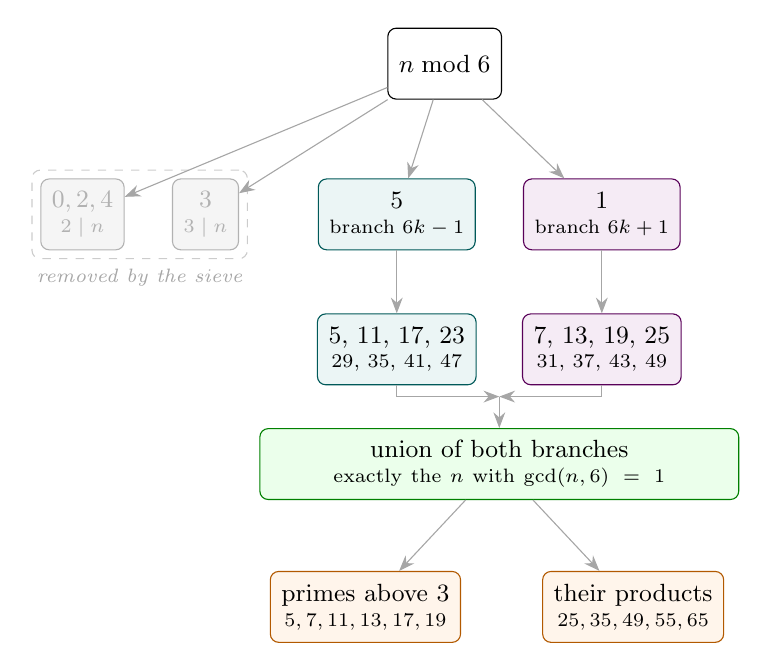
\begin{tikzpicture}[
  node distance = 8mm and 6mm,
  every node/.style = {font=\small},
  box/.style   = {draw, rounded corners=3pt, align=center,
                  inner sep=4pt, minimum height=9mm, line width=0.4pt},
  dead/.style  = {box, fill=gray!8,     draw=gray!60,    text=gray!60},
  minus/.style = {box, fill=teal!8,     draw=teal!70!black},
  plus/.style  = {box, fill=violet!8,   draw=violet!70!black},
  uni/.style   = {box, fill=green!8,    draw=green!50!black},
  leaf/.style  = {box, fill=orange!8,   draw=orange!70!black},
  ar/.style    = {-{Stealth[length=2mm]}, line width=0.4pt, gray!70}
]

\node[box] (root) {$n \bmod 6$};

\node[dead,  below=10mm of root, xshift=-46mm] (even)  {$0,2,4$\\[-2pt]\scriptsize $2 \mid n$};
\node[dead,  right=of even]                    (three) {$3$\\[-2pt]\scriptsize $3 \mid n$};
\node[minus, right=10mm of three]              (m)     {$5$\\[-2pt]\scriptsize branch $6k-1$};
\node[plus,  right=of m]                       (p)     {$1$\\[-2pt]\scriptsize branch $6k+1$};

\draw[ar] (root) -- (even);
\draw[ar] (root) -- (three);
\draw[ar] (root) -- (m);
\draw[ar] (root) -- (p);

\node[minus, below=8mm of m] (mex)
  {$5,\,11,\,17,\,23$\\[-2pt]\scriptsize $29,\,35,\,41,\,47$};
\node[plus,  below=8mm of p] (pex)
  {$7,\,13,\,19,\,25$\\[-2pt]\scriptsize $31,\,37,\,43,\,49$};

\draw[ar] (m) -- (mex);
\draw[ar] (p) -- (pex);

\node[uni, below=10mm of $(mex)!0.5!(pex)$, text width=58mm] (union)
  {union of both branches\\[-2pt]\scriptsize exactly the $n$ with $\gcd(n,6)=1$};

\draw[ar] (mex) |- ([yshift=4mm]union.north);
\draw[ar] (pex) |- ([yshift=4mm]union.north);
\draw[ar] ([yshift=4mm]union.north) -- (union.north);

\node[leaf, below=9mm of union, xshift=-17mm] (pr)
  {primes above $3$\\[-2pt]\scriptsize $5,7,11,13,17,19$};
\node[leaf, below=9mm of union, xshift=17mm]  (co)
  {their products\\[-2pt]\scriptsize $25,35,49,55,65$};

\draw[ar] (union) -- (pr);
\draw[ar] (union) -- (co);

\begin{scope}[on background layer]
  \node[draw=gray!40, dashed, rounded corners=3pt, inner sep=3pt,
        fit=(even)(three), label={[font=\scriptsize\itshape, text=gray!70]
        below:removed by the sieve}] {};
\end{scope}

\end{tikzpicture}
\caption{The residues modulo six. Four classes are eliminated by
divisibility by $2$ or $3$; the two survivors are the branches
$\mathcal{B}^-$ and $\mathcal{B}^+$, whose disjoint union is exactly
$\{n : \gcd(n,6)=1\}$ — the primes above $3$ together with all their
products.}
\label{fig:branches}
\end{figure}
\subsection{Contents of the union}

\begin{proposition}[Primes lie on the branches]
Every prime $p>3$ belongs to $\mathcal{B}$.
\end{proposition}

\begin{proof}
If $p \notin \mathcal{B}$ then by Theorem~\ref{thm:branches} either $2 \mid p$
or $3 \mid p$, contradicting primality for $p>3$.
\end{proof}

\begin{proposition}[Closure under multiplication]\label{prop:closure}
$\mathcal{B} \cup \{1\}$ is closed under multiplication, with the sign rule
\[
  \varepsilon(mn) = \varepsilon(m)\,\varepsilon(n),
  \qquad \varepsilon(6k\pm1) := \pm 1 .
\]
Explicitly,
\[
  (6a-1)(6b-1) = 6(6ab-a-b)+1, \quad
  (6a-1)(6b+1) = 6(6ab+a-b)-1, \quad
  (6a+1)(6b+1) = 6(6ab+a+b)+1 .
\]
\end{proposition}

\begin{corollary}[Branch group]
The map $\varepsilon : \mathcal{B} \to \{\pm 1\}$ is a surjective group
homomorphism from $(\mathbb{Z}/6\mathbb{Z})^{\times}$ onto
$\mathbb{Z}/2\mathbb{Z}$; the branches are its two cosets. Consequently a
product stays on the lower branch if and only if an odd number of its factors
lie there.
\end{corollary}

\begin{proposition}[The union is not the set of primes]
$\mathcal{B}$ contains every prime above $3$ together with every product of
such primes, and nothing else. The smallest composite members are
\[
  25 = 5^2, \quad 35 = 5\cdot 7, \quad 49 = 7^2, \quad
  55 = 5 \cdot 11, \quad 65 = 5\cdot 13 .
\]
\end{proposition}

\begin{proof}
Containment of primes and of their products follows from the previous two
propositions. Conversely, if $n \in \mathcal{B}$ then no prime factor of $n$
is $2$ or $3$, so every prime factor exceeds $3$.
\end{proof}

\begin{remark}[What the branch does and does not decide]
Membership in $\mathcal{B}$ is decided by a single residue computation and is
therefore not a primality criterion: $35$ and $11$ both lie on
$\mathcal{B}^-$, and $25$ and $37$ both lie on $\mathcal{B}^+$. The branch
records the residue of $n$ modulo $6$, an additive datum, whereas primality is
multiplicative. This is the same separation formalised in
Lemma~\ref{lem:coprime} and Corollary~\ref{cor:negative}.
\end{remark}

\subsection{Branch transitions under the descent}

\begin{proposition}
Let $n = 6k+\varepsilon$ with $\varepsilon = \pm1$. The branch of $n$ is
determined by $\varepsilon$ alone and is independent of the branch of $k$;
indeed $k$ need not lie in $\mathcal{B}$ at all, since $k$ may be divisible by
$2$ or $3$.
\end{proposition}

\begin{example}
$41 = 6\cdot 7 - 1$ has $k = 7 \in \mathcal{B}^+$, while
$47 = 6 \cdot 8 - 1$ has $k = 8 \notin \mathcal{B}$. Both lie on
$\mathcal{B}^-$.
\end{example}

\begin{remark}
This is why the canonical algorithm strips factors of $2$ and $3$ from $k$
before recursing: the descent lands in $\mathbb{Z}_{>0}$, not in
$\mathcal{B}$, and only the atoms $2$ and $3$ restore it.
\end{remark}

\subsection{Primality as a syntactic property}

\begin{proposition}[Bracketed canonical form]
Modify the canonical form so that every prime atom is enclosed in
parentheses: $2 \mapsto \texttt{(2)}$, $3 \mapsto \texttt{(3)}$, and
$p \mapsto \texttt{(}\,2\!\cdot\!3\!\cdot\! k \pm 1\,\texttt{)}$ for $p>3$.
Then for every $n>1$,
\[
  n \text{ is composite}
  \quad\Longleftrightarrow\quad
  \text{the substring } \texttt{)*(} \text{ occurs in } \mathrm{rep}(n).
\]
\end{proposition}

\begin{proof}
By construction $\mathrm{rep}(n)$ is a product of one bracketed factor per
prime in the factorisation of $n$, joined by \texttt{*}. If $n$ is composite
there are at least two such factors, so a \texttt{*} occurs between a closing
and an opening bracket. If $n$ is prime there is exactly one factor, and the
only \texttt{*} characters occur strictly inside its brackets, where every
occurrence is preceded by a digit or a closing bracket of a strictly nested
subexpression at depth $\ge 1$. Hence no depth-zero \texttt{*} exists.
\end{proof}

\begin{remark}[Bracketing is required]
Without brackets on the atoms $2$ and $3$ the test fails: $15$ would render as
\texttt{3*(2*3-1)} and $9$ as \texttt{3*3}, neither containing \texttt{)*(}.
\end{remark}

\begin{remark}[Cost]
The test is $O(|\mathrm{rep}(n)|) = O(\log n)$ on a string already in hand.
It does not reduce the cost of \emph{obtaining} that string, which requires
the prime factorisation of $n$ and dominates. The proposition therefore
records that primality is syntactically visible in the notation, not that it
is cheaply decidable from $n$.
\end{remark}

\begin{lstlisting}[language=Python]
def rep(n):
    if n <= 3:
        return "(" + str(n) + ")"
    p = smallest_factor(n)
    if p != n:
        return rep(p) + "*" + rep(n // p)
    k, s = ((n+1)//6, "-") if (n+1) % 6 == 0 else ((n-1)//6, "+")
    core = "2*3" if k == 1 else f"2*3*{rep(k)}"
    return f"({core}{s}1)"

def is_prime_form(N):
    if N < 2:
        return f"{N} is neither"
    forms = rep(N)
    label = "not prime" if ")*(" in forms else "prime"
    return f"{label} = {forms} = {N}"
\end{lstlisting}

\begin{proposition}[Factor-free variant]
Replacing \texttt{smallest\_factor} by trial division against $2$ and $3$
alone yields a map $\mathrm{rep}_{\mathrm{fast}}$ that is well defined,
terminating, and correct in value: $\mathrm{rep}_{\mathrm{fast}}(n)$ evaluates
to $n$ for every $n \ge 1$, at cost $O(\log n)$. It is neither canonical nor a
primality indicator.
\end{proposition}

\begin{proof}
Termination and correctness are as in Theorem 3, with the descent
$n \mapsto k \approx n/6$ interleaved with division by $2$ and $3$.
Non-canonicity and the failure of the syntactic test follow from the single
example
\[
  \mathrm{rep}_{\mathrm{fast}}(25) = (2\cdot3\cdot(2)\cdot(2)+1),
\]
which has no depth-zero product yet $25 = 5^2$ is composite. The canonical
form is $(2\cdot3-1)\cdot(2\cdot3-1)$.
\end{proof}

\begin{remark}
The two variants isolate the cost precisely. The $\pm1$ descent is
$O(\log n)$ and requires no factorisation; the canonical form requires the
full factorisation of $n$; and the syntactic primality reading is a property
of the canonical form alone. No reorganisation transfers the reading to the
cheap variant, since by Lemma~\ref{lem:coprime} the descent is coprime to
every level below it.
\end{remark}

\section{Three levels of structural resolution}

The expression tree admits three construction rules, differing only in how
much multiplicative structure is exposed at each node. All three produce
expressions over the atoms $\{1,2,3\}$ that evaluate to $n$; they differ in
cost and in what the shape of the tree reveals.

\subsection{Level 1: blind descent}

\begin{definition}[Blind form]
Define $\mathrm{rep}_{\mathrm{fast}}$ by peeling factors of $2$ and $3$ and
otherwise applying the descent $n \mapsto (n \mp 1)/6$ with the sign forced by
$n \bmod 6$.
\end{definition}

\begin{proposition}
$\mathrm{rep}_{\mathrm{fast}}$ is total, terminating, and value-correct:
$\mathrm{parse}(\mathrm{rep}_{\mathrm{fast}}(n)) = n$ for all $n \ge 1$, at
cost $O(\log n)$ arithmetic operations. It exposes no multiplicative
structure beyond the primes $2$ and $3$.
\end{proposition}

\begin{proposition}[Bijectivity]\label{prop:bijective}
$\mathrm{rep}_{\mathrm{fast}}$ is a bijection between $\mathbb{Z}_{>0}$ and
its image. Consequently every function of the blind tree is a function of $n$,
and no rewriting of the tree can expose a factorisation that was not computed.
\end{proposition}

\begin{example}[The shapes coincide]\label{ex:coincide}
\[
  \mathrm{rep}_{\mathrm{fast}}(25) = (2\cdot3\cdot(2)\cdot(2)+1),
  \qquad
  \mathrm{rep}_{\mathrm{fast}}(37) = (2\cdot3\cdot(2)\cdot(3)+1).
\]
The two trees are isomorphic as shapes: a $+1$ node above a binary product of
atoms. Yet $25 = 5^2$ and $37$ is prime. No rewrite rule keyed on tree shape
can distinguish them.
\end{example}

\subsection{Level 2: cheap canonicalisation}

\begin{definition}[Peel set]
Fix a finite set $P = \{p_1 < \dots < p_r\}$ of primes and let $q$ denote the
least prime not in $P$. Define $\mathrm{can}_P$ by applying, at each node with
value $n$, the following tests in order, and recursing on the results:
\begin{enumerate}
  \item if $n$ is a perfect square, $n = m \cdot m$;
  \item if $n \equiv 5 \pmod 6$ and $n+1 = s^2$, then $n = (s-1)(s+1)$;
  \item if $n \pm 1 = s^m$ for some $m \ge 2$, apply the cyclotomic
        factorisation of $s^m \mp 1$ (into cyclotomic polynomials
        $\Phi_d(s)$, $d\mid m$);
  \item if $p \mid n$ for some $p \in P$ with $p \ne n$, split $n = p \cdot (n/p)$;
  \item otherwise emit $(2\cdot3\cdot \mathrm{can}_P(k) \pm 1)$.
\end{enumerate}
\end{definition}

\begin{theorem}[Cost and coverage]\label{thm:cheap}
$\mathrm{can}_P$ runs in $O(|P| \log n)$ arithmetic operations and is
value-correct for every $n$. Its output is canonical --- that is, the root
operation is a product exactly when $n$ is composite --- for every $n$ whose
least prime factor lies in $P$, and for every $n$ caught by rules 1--3. The
least $n$ for which $\mathrm{can}_P$ fails to be canonical is $q^2$.
\end{theorem}

\begin{proof}
Each test is $O(\log n)$: an integer square root, a bounded number of $m$-th
roots, and $|P|$ divisions. If the least prime factor $p$ of $n$ lies in $P$,
rule 4 fires and the root becomes a product. If $n$ is composite with least
prime factor $p \notin P$, then $n \ge p^2 \ge q^2$, and rules 1--4 all fail
for $n = q^2$ only if $q^2$ is not a perfect square --- which is false, so the
first genuine failure is the least composite with least factor $q$ that is not
a perfect power, namely $q \cdot q'$ for the next prime $q'$. Taking $n=q^2$
as the bound is therefore conservative and holds a fortiori.
\end{proof}

\begin{table}[htbp]
\centering
\caption{Coverage as the peel set grows.}
\begin{tabular}{lll}
\hline
Peel set $P$ & least omitted prime $q$ & first structural failure \\
\hline
$\{2,3\}$                    & $5$  & $5 \cdot 7 = 35$ \\
$\{2,3,5\}$                  & $7$  & $7 \cdot 11 = 77$ \\
$\{2,3,5,7,11,13\}$          & $17$ & $17 \cdot 19 = 323$ \\
$\{2,3,5,7,11,13,17,19\}$    & $23$ & $23 \cdot 29 = 667$ \\
$\{2,\dots,31\}$             & $37$ & $37 \cdot 41 = 1517$ \\
$\{2,\dots,p_r\}$            & $q$  & $q\,q'$ \\
\hline
\end{tabular}
\label{tab:coverage}
\end{table}

\begin{corollary}[Extensibility]
Adjoining a prime $p$ to $P$ costs one further division per node and moves the
first structural failure from $q\,q'$ to the corresponding product for the new
least omitted prime. Coverage therefore increases monotonically with $|P|$ and
may be pushed to any desired bound $B$ by taking
$P = \{p : p \le \sqrt{B}\}$, at cost $O(\sqrt{B}/\log B)$ divisions per node.
\end{corollary}

\begin{remark}[Rules 1--3 are unbounded]
Unlike rule 4, the first three tests are not tied to a finite set: they catch
every perfect square, every twin product $(s-1)(s+1)$, and every splitting
$s^m \pm 1$, at all magnitudes, in $O(\log n)$ time. Their density is thin ---
perfect powers are sparse --- but they contribute at every scale, whereas the
peel set contributes only below $q^2$.
\end{remark}

\subsection{Level 3: full canonical form}

\begin{proposition}
Taking $P$ to be all primes up to $\sqrt{n}$ recovers the canonical form of
Theorem \ref{thm:canonical}. The cost is that of trial division, $O(\sqrt{n})$,
or $O(n^{1/4})$ with Pollard's rho substituted for rule 4.
\end{proposition}

\subsection{Summary}

\begin{table}[htbp]
\centering
\caption{The three levels.}
\begin{tabular}{llll}
\hline
Level & Cost & Value & Structure \\
\hline
$\mathrm{rep}_{\mathrm{fast}}$ & $O(\log n)$        & exact & none beyond $2,3$ \\
$\mathrm{can}_P$               & $O(|P| \log n)$    & exact & exact below $q^2$ \\
$\mathrm{rep}$                 & $O(\sqrt{n})$      & exact & exact \\
\hline
\end{tabular}
\end{table}

\begin{remark}[Why the levels do not collapse]
The three functions agree on value and disagree only on structure, and the
disagreement is not removable by post-processing. By
Proposition~\ref{prop:bijective} the blind tree determines $n$ and nothing
more, and by Example~\ref{ex:coincide} it does not determine primality even
locally. Each additional prime admitted to $P$ purchases a bounded increment
of structural resolution at a bounded increment of cost; the limit of this
process is trial division. In this sense the three levels are not three
algorithms but one algorithm at three settings of a single parameter, and the
notation makes the trade-off between cost and resolution explicit rather than
implicit.
\end{remark}

\subsection{Implementation}

\begin{lstlisting}[language=Python]
from math import isqrt

def rep_fast(n):
    if n <= 3:
        return "(" + str(n) + ")"
    for d in (2, 3):
        if n % d == 0:
            return f"({d})*" + rep_fast(n // d)
    k, s = ((n+1)//6, "-") if (n+1) % 6 == 0 else ((n-1)//6, "+")
    core = "2*3" if k == 1 else f"2*3*{rep_fast(k)}"
    return f"({core}{s}1)"


def can_P(n, P=(2, 3, 5, 7, 11, 13, 17, 19, 23, 29, 31)):
    if n <= 3:
        return "(" + str(n) + ")"
    r = isqrt(n)
    if r * r == n:
        h = can_P(r, P)
        return h + "*" + h
    if n % 6 == 5:
        s = isqrt(n + 1)
        if s * s == n + 1:
            return can_P(s - 1, P) + "*" + can_P(s + 1, P)
    for d in P:
        if n != d and n % d == 0:
            return can_P(d, P) + "*" + can_P(n // d, P)
    k, s = ((n+1)//6, "-") if (n+1) % 6 == 0 else ((n-1)//6, "+")
    core = "2*3" if k == 1 else f"2*3*{can_P(k, P)}"
    return f"({core}{s}1)"


def smallest_factor(n):
    for d in (2, 3):
        if n % d == 0:
            return d
    k = 1
    while True:
        for d in (6*k - 1, 6*k + 1):
            if d * d > n:
                return n
            if n % d == 0:
                return d
        k += 1


def rep(n):
    if n <= 3:
        return "(" + str(n) + ")"
    p = smallest_factor(n)
    if p != n:
        return rep(p) + "*" + rep(n // p)
    k, s = ((n+1)//6, "-") if (n+1) % 6 == 0 else ((n-1)//6, "+")
    core = "2*3" if k == 1 else f"2*3*{rep(k)}"
    return f"({core}{s}1)"
\end{lstlisting}

\begin{proposition}[Agreement]
For all $n$, $\mathrm{parse}(f(n)) = n$ where $f$ is any of the three
functions. Moreover $\mathrm{can}_P(n) = \mathrm{rep}(n)$ whenever the least
prime factor of $n$ lies in $P$ or $n$ is caught by rules 1--3, and
$\mathrm{can}_{\varnothing}(n) = \mathrm{rep}_{\mathrm{fast}}(n)$ when rules
1--3 are also disabled.
\end{proposition}
\section{Generating Pythagorean partners from a fixed leg}

\subsection{The governing equations}

Fix a positive integer $A$ and seek all $B > A$ and $C > 0$ with
\begin{equation}\label{eq:pyth}
  B^2 - A^2 = C^2 .
\end{equation}
Writing $B = A + d$ for the gap $d = B - A$ and applying the gap identity of
Section 2,
\begin{equation}\label{eq:gap}
  B^2 - A^2 = 2Ad + d^2 = d\,(2A+d),
\end{equation}
so \eqref{eq:pyth} is equivalent to requiring $d\,(2A+d)$ to be a perfect
square. Equivalently, factoring the left side of \eqref{eq:pyth} as a
difference of two squares in the other pair of variables,
\begin{equation}\label{eq:factor}
  (B-C)(B+C) = A^2 .
\end{equation}

\begin{theorem}[Partner enumeration]\label{thm:partners}
The solutions $(B,C)$ of \eqref{eq:pyth} in positive integers are in bijection
with the factorisations
\[
  A^2 = d\,e, \qquad d < e, \qquad d \equiv e \pmod 2,
\]
the correspondence being
\begin{equation}\label{eq:solve}
  B = \frac{d+e}{2}, \qquad C = \frac{e-d}{2},
\end{equation}
with inverse $d = B-C$, $e = B+C$.
\end{theorem}

\begin{proof}
Given such a factorisation, \eqref{eq:solve} produces integers because
$d \equiv e \pmod 2$, and
\[
  B^2 - C^2 = \Bigl(\tfrac{d+e}{2}\Bigr)^{2} - \Bigl(\tfrac{e-d}{2}\Bigr)^{2}
            = de = A^2 ,
\]
so \eqref{eq:pyth} holds; $C>0$ follows from $d<e$. Conversely, given a
solution, set $d = B-C$ and $e = B+C$. Then $de = A^2$ by \eqref{eq:factor},
$d<e$ since $C>0$, and $d+e = 2B$ is even, so $d \equiv e \pmod 2$. The two
maps are mutually inverse.
\end{proof}

\begin{corollary}[Parity]
If $A$ is odd then $A^2$ is odd, so $d$ and $e$ are both odd and the parity
condition is automatic. If $A$ is even then $4 \mid A^2$ and the admissible
factorisations are those with both parts even.
\end{corollary}

\begin{corollary}[Count]\label{cor:count}
The number of partners of $A$ equals the number of admissible factorisations
of $A^2$, hence is governed by $\tau(A^2)$. In particular, if $A$ is an odd
prime then $A^2 = 1 \cdot A^2$ is the only admissible factorisation and $A$ has
the unique partner
\[
  B = \frac{A^2+1}{2}, \qquad C = \frac{A^2-1}{2}.
\]
\end{corollary}

\begin{example}
$\mathrm{partners}(11)$ returns $\{(61,60)\}$, since $11$ is prime; whereas
$\mathrm{partners}(15)$ returns
$\{(113,112),\,(39,36),\,(25,20),\,(17,8)\}$, corresponding to the
factorisations $225 = 1\cdot225 = 3\cdot75 = 5\cdot45 = 9\cdot25$.
\end{example}

\begin{remark}
Corollary~\ref{cor:count} shows that the partner count of $A$ is a disguised
divisor count: the multiplicative structure of $A$ is read off directly from
the number of right triangles admitting $A$ as a leg.
\end{remark}

\subsection{Conversion to sums of two squares}

\begin{proposition}\label{prop:sumdiff}
For integers $p,q,n$,
\[
  p^2 + q^2 = n^2
  \iff
  (p-q)^2 + (p+q)^2 = 2n^2 .
\]
\end{proposition}

\begin{proof}
Expand: $(p-q)^2+(p+q)^2 = 2p^2+2q^2$.
\end{proof}

Since Theorem~\ref{thm:partners} enumerates triples by leg, and
Proposition~\ref{prop:sumdiff} converts a triple with hypotenuse $n$ into a
representation $2n^2 = x^2+y^2$, iterating \texttt{partners} over all legs
$\le N$ and indexing the results by the hypotenuse $B$ yields, for every
$n \le N$, the complete list of such representations. Centres admitting
several representations are exactly those $n$ divisible by sufficiently many
primes congruent to $1 \bmod 4$.

\subsection{Implementation}

\begin{lstlisting}[language=Python]
def partners(A):
    """All (B, C) with B^2 - A^2 = C^2."""
    out = []
    n = A * A
    d = 1
    while d * d < n:
        if n % d == 0:
            e = n // d
            if (d + e) % 2 == 0:          # both same parity
                B, C = (d + e) // 2, (e - d) // 2
                if C > 0:
                    out.append((B, C))
        d += 1
    return out
\end{lstlisting}

The loop condition $d^2 < n$ enumerates the smaller part of each factorisation
of $n = A^2$, so each pair $\{d,e\}$ is visited once and $d<e$ holds
throughout; the parity test implements the congruence of
Theorem~\ref{thm:partners}, and the assignments are \eqref{eq:solve} verbatim.
The cost is $O(A)$ divisions, since $d$ ranges up to $\sqrt{A^2} = A$.

%==================================================================
\section{Background: the mod-6 wheel}
%==================================================================

Every integer occupies one of six lanes modulo $6$. Lanes
$0,2,4$ are even and lane $3$ is divisible by $3$, so beyond the base
primes $2$ and $3$ only lanes $1$ and $5$ can hold primes:
\[
p > 3 \;\Longrightarrow\; p \equiv 1 \text{ or } 5 \pmod 6,
\qquad\text{i.e.}\qquad p = 6m \pm 1 .
\]
These two survivors are exactly the fold (reset) positions of the two
sawtooth waves
\[
B = \bigl((x - \tfrac{6}{8}) \bmod 6\bigr)\cdot 2,
\qquad
D = \bigl((x + 2 - \tfrac{6}{8}) \bmod 6\bigr)\cdot 2 ,
\]
which reset at $x \bmod 6 = 1$ and $x \bmod 6 = 5$ respectively.

%==================================================================
\section{Base-60 inheritance}
%==================================================================

Base $60$ factors as $60 = 6 \times 10$: a mod-$6$ ``tens'' wheel geared to
a base-$10$ ``units'' wheel. We compute in base $10$ but time and angle
keep the base-$60$ rollover, whose reset is precisely the $x \bmod 6 = 5$
event of the wheel above. The sieving power of $60$ lives entirely in its
squarefree kernel $30 = 2\cdot 3\cdot 5$.

%==================================================================
\section*{\textbf{Details: The Totient Relation}}
\addcontentsline{toc}{section}{Details: The Totient Relation}
%==================================================================
\markboth{Details: The Totient Relation}{}

Euler's totient $\varphi$ is the hinge of this entire construction. It
appears in \emph{two} distinct roles: once attached to the wheel modulus
$M$, and once attached to the integer $N$ under test.

\begin{definition}[Totient]
For a positive integer $n$,
\[
\varphi(n) \;=\; \bigl|\{\, k : 1 \le k \le n,\ \gcd(k,n)=1 \,\}\bigr|,
\]
the count of integers up to $n$ that are coprime to $n$.
\end{definition}

\subsection*{Role 1 --- $\varphi(M)$ is the wheel width}

For a wheel with modulus $M$, the spokes are exactly the residues coprime
to $M$, so the number of spokes is $\varphi(M)$ and the surviving density
of the number line is $\varphi(M)/M$. This density is governed by the
multiplicative product formula.

\begin{theorem}[Euler product formula]
\[
\varphi(M) \;=\; M \prod_{p \mid M} \Bigl(1 - \frac{1}{p}\Bigr),
\]
the product ranging over the \emph{distinct} primes dividing $M$.
Consequently the wheel density is
\[
\frac{\varphi(M)}{M} \;=\; \prod_{p \mid M}\Bigl(1 - \frac1p\Bigr).
\]
\end{theorem}

Each factor $(1-1/p)$ is one prime's worth of lanes struck out. This one
equation explains every empirical observation about the wheels:

\begin{center}
\begin{tabular}{r r c c l}
\toprule
$M$ & $\varphi(M)$ & $\varphi(M)/M$ & $\prod(1-1/p)$ & distinct primes of $M$\\
\midrule
$6$    & $2$   & $0.3333$ & $0.3333$ & $\{2,3\}$\\
$30$   & $8$   & $0.2667$ & $0.2667$ & $\{2,3,5\}$\\
$60$   & $16$  & $0.2667$ & $0.2667$ & $\{2,3,5\}$ \quad(no gain over $30$)\\
$210$  & $48$  & $0.2286$ & $0.2286$ & $\{2,3,5,7\}$\\
$2310$ & $480$ & $0.2078$ & $0.2078$ & $\{2,3,5,7,11\}$\\
\bottomrule
\end{tabular}
\end{center}

\noindent Two consequences follow immediately:
\begin{itemize}
  \item \textbf{$60$ gains nothing over $30$:} they share the distinct
        primes $\{2,3,5\}$, so the product---and hence the density---is
        identical. The extra factor of $2$ in $60=2^2\cdot3\cdot5$ never
        enters the product, which counts only \emph{distinct} primes.
  \item \textbf{$210$ does gain:} it introduces a genuinely new factor
        $(1-1/7)$, lowering the density from $0.2667$ to $0.2286$.
\end{itemize}

\subsection*{Role 2 --- $\varphi(N)$ is a primality signature}

For the integer $N$ passed to the scan, the totient encodes primality
directly:
\[
N \text{ is prime} \;\Longleftrightarrow\; \varphi(N) = N-1,
\qquad\qquad
\varphi(p^k) = p^k - p^{k-1}.
\]
A prime shares a factor with nothing below it, so all $N-1$ smaller
integers are coprime---the maximal possible totient. Every composite
satisfies $\varphi(N) < N-1$.

\subsection*{The bridge --- Euler's theorem}

The two roles are joined by Euler's theorem, which also underlies the
fast primality tests (Fermat, Miller--Rabin) that outperform trial
division for large $N$.

\begin{theorem}[Euler]
If $\gcd(a,N)=1$ then
\[
a^{\varphi(N)} \equiv 1 \pmod{N}.
\]
For prime $p$ this specialises, via $\varphi(p)=p-1$, to Fermat's little
theorem $a^{\,p-1}\equiv 1 \pmod p$.
\end{theorem}

Miller--Rabin checks whether $N$ \emph{violates} this congruence: a
violation certifies compositeness with a single modular exponentiation,
whereas the wheel must trial-divide up to $\sqrt N$.

\subsection*{Summary}

\[
\boxed{\;
\underbrace{\varphi(M)}_{\text{sieve width}}
\;=\; M\!\prod_{p\mid M}\!\Bigl(1-\tfrac1p\Bigr)
\qquad\text{and}\qquad
\underbrace{\varphi(N)=N-1}_{\text{primality signature}}
\;\Longleftrightarrow\; N \text{ prime},
\;}
\]
the same function serving once as a wheel's width and once as an integer's
primality signature, bridged by $a^{\varphi(N)}\equiv 1 \pmod N$.

%==================================================================
\section{Reference implementation}
%==================================================================

The mod-$210$ wheel ($210 = 2\cdot3\cdot5\cdot7$, $\varphi(210)=48$ spokes)
used as a trial-division primality scanner:

\begin{lstlisting}
from math import gcd, isqrt

WHEEL210 = [r for r in range(210) if gcd(r, 210) == 1]   # 48 spokes

def wheel_scan_210(N):
    """Smallest factor of N via a mod-210 wheel, or None if N is prime."""
    if N < 2:
        return None
    for p in (2, 3, 5, 7):            # base primes the wheel skips
        if N == p:  return None
        if N % p == 0: return p
    limit = isqrt(N)
    m = 0
    while 210*m + 1 <= limit:
        for r in WHEEL210:
            n = 210*m + r             # actual candidate = block offset + spoke
            if n == 1:                # skip trivial divisor
                continue
            if n > limit:
                break
            if N % n == 0:
                return n              # real factor -> composite
        m += 1
    return None                       # nothing up to sqrt(N) -> prime

def is_prime(N):
    return N >= 2 and wheel_scan_210(N) is None
\end{lstlisting}

\section{The period-six sawtooth and its fold}

The trichotomy modulo six can be read dynamically. Writing $6/8=0.75$, define
the two phase-shifted waves
\[
  B(x) = \bigl((x - \tfrac{6}{8}) \bmod 6\bigr)\cdot 2,
  \qquad
  D(x) = \bigl((x + 2 - \tfrac{6}{8}) \bmod 6\bigr)\cdot 2 .
\]

\begin{proposition}[Shape and phase]
Both $B$ and $D$ are sawtooths of period $6$, and $D(x)=B(x+2)$; that is, $D$ is
$B$ advanced by two steps. On integer arguments each takes the half-integer
values $\{0.5,2.5,4.5,6.5,8.5,10.5\}$, never landing on an integer.
\end{proposition}

\begin{proof}
Periodicity and the identity $D(x)=B(x+2)$ are immediate from the definitions,
since $x+2-\tfrac68 = (x+2)-\tfrac68$. For integer $x$ the argument
$x-\tfrac68$ has fractional part $0.25$, so $(x-\tfrac68)\bmod 6 \in
\{0.25,1.25,\dots,5.25\}$ and multiplication by $2$ gives the stated
half-integers. The offset $\tfrac68=\tfrac34$ keeps every output off the
integer grid, so the wrap point is unambiguous.
\end{proof}

\begin{proposition}[The fold locates the residue]
$D$ attains its minimum exactly when $x\equiv 5\pmod 6$, and $B$ attains its
minimum exactly when $x\equiv 1\pmod 6$. Equivalently
\[
  x \equiv 5 \pmod 6 \iff D(x)=0.5, \qquad
  x \equiv 1 \pmod 6 \iff B(x)=0.5 .
\]
\end{proposition}

\noindent The reset (maximum $\to$ minimum) of each wave marks the residue where
it folds. Because $D=B(\cdot+2)$, the two folds sit at the residues $1$ and $5$
--- precisely the two lanes coprime to six of the Trichotomy proposition, and
hence the only lanes a prime $>3$ may occupy.

\begin{center}
\begin{tabular}{c c c c}
\hline
$x\bmod 6$ & $B$ & $D$ & note\\
\hline
$0$ & $10.5$ & $2.5$  & \\
$1$ & $0.5$  & $4.5$  & $B$ resets (prime lane)\\
$2$ & $2.5$  & $6.5$  & \\
$3$ & $4.5$  & $8.5$  & \\
$4$ & $6.5$  & $10.5$ & $D$ peaks\\
$5$ & $8.5$  & $0.5$  & $D$ resets $=x\equiv5$ (prime lane)\\
\hline
\end{tabular}
\end{center}

\section{Base-sixty inheritance}

The wheel of six is inherited by the sexagesimal systems still used for time and
angle. The factorisation
\[
  60 = 6 \times 10
\]
gears a mod-$6$ ``tens'' wheel to a base-$10$ ``units'' wheel: a value $v$ with
$0\le v<60$ decomposes as
\[
  v = 10\,t + u, \qquad t=\Bigl\lfloor \tfrac{v}{10}\Bigr\rfloor \in\{0,\dots,5\},
  \quad u = v \bmod 10 \in \{0,\dots,9\}.
\]

\begin{center}
\begin{tabular}{c|cccccccccc}
$t\backslash u$ & 0&1&2&3&4&5&6&7&8&9\\
\hline
0 & 0&1&2&3&4&5&6&7&8&9\\
1 & 10&11&12&13&14&15&16&17&18&19\\
2 & 20&21&22&23&24&25&26&27&28&29\\
3 & 30&31&32&33&34&35&36&37&38&39\\
4 & 40&41&42&43&44&45&46&47&48&49\\
5 & 50&51&52&53&54&55&56&57&58&59\\
\end{tabular}
\end{center}

\begin{remark}[The fold at one half, and the effect of the zero]
The tens wheel is capped at $5$, the midpoint $5/10=\tfrac12$ of a decimal
digit; its top half $\{6,7,8,9\}$ is never used. This ``fold at one half'' is an
artefact of zero-based indexing: the wheel \emph{counts} six states $\{0,\dots,5\}$
but \emph{folds} at position $5$, the usual gap between an index and a count.
If the system omits zero and runs $1,\dots,6$ instead, index and count coincide:
the value is $((x-1)\bmod 6)+1$, the fold moves to $6$, and the reset condition
changes from $x\equiv 5$ to $x\equiv 0 \pmod 6$ (the multiples of six). The
sieving power of $60$ resides entirely in its squarefree kernel
$30 = 2\cdot 3\cdot 5$; the extra factor of $2$ in $60=2^2\cdot3\cdot5$ adds no
new prime.
\end{remark}

\section{Wheel factorisation and the totient density}

The $6k\pm1$ enumeration is the wheel of modulus $6$. Replacing $6$ by a general
modulus $M$ and keeping only the residues coprime to $M$ yields a wheel with
$\varphi(M)$ spokes, where $\varphi$ is Euler's totient. The modulus $210 =
2\cdot3\cdot5\cdot7$ gives $\varphi(210)=48$ spokes and, used as a trial-division
scanner, tests $N$ against the base primes $\{2,3,5,7\}$ and then the wheel
candidates up to $\sqrt N$.

\begin{lstlisting}[language=Python]
from math import gcd, isqrt

WHEEL210 = [r for r in range(210) if gcd(r, 210) == 1]   # 48 spokes

def wheel_scan_210(N):
    """Smallest factor of N via a mod-210 wheel, or None if N is prime."""
    if N < 2:
        return None
    for p in (2, 3, 5, 7):            # base primes the wheel skips
        if N == p:  return None
        if N % p == 0: return p
    limit = isqrt(N)
    m = 0
    while 210*m + 1 <= limit:
        for r in WHEEL210:
            n = 210*m + r             # candidate = block offset + spoke
            if n == 1:                # skip the trivial divisor
                continue
            if n > limit:
                break
            if N % n == 0:
                return n              # real factor -> composite
        m += 1
    return None                       # nothing up to sqrt(N) -> prime

def is_prime(N):
    return N >= 2 and wheel_scan_210(N) is None
\end{lstlisting}

\noindent The three critical corrections over a naive version are: dividing by
the actual candidate $n=Mm+r$ rather than the residue $r$; skipping $n=1$, which
would otherwise divide every $N$; and testing the base primes separately, since
the wheel omits them. The scan runs in $O(\sqrt N)$ divisions scaled by the
survivor density $\varphi(M)/M$.

\section{The totient relation}

Euler's totient $\varphi$ enters this construction in two distinct roles: once
attached to the wheel modulus $M$, and once attached to the integer $N$ under
test.

\begin{definition}[Totient]
For a positive integer $n$,
$\varphi(n)=\bigl|\{k:1\le k\le n,\ \gcd(k,n)=1\}\bigr|$, the count of integers
up to $n$ coprime to $n$.
\end{definition}

\begin{theorem}[Sieve width]\label{thm:sievewidth}
A wheel of modulus $M$ has exactly $\varphi(M)$ spokes, and the fraction of the
integers it retains is
\[
  \frac{\varphi(M)}{M} \;=\; \prod_{p\mid M}\Bigl(1-\frac1p\Bigr),
\]
the product over the distinct primes dividing $M$.
\end{theorem}

Each factor $(1-1/p)$ removes one prime's lanes. The formula explains the
observed densities:

\begin{center}
\begin{tabular}{r r c c l}
\hline
$M$ & $\varphi(M)$ & $\varphi(M)/M$ & $\prod(1-1/p)$ & distinct primes\\
\hline
$6$    & $2$   & $0.3333$ & $0.3333$ & $\{2,3\}$\\
$30$   & $8$   & $0.2667$ & $0.2667$ & $\{2,3,5\}$\\
$60$   & $16$  & $0.2667$ & $0.2667$ & $\{2,3,5\}$ (no gain over $30$)\\
$210$  & $48$  & $0.2286$ & $0.2286$ & $\{2,3,5,7\}$\\
$2310$ & $480$ & $0.2078$ & $0.2078$ & $\{2,3,5,7,11\}$\\
\hline
\end{tabular}
\end{center}

\noindent Thus $60$ yields no improvement over $30$ (identical distinct primes),
whereas $210$ tightens the sieve by folding in the new factor $(1-1/7)$.

\begin{proposition}[Primality signature]
For the integer $N$ under test, $N$ is prime iff $\varphi(N)=N-1$, and
$\varphi(p^k)=p^k-p^{k-1}$.
\end{proposition}

\begin{theorem}[Euler, the bridge]
If $\gcd(a,N)=1$ then $a^{\varphi(N)}\equiv 1 \pmod N$. For prime $p$ this
reduces, via $\varphi(p)=p-1$, to Fermat's little theorem
$a^{\,p-1}\equiv 1 \pmod p$.
\end{theorem}

The two roles are the same function seen twice: $\varphi(M)$ as the width of the
sieve (Theorem~\ref{thm:sievewidth}) and $\varphi(N)=N-1$ as the signature of
primality, joined by Euler's congruence, which is the basis of the fast tests
(Fermat, Miller--Rabin) that supersede trial division for large $N$.

\section{Details: reciprocity of the sieve factor and the base-\texorpdfstring{$p$}{p} expansion}

The wheel multiplies the factors $(1-1/p)$; the complementary object is their
reciprocal, the base-$p$ geometric series. The two are related by a single
inverse identity, which the following floating-point experiment exhibits in
base $2$.

\begin{lstlisting}[language=Python]
for x in range(2, 100):
    A = ((x + (1/x)) % x)
    if (x*A % x) == 1.0:
        print(x, (x*A % x))
# printed:  2, 4, 8, 16, 32, 64
\end{lstlisting}

\begin{proposition}[What the loop computes]
For every integer $x\ge 2$ one has $A=(x+1/x)\bmod x = 1/x$, hence
$x\cdot A = 1$ and $(x\cdot A)\bmod x = 1$. In exact arithmetic the test
$x\cdot A = 1$ therefore holds for \emph{all} $x$: it is the multiplicative
inverse identity $x\cdot(1/x)=1$.
\end{proposition}

\begin{remark}[Why only the powers of two are printed]
The equality is with the literal $1.0$ in IEEE-754 double precision, which is
base $2$. The reciprocal $1/x$ is represented \emph{exactly} only when
$x=2^{J}$, since then $1/x=2^{-J}$ is a finite binary fraction; the round-trip
$(x+1/x)\bmod x$ then returns exactly $2^{-J}$ and $x\cdot A$ is exactly $1.0$.
For any other $x$ the product rounds to $1.0\pm\varepsilon$ and fails the test.
Thus the loop is, in effect, a detector of the powers of two --- the base-$2$
signature.
\end{remark}

\begin{proposition}[Sieve factor and base-$p$ series are reciprocal]
For every prime $p$,
\[
  \frac{1}{1-\tfrac1p}
  \;=\; \sum_{J\ge 0} \frac{1}{p^{J}}
  \;=\; 1+\frac1p+\frac1{p^{2}}+\cdots,
  \qquad\text{so}\qquad
  \Bigl(1-\tfrac1p\Bigr)\cdot\sum_{J\ge 0}\frac{1}{p^{J}} = 1 .
\]
\end{proposition}

\noindent This is the local Euler factor of the Riemann product
$\zeta(s)=\prod_p (1-p^{-s})^{-1}$ at $s=1$. The sieve factor $(1-1/p)$ measures
what \emph{survives} the wheel (the lanes coprime to $p$); its reciprocal
$\sum_J p^{-J}$ \emph{generates} what the wheel removes (the powers and multiples
of $p$). Their product is $1$ --- the same inverse identity $x\cdot(1/x)=1$ that
the loop tests.

\begin{center}
\begin{tabular}{c c c c}
\hline
$p$ & $1-1/p$ (sieve) & $1/(1-1/p)=\sum_J p^{-J}$ & product\\
\hline
$2$ & $0.5000$ & $2.0000=\sum_J 2^{-J}$ & $1$\\
$3$ & $0.6667$ & $1.5000$ & $1$\\
$5$ & $0.8000$ & $1.2500$ & $1$\\
$7$ & $0.8571$ & $1.1667$ & $1$\\
\hline
\end{tabular}
\end{center}

\noindent For $p=2$ the reciprocal series is the geometric expansion
\[
  \frac{1}{1-\tfrac12} \;=\; \sum_{J\ge 0}\frac{1}{2^{J}}
  \;=\; 1+\tfrac12+\tfrac14+\tfrac18+\cdots \;=\; 2,
\]
the exact $2^{J}$ series of the loop and the reciprocal of the wheel's smallest
factor $(1-\tfrac12)$. Because floating-point arithmetic is itself base $2$, this
is the one Euler factor the machine represents exactly, which is why the
inverse test $x\cdot(1/x)=1$ selects precisely the powers of two. In summary,
\[
  \underbrace{\prod_p\Bigl(1-\tfrac1p\Bigr)}_{\text{wheel: keeps coprimes}}
  \qquad\text{and}\qquad
  \underbrace{\prod_p \frac{1}{1-\tfrac1p}=\prod_p\sum_{J\ge0}p^{-J}}_{\text{base-}p\text{ generator}}
\]
are reciprocal expressions of the same primes, meeting at $x\cdot(1/x)=1$.

\section{The square-root staircase}

Pairing the inverse identity of the previous section with the integer square
root exposes a second structure: a step function whose runs are the odd numbers.

\begin{lstlisting}[language=Python]
from math import isqrt
for x in range(3, 100):
    A  = ((x  + 1/x ) % x )     # = 1/x   -> x*A % x  approx 1.0
    x1 = isqrt(x)               # the "category" floor(sqrt(x))
    A1 = ((x1 + 1/x1) % x1)     # = 1/x1  -> x1*A1 % x1 approx 1.0
    print(x, (x*A % x), x1, (x1*A1 % x1))
\end{lstlisting}

The two remainder columns are both the constant $\approx 1$ of the identity
$x\cdot(1/x)=1$; the information is carried entirely by $x_1=\lfloor\sqrt x\rfloor$,
a staircase that is flat on each block and steps up by one at every perfect
square.

\begin{proposition}[Odd-length runs]
Fix $k\ge 1$. Then $\lfloor\sqrt x\rfloor = k$ precisely for
$k^{2}\le x \le (k+1)^{2}-1$, a run of length
\[
  (k+1)^{2}-k^{2} \;=\; 2k+1 .
\]
Consequently the gaps between consecutive squares are the odd numbers, and
\[
  k^{2} \;=\; 1+3+5+\cdots+(2k-1) \;=\; \sum_{j=1}^{k}(2j-1).
\]
\end{proposition}

\begin{proof}
$\lfloor\sqrt x\rfloor = k \iff k \le \sqrt x < k+1 \iff k^{2}\le x <(k+1)^{2}$,
so the run is the integer interval $[k^{2},(k+1)^{2}-1]$ of length
$(k+1)^{2}-k^{2}=2k+1$. Summing these increments telescopes:
$\sum_{j=1}^{k}(2j-1)=k^{2}$.
\end{proof}

\begin{center}
\begin{tabular}{c c c c}
\hline
$k=\lfloor\sqrt x\rfloor$ & $x$ range & run length & $(k+1)^2-k^2$\\
\hline
$4$ & $16\ldots24$ & $9$  & $9$\\
$5$ & $25\ldots35$ & $11$ & $11$\\
$6$ & $36\ldots48$ & $13$ & $13$\\
$7$ & $49\ldots63$ & $15$ & $15$\\
$8$ & $64\ldots80$ & $17$ & $17$\\
\hline
\end{tabular}
\end{center}

\noindent The category $k$ persists for exactly $2k+1$ consecutive integers,
turning over only at the boundary squares $k^{2}$. The square numbers are the
partial sums of the odd numbers, and $\lfloor\sqrt x\rfloor$ is the step
function counting which shell $x$ occupies.

\subsection{Connection to the divisor bound and to differences of squares}

The staircase links two earlier constructions.

\begin{remark}[Trial-division bound]
In the wheel scan the search is capped at $\texttt{limit}=\lfloor\sqrt N\rfloor$.
For all $x$ in one run of the staircase, $\sqrt x$ lies in the same integer shell
$[k,k+1)$; the ``category'' is precisely the divisor bound below which a factor,
if any, must appear.
\end{remark}

\begin{remark}[Fermat descent walks the staircase]
The difference-of-squares identity $n=a^{2}-b^{2}=(a-b)(a+b)$ is searched by
starting at $a=\lfloor\sqrt n\rfloor$ and increasing $a$, testing whether
$a^{2}-n$ is a perfect square. Each increment raises $a^{2}$ by the odd number
$2a+1$, so Fermat's method advances exactly along the square staircase of the
proposition; the odd-gap law is its step size.
\end{remark}

\subsection{Higher power staircases}

Nesting the integer square root raises the staircase one level up the power
ladder. Since the nested floors collapse,
\[
  \bigl\lfloor \sqrt{\lfloor \sqrt x\rfloor}\,\bigr\rfloor
  \;=\; \bigl\lfloor x^{1/4}\bigr\rfloor,
\]
the double root \texttt{isqrt(isqrt(x))} is the integer fourth root, constant
between consecutive fourth powers and stepping at $16,81,256,625,\dots$

\begin{lstlisting}[language=Python]
from math import isqrt
for x in range(4, 100):
    A  = ((x  + 1/x ) % x )
    x1 = isqrt(isqrt(x))        # integer 4th root: floor(x**(1/4))
    A1 = ((x1 + 1/x1) % x1)
    print(x, (x*A % x), x1, (x1*A1 % x1))
\end{lstlisting}

\begin{proposition}[Fourth-power runs]
$\lfloor x^{1/4}\rfloor = k$ precisely for $k^{4}\le x\le(k+1)^{4}-1$, a run of
length
\[
  (k+1)^{4}-k^{4} \;=\; 4k^{3}+6k^{2}+4k+1 .
\]
\end{proposition}

\begin{center}
\begin{tabular}{c c c c}
\hline
$k=\lfloor x^{1/4}\rfloor$ & $x$ range & run length & $(k+1)^4-k^4$\\
\hline
$1$ & $1\ldots15$   & $15$  & $15$\\
$2$ & $16\ldots80$  & $65$  & $65$\\
$3$ & $81\ldots255$ & $175$ & $175$\\
\hline
\end{tabular}
\end{center}

\noindent The run for $k=2$ is exactly $3^{4}-2^{4}=81-16=65$.

\begin{theorem}[Binomial gap law]\label{thm:gaplaw}
For each integer $m\ge 1$, the map $x\mapsto\lfloor x^{1/m}\rfloor$ is constant
on $[k^{m},(k+1)^{m}-1]$, and the length of that run is the discrete derivative
of $k^{m}$:
\[
  (k+1)^{m}-k^{m} \;=\; \sum_{j=0}^{m-1}\binom{m}{j}k^{j}.
\]
The coefficients are row $m$ of Pascal's triangle with the leading $k^{m}$ term
removed.
\end{theorem}

\begin{proof}
$\lfloor x^{1/m}\rfloor=k \iff k^{m}\le x<(k+1)^{m}$, giving the stated interval
and length $(k+1)^{m}-k^{m}$. The binomial theorem expands
$(k+1)^{m}=\sum_{j=0}^{m}\binom{m}{j}k^{j}$; subtracting the $j=m$ term $k^{m}$
leaves $\sum_{j=0}^{m-1}\binom{m}{j}k^{j}$.
\end{proof}

\noindent The earlier square-root staircase is the case $m=2$, whose gap
$2k+1$ is the odd numbers (Pascal row $2$); the fourth root is $m=4$, gap
$4k^{3}+6k^{2}+4k+1$ (row $4$: $1,4,6,4,1$). Each further nesting of
\texttt{isqrt} doubles the exponent:
\[
  m=2:\ 2k+1,\quad
  m=3:\ 3k^{2}+3k+1,\quad
  m=4:\ 4k^{3}+6k^{2}+4k+1,\quad
  m=5:\ 5k^{4}+10k^{3}+10k^{2}+5k+1 .
\]
Throughout, the reciprocal columns remain the invariant $x\cdot(1/x)=1$; only the
root-category $x_{1}$ advances up the power ladder, its run lengths given by
Theorem~\ref{thm:gaplaw}.

\subsection{Stepping by more than one}

Replacing the unit step by an arbitrary step $d$ generalises the gap law of
Theorem~\ref{thm:gaplaw}: the $+1$ becomes a $+d$, and each binomial coefficient
picks up a power of $d$.

\begin{theorem}[Step-$d$ gap law]\label{thm:stepd}
For integers $m\ge 1$ and $d\ge 1$,
\[
  (k+d)^{m}-k^{m} \;=\; \sum_{j=0}^{m-1}\binom{m}{j}\,d^{\,m-j}\,k^{j}.
\]
The case $d=1$ recovers Theorem~\ref{thm:gaplaw}.
\end{theorem}

\begin{proof}
By the binomial theorem $(k+d)^{m}=\sum_{j=0}^{m}\binom{m}{j}d^{\,m-j}k^{j}$;
the $j=m$ term is $d^{0}k^{m}=k^{m}$, and subtracting it leaves the stated sum.
\end{proof}

For $d=2$ the coefficients are $\binom{m}{j}2^{\,m-j}$:
\[
  m=2:\ 4k+4,\quad
  m=3:\ 6k^{2}+12k+8,\quad
  m=4:\ 8k^{3}+24k^{2}+32k+16,\quad
  m=5:\ 10k^{4}+40k^{3}+80k^{2}+80k+32 .
\]

\begin{proposition}[Telescoping]
The step-$d$ gap is the sum of $d$ consecutive unit gaps,
\[
  (k+d)^{m}-k^{m} \;=\; \sum_{i=0}^{d-1}\bigl[(k+i+1)^{m}-(k+i)^{m}\bigr],
\]
so $(k+2)^{m}-k^{m}$ is the combined length of the two adjacent shells
$\lfloor x^{1/m}\rfloor\in\{k,k+1\}$, i.e.\ the run $k^{m}\le x\le(k+2)^{m}-1$.
For example at $m=4,\ k=2$ this is $65+175=240$.
\end{proposition}

\begin{remark}[Divisibility and difference of squares]
Since $a^{m}-b^{m}$ is divisible by $a-b$, the step-$d$ gap is always a multiple
of $d$. In particular for $m=2$ it is a pure difference of squares,
\[
  (k+d)^{2}-k^{2} = (k+d-k)(k+d+k) = d\,(2k+d),
\]
and with $d=2$, $(k+2)^{2}-k^{2}=4(k+1)$. This returns the staircase gap to the
difference-of-squares identity of Section~2, linking the power-shell runs to the
factorisation method of the earlier sections.
\end{remark}

\section{When the gap is a square: Pythagorean triples}

Specialising the step-$d$ gap law to $m=2$ and factoring the difference of
squares gives
\[
  (k+d)^{2}-k^{2} \;=\; (k+d-k)(k+d+k) \;=\; d\,(2k+d),
\]
so the square $(k+d)^{2}$ splits as
\[
  \boxed{\,k^{2} + d\,(2k+d) \;=\; (k+d)^{2}\,}.
\]

\begin{theorem}[Square gap $\Rightarrow$ triple]\label{thm:squaregap}
If the gap $d\,(2k+d)$ is itself a perfect square, say $d(2k+d)=s^{2}$, then
\[
  k^{2} + s^{2} = (k+d)^{2},
\]
i.e.\ $(k,\,s,\,k+d)$ is a Pythagorean triple with legs $k$ and $s$ and
hypotenuse $k+d$. Conversely every triple arises this way, with $d$ the
excess of the hypotenuse over the leg $k$.
\end{theorem}

\begin{proof}
Substituting $d(2k+d)=s^{2}$ into $k^{2}+d(2k+d)=(k+d)^{2}$ gives
$k^{2}+s^{2}=(k+d)^{2}$. Conversely, given $k^{2}+s^{2}=h^{2}$ set $d=h-k$;
then $d(2k+d)=(h-k)(h+k)=h^{2}-k^{2}=s^{2}$.
\end{proof}

\noindent Thus a Pythagorean triple is exactly a staircase gap $d(2k+d)$ that
happens to be a square: the difference of two squares that is again a square.
This is the enumeration of Section~\ref{sec:partners}\,(Pythagorean partners)
read through the gap law --- the leg $k$ plays the role of the fixed leg, $k+d$
the hypotenuse.

\begin{center}
\begin{tabular}{c c c c c}
\hline
$k$ & $d$ & $d(2k+d)=s^{2}$ & $s$ & triple $(k,s,k+d)$\\
\hline
$3$  & $2$  & $16$  & $4$  & $(3,4,5)$\\
$4$  & $1$  & $9$   & $3$  & $(4,3,5)$\\
$5$  & $8$  & $144$ & $12$ & $(5,12,13)$\\
$8$  & $9$  & $225$ & $15$ & $(8,15,17)$\\
$7$  & $18$ & $576$ & $24$ & $(7,24,25)$\\
\hline
\end{tabular}
\end{center}

\begin{remark}[Toward squares of squares]
Requiring instead that the \emph{two} flanking gaps be equal,
$c^{2}-b^{2}=b^{2}-a^{2}$, yields $a^{2}+c^{2}=2b^{2}$: three squares in
arithmetic progression. That is the center law $p^{2}+q^{2}=2e^{2}$ of the
$3\times3$ magic square of squares, where each line through the centre is such a
progression. Theorem~\ref{thm:squaregap} supplies the single-square (triple)
condition; the magic square of squares is the simultaneous, concentric version
of it, developed separately.
\end{remark}

\section{Canonical classification of triples by the $\{3,4,5\}$ clusters}

Drop the leg/hypotenuse labels and view a triple as a set $\{A,B,C\}$ with
$C=\max=k+d$. Classify it by how the divisibility tokens $3,4,5$ distribute
among the three numbers.

\begin{lemma}[The maximum carries at most the $5$]\label{lem:maxfive}
In a primitive triple, $\max(A,B,C)$ is divisible by neither $3$ nor $4$; it may
be divisible by $5$, or by none of the three.
\end{lemma}

\begin{proof}
Write $C=\max$, so $C^{2}=A^{2}+B^{2}$. Squares are $\equiv 0,1\pmod 3$; if
$3\mid C$ then $A^{2}+B^{2}\equiv 0$ forces $3\mid A$ and $3\mid B$, contradicting
primitivity. And a primitive hypotenuse is odd, so $2\nmid C$, hence $4\nmid C$.
Only $5$ may divide $C$.
\end{proof}

\begin{theorem}[Five clusters]\label{thm:clusters}
Each of $3,4,5$ divides exactly one of the three numbers, and by
Lemma~\ref{lem:maxfive} the tokens $3$ and $4$ fall on the two smaller numbers.
Consequently every primitive triple falls into exactly one of five clustering
patterns:
\end{theorem}

\begin{center}
\renewcommand{\arraystretch}{1.2}
\begin{tabular}{lll}
\hline
pattern & cluster on $\{A,B,C\}$ & example\\
\hline
all separate     & $\{3\}\ \{4\}\ \{5\}$      & $(3,4,5)$\\
pair $3\cdot4=12$ & $\{12\}\ \{5\}\ \{-\}$    & $(5,12,13)$\\
pair $3\cdot5=15$ & $\{15\}\ \{4\}\ \{-\}$    & $(8,15,17)$\\
pair $4\cdot5=20$ & $\{20\}\ \{3\}\ \{-\}$    & $(20,21,29)$\\
all together $=60$ & $\{60\}\ \{-\}\ \{-\}$   & $(11,60,61)$\\
\hline
\end{tabular}
\end{center}

\noindent Here ``$-$'' marks a number coprime to $30$. In the four patterns
containing a pair or the full $60$, that cluster is forced onto the two smaller
numbers, and the maximum $C=k+d$ carries only the lone $5$ (pattern ``all
separate'') or nothing at all.

\begin{corollary}[The $60$ invariant]\label{cor:sixty}
Since each token $3,4,5$ occurs exactly once among $A,B,C$,
\[
  60 = 3\cdot4\cdot5 \;\bigm|\; A\,B\,C
\]
for every Pythagorean triple, regardless of which of the five patterns it
realises.
\end{corollary}

\begin{remark}[Reversal symmetry]
Because $(A,B,C)$ and $(C,B,A)$ denote the same triple, sorting $A\le B\le C$ is a
canonical form; the classification above is stated on the sorted set, with
$C=k+d$ the distinguished maximum. The priority order $5>4>3$ is the natural
reading direction: $5$ is the mobile token (it selects whether $C$ owns it or
not), while $3$ and $4$ are pinned to the two smaller numbers.
\end{remark}

\section{The sum rule: every line sums to $3k^{2}$}

The classification of triples feeds directly into the $3\times3$ magic square of
squares. Write the square with centre $E$; the center law of that problem forces
the magic sum to be $S=3E$, and each cell paired with its reflection through the
centre sums to $2E$.

\begin{definition}[Square-centred magic square]
Fix $k$ and take the centre cell to be the square $E=k^{2}$. Then the magic sum is
\[
  S = 3E = 3k^{2},
\]
and each pair of opposite cells $\{a^{2},b^{2}\}$ must satisfy $a^{2}+b^{2}=2k^{2}$.
\end{definition}

\begin{proposition}[The sum rule]\label{prop:sumrule}
With centre $k^{2}$, a line through the centre carries cells $a^{2},\,k^{2},\,b^{2}$,
and
\[
  a^{2}+k^{2}+b^{2}=3k^{2}
  \quad\Longleftrightarrow\quad
  a^{2}+b^{2}=2k^{2}.
\]
Hence assembling the square reduces to finding representations of $2k^{2}$ as a
sum of two squares; every line then sums automatically to $3k^{2}$.
\end{proposition}

\begin{proposition}[Pairs are hypotenuse-$k$ triples]\label{prop:pairtriple}
For $a<b$ with $a^{2}+b^{2}=2k^{2}$, the numbers $a,b$ share parity, and
\[
  p=\frac{a+b}{2},\qquad q=\frac{b-a}{2}
  \qquad\Longrightarrow\qquad
  p^{2}+q^{2}=k^{2},
\]
so each nontrivial opposite-cell pair corresponds to a Pythagorean triple with
\emph{hypotenuse} $k$. This complements Theorem~\ref{thm:squaregap}, where $k$ was a
leg: here $k$ is the hypotenuse, and the count of pairs grows with the number of
prime factors of $k$ congruent to $1\bmod 4$.
\end{proposition}

\begin{proof}
$a^{2}+b^{2}=2k^{2}$ is even, so $a\equiv b\pmod 2$ and $p,q$ are integers. Then
$p^{2}+q^{2}=\tfrac{(a+b)^{2}+(b-a)^{2}}{4}=\tfrac{2a^{2}+2b^{2}}{4}
=\tfrac{a^{2}+b^{2}}{2}=k^{2}$.
\end{proof}

\begin{example}[The $425$ centre]
For $k=425=5^{2}\cdot17$ (both $5\equiv17\equiv1\bmod4$), the equation
$a^{2}+b^{2}=2\cdot425^{2}=361250$ has eight solutions with $a\le b$,
\[
  (7,601),(85,595),(175,575),(205,565),(289,527),(329,503),(355,485),(425,425),
\]
seven of them nontrivial. Each gives a line summing to $3\cdot425^{2}=541875$;
the abundance of representations is what makes $425^{2}$ the classical near-miss
centre for a magic square of nine squares.
\end{example}

\begin{lstlisting}[language=Python]
from math import isqrt

def pairs_to_2ksq(k):
    """All (a,b), a<=b, with a^2 + b^2 = 2*k^2: the opposite-cell pairs of a
    magic square of squares centred at k^2. Each line through the centre sums
    to a^2 + k^2 + b^2 = 3*k^2."""
    target, out, a = 2*k*k, [], 0
    while 2*a*a <= target:
        b2 = target - a*a
        b = isqrt(b2)
        if b*b == b2 and b >= a:
            out.append((a, b))
        a += 1
    return out
\end{lstlisting}

\noindent The sum rule $a^{2}+b^{2}=2k^{2}$ is thus the necessary skeleton: it
guarantees every line through the centre meets $3k^{2}$. The remaining
difficulty of the magic square of squares --- making the three off-centre lines
close simultaneously --- is the compatibility of several such pairs on one
centre, developed in the companion magic-square analysis.

\begin{remark}[Two sums in the same $k,s,d$ letters]
The two summations are easily conflated, so we state both in the \emph{same}
variables $k,s,d$; they differ only in whether $k$ is a leg or the hypotenuse.

\emph{Universal identity ($k$ a leg).} For every triple $(k,s,k+d)$ with
$k^{2}+s^{2}=(k+d)^{2}$,
\[
  k^{2}+s^{2}+(k+d)^{2} \;=\; (k+d)^{2}+(k+d)^{2} \;=\; 2\,(k+d)^{2}
  \qquad(\text{always}),
\]
the three squares sum to twice the hypotenuse square automatically: the largest
already equals the sum of the other two, so adding it again merely doubles it.

\emph{Magic sum ($k$ the hypotenuse).} Take instead a triple with
$s^{2}+d^{2}=k^{2}$. Then the centre $k^{2}$ flanked by $(d-s)^{2}$ and
$(d+s)^{2}$ gives
\[
  (d-s)^{2}+k^{2}+(d+s)^{2} \;=\; 2(s^{2}+d^{2})+k^{2} \;=\; 2k^{2}+k^{2} \;=\; 3k^{2}
  \qquad(\text{only when } s^{2}+d^{2}=k^{2}),
\]
since $(d-s)^{2}+(d+s)^{2}=2(s^{2}+d^{2})=2k^{2}$. This is the pair
$\{a,b\}=\{d-s,\,d+s\}$ of Proposition~\ref{prop:sumrule} written through the
legs $s,d$.

Thus the same three letters give both rules: with $k$ a leg the three squares
sum to $2(k+d)^{2}$ unconditionally, while with $k$ the hypotenuse the balanced
line $(d-s)^{2},k^{2},(d+s)^{2}$ sums to $3k^{2}$ --- the scarce, conditional
sum the magic square of squares demands on every line at once. For $k=5$,
$(s,d)=(3,4)$ this is the progression $1,25,49$.
\end{remark}

\subsection{The magic line is asymmetric: two gaps, not one}

The flankers of a magic line do not sit at equal distances from the centre.
Write the three roots of a line centred at $k^{2}$ as
\[
  (k-d_{1},\; k,\; k+d_{2}),
\]
so $d_{1}$ is the gap below the centre and $d_{2}$ the gap above it.

\begin{proposition}[Two-gap condition]\label{prop:twogap}
The three squares $(k-d_{1})^{2},\,k^{2},\,(k+d_{2})^{2}$ form a magic line
(sum $3k^{2}$, equivalently $(k-d_{1})^{2}+(k+d_{2})^{2}=2k^{2}$) if and only if
\[
  d_{1}^{2}+d_{2}^{2} \;=\; 2k\,(d_{1}-d_{2}).
\]
In particular $d_{1}>d_{2}>0$: the line is necessarily \emph{asymmetric}, since
$d_{1}=d_{2}$ forces $d_{1}=d_{2}=0$.
\end{proposition}

\begin{proof}
Expand $(k-d_{1})^{2}+(k+d_{2})^{2}=2k^{2}-2kd_{1}+d_{1}^{2}+2kd_{2}+d_{2}^{2}$.
Setting this equal to $2k^{2}$ gives $d_{1}^{2}+d_{2}^{2}=2k(d_{1}-d_{2})$. The
right side is positive, so $d_{1}>d_{2}$; and $d_{1}=d_{2}$ collapses both to $0$.
\end{proof}

\noindent The two gaps are supplied by a hypotenuse-triple $s^{2}+d^{2}=k^{2}$
through
\[
  d_{1}=k-(d-s),\qquad d_{2}=(d+s)-k,
\]
the flanker roots being $d-s$ and $d+s$. For instance, $k=442$ with
$(s,d)=(42,440)$ gives roots $(398,442,482)$, hence $d_{1}=44$, $d_{2}=40$ and
$44^{2}+40^{2}=3536=2\cdot442\cdot(44-40)$.

\begin{remark}[Why a leg-triple's single $d$ cannot build a line]
Proposition~\ref{prop:twogap} shows a magic line is a \emph{two-parameter}
object $(d_{1},d_{2})$. A leg-triple $(k,s,k+d)$ from $s^{2}=d(2k+d)$ carries
only \emph{one} gap $d$: the quantity $(d-s)^{2}$ is a perfect square
automatically, but the opposite cell $2k^{2}-(d-s)^{2}$ is then forced to use the
same single $d$, pinning the second gap to the first. Since a genuine line needs
two independent gaps obeying $d_{1}^{2}+d_{2}^{2}=2k(d_{1}-d_{2})$, the value
$2k^{2}-(d-s)^{2}$ is in general not a square even though the formal sum still
reads $3k^{2}$. This is exactly why magic lines come from hypotenuse-triples
($k$ the hypotenuse), never from the single-$d$ leg-triples.
\end{remark}

\subsection{Counting the lines: rectangles on a fixed diagonal}

Each magic line is an integer rectangle $a\times b$ (with $a<b$) whose diagonal
equals that of the $k\times k$ square, namely $a^{2}+b^{2}=2k^{2}$: a lattice
point on the circle $x^{2}+y^{2}=2k^{2}$. Their number is fixed by the
factorisation of $k$.

\begin{theorem}[Number of magic lines]\label{thm:count}
Write $k=2^{a}\prod_i p_i^{e_i}\prod_j q_j^{f_j}$ with $p_i\equiv1$ and
$q_j\equiv3\pmod4$. The number of magic lines centred at $k^{2}$ --- equivalently
the number of integer rectangles $a\times b$, $a<b$, with diagonal $k\sqrt2$ --- is
\[
  N(k) \;=\; \frac{1}{2}\left(\ \prod_{p_i\equiv1(4)}(2e_i+1)\ -\ 1\right).
\]
Only the primes $p_i\equiv1\pmod4$ contribute; the factor $2^{a}$ and the primes
$q_j\equiv3\pmod4$ add nothing.
\end{theorem}

\noindent The reason is Gaussian: in $\mathbf{Z}[i]$ a prime $\equiv1\pmod4$
splits, producing new representations as a sum of two squares, whereas $2$
ramifies and primes $\equiv3\pmod4$ stay inert and contribute none. The map
$a^{2}+b^{2}=2k^{2}\Leftrightarrow p^{2}+q^{2}=k^{2}$ with $p=\tfrac{a+b}{2},
q=\tfrac{b-a}{2}$ identifies these rectangles with the representations of $k$ as a
hypotenuse, whence the odd-divisor count $\prod(2e_i+1)$. The formula was checked
against direct enumeration for all $k<3000$.

\begin{center}
\begin{tabular}{lll}
\hline
$k$ & primes $\equiv1(4)$ & $N(k)$\\
\hline
$441=3^{2}7^{2}$   & none          & $0$\\
$442=2\cdot13\cdot17$ & $13,17$     & $\tfrac{3\cdot3-1}{2}=4$\\
$425=5^{2}\cdot17$  & $5^{2},17$    & $\tfrac{5\cdot3-1}{2}=7$\\
$625=5^{4}$         & $5^{4}$       & $\tfrac{9-1}{2}=4$\\
$1105=5\cdot13\cdot17$ & three      & $\tfrac{27-1}{2}=13$\\
\hline
\end{tabular}
\end{center}

\begin{corollary}[Entry price for a magic square]\label{cor:entry}
A $3\times3$ magic square of squares needs four lines through its centre, hence
$N(k)\ge4$, i.e.
\[
  \prod_{p_i\equiv1(4)}(2e_i+1)\;\ge\;9.
\]
The minimal centres therefore carry either two distinct primes $\equiv1\pmod4$
(as $5\cdot13=65$) or one such prime to the fourth power (as $5^{4}=625$); the
smallest are $k=65,85,130,145,\dots$
\end{corollary}

\noindent Thus a single prime $\equiv1\pmod4$ (like $k=5$, $N=1$) fixes one
rectangle on the diagonal but cannot seat a square; each additional such prime
multiplies the rectangle count, and four rectangles on one diagonal $k\sqrt2$ is
the threshold below which no magic square of squares can exist.

\subsection{An area condition for a magic line}

The diagonal $k\sqrt2$ cuts the rectangle $a\times b$ into two congruent right
triangles, each with legs $a,b$, hypotenuse $k\sqrt2$, and area $A/2$, where
$A=ab$ is the rectangle area. Fixing the diagonal is $a^{2}+b^{2}=2k^{2}$, so
\[
  (a+b)^{2}=2k^{2}+2A,\qquad (b-a)^{2}=2k^{2}-2A.
\]

\begin{proposition}[Area existence condition]\label{prop:area}
A magic line of area $A$ exists at centre $k^{2}$ if and only if both
\[
  2(k^{2}+A)\quad\text{and}\quad 2(k^{2}-A)
\]
are perfect squares, in which case $a+b=\sqrt{2(k^{2}+A)}$ and
$b-a=\sqrt{2(k^{2}-A)}$ recover the sides.
\end{proposition}

\begin{proof}
$a^{2}+b^{2}=2k^{2}$ and $2ab=2A$ give $(a\pm b)^{2}=2k^{2}\pm2A$; integrality of
$a,b$ is equivalent to both right-hand sides being perfect squares, and the
displayed formulas invert the system.
\end{proof}

\noindent Thus one may scan the \emph{area} $A$ and ask that it sit symmetrically
between two squares about $2k^{2}$, rather than scanning a side. For $k=5,\,A=7$:
$2(25+7)=64=8^{2}$ and $2(25-7)=36=6^{2}$, so $a+b=8,\,b-a=6$, the rectangle
$1\times7$ and the line $1,25,49$.

\begin{proposition}[The area carries the congruum]\label{prop:congruum}
Writing the flanker roots as $a=d-s$, $b=d+s$ from the Pythagorean triangle
$s^{2}+d^{2}=k^{2}$, the arithmetic progression $a^{2},k^{2},b^{2}$ has common
difference
\[
  2sd \;=\; 4\cdot\Bigl(\tfrac{1}{2}sd\Bigr)
      \;=\; 4\cdot(\text{area of the }(s,d,k)\text{ triangle}),
\]
and the rectangle area and this congruum are the legs of a further triple,
\[
  (d^{2}-s^{2})^{2}+(2sd)^{2}=(k^{2})^{2}.
\]
\end{proposition}

\noindent For $k=5$ this is $(7,24,25)$: rectangle area $7$, congruum $24$,
hypotenuse $k^{2}=25$. The identity is the classical \emph{congruent-number}
bridge --- the magic-line step is four times the area of a right triangle with
hypotenuse $k$ --- so the existence of magic lines at $k^{2}$ is the existence of
such right-triangle areas, again controlled by the primes $\equiv1\pmod4$ of
Theorem~\ref{thm:count}.

\begin{lstlisting}[language=Python]
from math import isqrt

def is_square(N):
    if N < 0: return False
    r = isqrt(N); return r*r == N

def lines_by_area(k):
    """Magic lines at centre k^2 found by the AREA condition:
    A = a*b is valid  <=>  2(k^2 + A) and 2(k^2 - A) are both perfect squares."""
    out = []
    for A in range(1, k*k + 1):
        if is_square(2*(k*k + A)) and is_square(2*(k*k - A)):
            apb, bma = isqrt(2*(k*k + A)), isqrt(2*(k*k - A))
            a, b = (apb - bma)//2, (apb + bma)//2
            if 0 < a < b:
                out.append((A, a, b))       # rectangle area, sides
    return out
\end{lstlisting}

\subsection{The area search bound and the pair count}

\begin{proposition}[Area is capped at $k^{2}$]\label{prop:areabound}
Every magic-line area satisfies $A\le k^{2}$, with equality only for the
degenerate line $a=b=k$. Hence the area search never needs to exceed $k^{2}$.
\end{proposition}

\begin{proof}
The condition of Proposition~\ref{prop:area} requires $2(k^{2}-A)$ to be a
perfect square, so $A\le k^{2}$; equivalently, by AM--GM,
$A=ab\le\tfrac{a^{2}+b^{2}}{2}=k^{2}$, with equality iff $a=b=k$.
\end{proof}

\begin{corollary}[Pair count and the magic-square threshold]\label{cor:paircount}
Scanning $1\le A\le k^{2}$ returns the degenerate line $A=k^{2}$ together with
exactly $N(k)$ nontrivial magic lines, where (Theorem~\ref{thm:count})
\[
  N(k)=\frac{1}{2}\Bigl(\prod_{p\mid k,\ p\equiv1(4)}(2e_{p}+1)-1\Bigr).
\]
A $3\times3$ magic square of squares therefore requires
\[
  N(k)\ge4 \quad\Longleftrightarrow\quad \prod_{p\equiv1(4)}(2e_{p}+1)\ge9,
\]
i.e.\ two distinct primes $\equiv1\pmod4$, or one such prime to the fourth power.
\end{corollary}

\noindent Thus bounding the area at $k^{2}$ discards nothing, and the number of
usable pairs is fixed entirely by the primes $\equiv1\pmod4$ dividing $k$: the
degenerate endpoint $A=k^{2}$ is dropped, and at least four of the remaining
area-pairs are needed before a magic square of squares can exist. The following
table shows the search window and the count together.

\begin{center}
\begin{tabular}{lccc}
\hline
$k$ & area window $[A_{\min},k^{2}]$ & nontrivial $N(k)$ & square possible?\\
\hline
$5$   & $[7,\,25]$          & $1$ & no\\
$65$  & $[1183,\,4225]$     & $4$ & yes (threshold)\\
$425$ & $[4207,\,180625]$   & $7$ & yes\\
$442$ & $[38564,\,195364]$  & $4$ & yes (threshold)\\
\hline
\end{tabular}
\end{center}

\section{Assembling the square: two forced cells}

Given several pairs on a centre $k^{2}$, a magic square is not obtained by
checking each pair (every pair already sums to $3k^{2}$: it is a line). One must
interlock two pairs. Label the grid
\[
  \begin{pmatrix} A & B & C\\ D & E & F\\ G & H & I\end{pmatrix},
  \qquad E=k^{2},
\]
and take two pairs as the diagonals, so $A+I=C+G=2k^{2}$; let the middle-column
and middle-row pairs give $B+H=D+F=2k^{2}$.

\begin{proposition}[Only two independent off-centre conditions]\label{prop:twocond}
The four lines through the centre sum to $3k^{2}$ automatically. Among the four
off-centre lines only two are independent: since the opposite cells pair to
$2k^{2}$,
\[
  \text{bottom row}=6k^{2}-\text{top row},\qquad
  \text{right col}=6k^{2}-\text{left col},
\]
so imposing $\text{top row}=3k^{2}$ forces the bottom row, and
$\text{left col}=3k^{2}$ forces the right column.
\end{proposition}

\begin{corollary}[The winning test: two forced cells]\label{cor:forced}
Fixing the corners $A,C$ (from the two diagonals, with $I=2k^{2}-A$,
$G=2k^{2}-C$), the row and column conditions determine the edges
\[
  B = 3k^{2}-A-C,\qquad D = k^{2}-A+C
\]
(and $H=2k^{2}-B$, $F=2k^{2}-D$). All eight line-sums are then $3k^{2}$, so the
square of squares exists at this centre iff the two \emph{forced} cells $B$ and
$D$ are themselves perfect squares.
\end{corollary}

\noindent Thus, whatever the number $N(k)$ of pairs, assembling a square reduces
to: pick two diagonal pairs, compute the two forced edges $B=3k^{2}-A-C$ and
$D=k^{2}-A+C$, and test only those for squareness. For $k=8840$ ($N=13$ pairs) no
choice of two diagonals yields square $B$ and $D$; the square of nine squares
remains, in general, an open problem.

\begin{lstlisting}[language=Python]
from math import isqrt
def is_square(N):
    r = isqrt(N); return N >= 0 and r*r == N

def winners(k):
    """Magic squares of squares at centre k^2. Take two pairs as the diagonals
    (corners A, C); the edges B = 3k^2 - A - C and D = k^2 - A + C are FORCED and
    must also be perfect squares."""
    c = k*k
    corners = [(a*a, 2*c - a*a) for a in range(1, k)
               if is_square(2*c - a*a) and isqrt(2*c - a*a) > k]
    out = []
    for i in range(len(corners)):
        for j in range(len(corners)):
            if i == j: continue
            for A in corners[i]:
                for C in corners[j]:
                    B, D = 3*c - A - C, c - A + C
                    if B > 0 and D > 0 and is_square(B) and is_square(D):
                        out.append((A, C, B, D))     # a full nine-square solution
    return out
\end{lstlisting}

\section{The governing quantity $b^{2}-a^{2}$ and its additive-closure rule}

For a fixed centre $k^{2}$ the diagonal $k\sqrt2$ and the number $N(k)$ of
rectangles are already determined (Theorem~\ref{thm:count}). What remains is a
relation among the \emph{sides} of those rectangles. The controlling quantity is
the difference of the squared sides.

\begin{definition}[Eccentricity of a rectangle]
For a rectangle with sides $a<b$ on the diagonal $k\sqrt2$ (so $a^{2}+b^{2}=2k^{2}$)
set
\[
  \mu = b^{2}-a^{2} \;=\; 2\delta \;=\; 4sd,
\]
where $\delta=k^{2}-a^{2}$ is its offset and $s,d$ the legs of the associated
hypotenuse-$k$ triangle ($a=d-s,\ b=d+s$). Then $\mu$ measures how far the
rectangle departs from the $k\times k$ square.
\end{definition}

\begin{theorem}[Additive-closure rule]\label{thm:closure}
Two rectangles $(a_1,b_1)$ and $(a_2,b_2)$, taken as the two diagonals of the
square, close into a magic square of squares centred at $k^{2}$ if and only if
both
\[
  \mu_1+\mu_2 \;=\; b_3^{2}-a_3^{2}
  \qquad\text{and}\qquad
  |\mu_1-\mu_2| \;=\; b_4^{2}-a_4^{2}
\]
for rectangles $3,4$ in the set; equivalently, the two forced edges
\[
  3k^{2}-a_1^{2}-a_2^{2}
  \qquad\text{and}\qquad
  k^{2}-a_1^{2}+a_2^{2}
\]
are both perfect squares. That is, $b^{2}-a^{2}$ must be additively closed across
four of the rectangles.
\end{theorem}

\begin{proof}
By Corollary~\ref{cor:forced} the square closes iff the forced edges
$B=3k^{2}-a_1^{2}-a_2^{2}$ and $D=k^{2}-a_1^{2}+a_2^{2}$ are perfect squares.
Writing $\delta_i=k^{2}-a_i^{2}$, one has $B=k^{2}+(\delta_1+\delta_2)$ and
$D=k^{2}+(\delta_1-\delta_2)$; each is the larger cell $k^{2}+\delta$ of a
rectangle exactly when $\delta_1\pm\delta_2$ is an offset, i.e.\ when
$\mu_1\pm\mu_2=2(\delta_1\pm\delta_2)$ is realised as some $b^{2}-a^{2}$.
\end{proof}

\begin{remark}[Angular form on the Thales circle]
The two triangles share the diagonal as hypotenuse, so their right-angle apexes
lie on the Thales circle of that diagonal. Parametrising an apex by its angle
$\varphi$ (with $s=k\sin\varphi,\ d=k\cos\varphi$) gives
\[
  \mu = 2k^{2}\sin(2\varphi),
\]
so the closure rule is the angular condition
\[
  \sin(2\varphi_1)+\sin(2\varphi_2)=\sin(2\varphi_3),\qquad
  \sin(2\varphi_1)-\sin(2\varphi_2)=\sin(2\varphi_4).
\]
Four of the $N(k)$ apex angles must lock into this sum-and-difference relation.
\end{remark}

\begin{corollary}[Sum-to-product form]\label{cor:sumprod}
Applying $\sin X\pm\sin Y=2\sin\tfrac{X\pm Y}{2}\cos\tfrac{X\mp Y}{2}$ to the two
closure equations gives
\[
  2\sin(\varphi_1+\varphi_2)\cos(\varphi_1-\varphi_2)=\sin2\varphi_3,\qquad
  2\cos(\varphi_1+\varphi_2)\sin(\varphi_1-\varphi_2)=\sin2\varphi_4,
\]
and adding, then subtracting, the original pair yields the dual relations
\[
  \sin2\varphi_3+\sin2\varphi_4=2\sin2\varphi_1,\qquad
  \sin2\varphi_3-\sin2\varphi_4=2\sin2\varphi_2,
\]
equivalently
\[
  \sin(\varphi_3+\varphi_4)\cos(\varphi_3-\varphi_4)=\sin2\varphi_1,\qquad
  \cos(\varphi_3+\varphi_4)\sin(\varphi_3-\varphi_4)=\sin2\varphi_2.
\]
In the eccentricities this is linear: $\mu_3+\mu_4=2\mu_1$ and
$\mu_3-\mu_4=2\mu_2$, so $\mu_1,\mu_2$ are the mean and half-gap of the pair
$\{\mu_3,\mu_4\}$ --- the closure $\{\mu_1+\mu_2,\ \mu_1-\mu_2\}=\{\mu_3,\mu_4\}$
read in reverse.
\end{corollary}

\noindent For $k=8840$ (thirteen rectangles) no four apexes satisfy it: for the
pair $2936\times12152$ and $4760\times11560$, both $\mu_1+\mu_2$ and
$|\mu_1-\mu_2|$ fall between marks, matching no other rectangle. The area window
and the count $N(k)$ are settled by geometry and by the primes $\equiv1\pmod4$;
the additive closure of $b^{2}-a^{2}$ is the remaining --- and hardest ---
relation, equivalent to a rational point on the associated elliptic curve, and it
is what a $3\times3$ magic square of nine squares would require.

\section{Breaking conditions: the sine ceiling and the lattice}

The closure of Theorem~\ref{thm:closure} fails in two distinct ways, both visible
once $\mu$ is written through the law of sines.

\begin{proposition}[Law-of-sines form]\label{prop:lawsines}
The diagonal is the circumdiameter of the Thales circle, $k\sqrt2=2R$, so each leg
is $2R$ times the sine of its opposite angle: $a=2R\sin\alpha$, $b=2R\sin\beta$
with $\alpha+\beta=\tfrac{\pi}{2}$. Hence
\[
  \mu=b^{2}-a^{2}=4R^{2}\sin(\alpha+\beta)\sin(\beta-\alpha)=2k^{2}\sin(\beta-\alpha),
\]
i.e.\ $\mu=2k^{2}\sin2\varphi$ with $2\varphi=\beta-\alpha$.
\end{proposition}

\subsection*{The conditions in $\varphi$}

Using $\sin2\varphi=2\sin\varphi\cos\varphi$ and the lattice point
$(s,d)=(k\sin\varphi,\,k\cos\varphi)$,
\[
  \mu=4k^{2}\sin\varphi\cos\varphi=4sd,\qquad
  \delta=2k^{2}\sin\varphi\cos\varphi=2sd,
\]
and $sd/2$ is the triangle's area. The closure rule reads
\[
  \sin\varphi_1\cos\varphi_1\pm\sin\varphi_2\cos\varphi_2
   =\sin\varphi_3\cos\varphi_3,\ \sin\varphi_4\cos\varphi_4
  \qquad\Longleftrightarrow\qquad
  s_1d_1\pm s_2d_2=s_3d_3,\ s_4d_4 .
\]

\begin{corollary}[Break 1: amplitude / sine ceiling]\label{cor:break1}
Since $\sin\varphi\cos\varphi\le\tfrac12$ (maximum at $\varphi=\tfrac{\pi}{4}$,
the right-isosceles triangle $s=d=k/\sqrt2$), every eccentricity obeys
$\mu\le2k^{2}$, equivalently $sd\le k^{2}/2$. The closure is therefore impossible
whenever
\[
  \sin\varphi_1\cos\varphi_1+\sin\varphi_2\cos\varphi_2>\tfrac12
  \qquad\Longleftrightarrow\qquad
  s_1d_1+s_2d_2>\tfrac{k^{2}}{2}:
\]
no angle $\varphi_3$ has $\sin\varphi_3\cos\varphi_3$ above $\tfrac12$, so the
required apex leaves the circle and the cell $k^{2}-(\delta_1+\delta_2)$ goes
negative. Equivalently, the two triangle areas cannot sum past the maximal
$k^{2}/4$.
\end{corollary}

\begin{corollary}[Break 2: the lattice]\label{cor:break2}
Even when $sd_1+sd_2\le k^{2}/2$, the resulting $\varphi_3$ must be an actual
apex: $\sin\varphi_3=s_3/k$, $\cos\varphi_3=d_3/k$ with $(s_3,d_3)$ a
Gaussian-integer point on the circle. A generic sum lands strictly between
apexes and realises no rectangle.
\end{corollary}

\noindent For $k=8840$ both breaks bite in turn. The largest offset is
$99.6\%$ of $k^{2}$, so of the $\binom{13}{2}=78$ pairs, $61$ already violate
Break~1 ($\delta_1+\delta_2>k^{2}$); of the $17$ survivors, every
$s_1d_1\pm s_2d_2$ misses the lattice (Break~2), leaving $0$ magic squares.
Thus a square survives only for rectangles eccentric enough to stay under the
sine ceiling \emph{and} whose leg-products land on genuine apexes --- the amplitude
bound is geometric (the diameter fixes $2k^{2}$ by the law of sines), while the
lattice bound is the arithmetic, elliptic-curve obstruction.

\section{Normalised form: square side $1$}

Setting the square side to $1$ ($k=1$) reduces every quantity to a function of
the single angle $\varphi$. The base is the hypotenuse of the right triangle, and
its legs are
\[
  P=\cos\varphi\ (=d),\qquad Q=\sin\varphi\ (=s),\qquad P^{2}+Q^{2}=1=k^{2}.
\]

\begin{proposition}[Sides as $\sqrt2\,\sin(45^\circ\mp\varphi)$]\label{prop:normalised}
With $k=1$,
\[
  P+Q=\cos\varphi+\sin\varphi=\sqrt2\,\sin(45^\circ+\varphi),\qquad
  P-Q=\cos\varphi-\sin\varphi=\sqrt2\,\sin(45^\circ-\varphi),
\]
and these are exactly the rectangle sides $b=P+Q$, $a=P-Q$. The restriction
$\varphi<45^\circ$ is precisely what keeps $P-Q=\sqrt2\,\sin(45^\circ-\varphi)>0$;
at $\varphi=45^\circ$ the short side vanishes (the sliver) and at $\varphi=0$ both
sides equal $1$ (the square).
\end{proposition}

\noindent The derived quantities collapse to $\sin2\varphi$:
\[
  (P+Q)^{2}+(P-Q)^{2}=2\quad(a^{2}+b^{2}=2),\qquad
  2PQ=\sin2\varphi=\delta,\qquad
  4PQ=2\sin2\varphi=\mu,
\]
so the offset is $\delta=\sin2\varphi$ and the eccentricity $\mu=2\sin2\varphi$.
The magic line centred at $k^{2}=1$ reads
\[
  a^{2}=(P-Q)^{2}=1-\sin2\varphi,\qquad
  k^{2}=1,\qquad
  b^{2}=(P+Q)^{2}=1+\sin2\varphi,
\]
summing to $3=3k^{2}$. Thus in normalised units each apex sits at offset
$\sin2\varphi$ from the centre, its sides are $\sqrt2\,\sin(45^\circ\mp\varphi)$,
and the closure and breaking conditions of the previous sections are read directly
off $\sin2\varphi$ with $0\le\varphi<45^\circ$.

\section{Closing summary: four unit-hypotenuse triangles}

Fixing the hypotenuse to $1$ collapses the whole problem onto a single angle per
apex. Each apex is a right triangle with $\mathrm{hyp}=1$ and legs
\[
  P=\cos\varphi,\qquad Q=\sin\varphi,\qquad P^{2}+Q^{2}=1,
\]
whose rectangle has long side $P+Q=\cos\varphi+\sin\varphi$, short side
$P-Q=\cos\varphi-\sin\varphi$, and offset $2PQ=\sin2\varphi$, all with
$0\le\varphi<45^{\circ}$.

\begin{proposition}[The problem on the unit-hypotenuse arc]\label{prop:closing}
A $3\times3$ magic square of squares centred at $k^{2}$ (normalised $k=1$) is
equivalent to four angles $\varphi_1,\varphi_2,\varphi_3,\varphi_4\in[0,45^{\circ})$,
each a right triangle of hypotenuse $1$, whose offsets close additively:
\[
  \sin2\varphi_3=\sin2\varphi_1+\sin2\varphi_2,\qquad
  \sin2\varphi_4=\sin2\varphi_1-\sin2\varphi_2,
\]
with each $\cos\varphi_i\pm\sin\varphi_i$ a genuine apex (an integer side after
rescaling by $k$). Two angles are chosen (the diagonals); the other two are
forced.
\end{proposition}

\noindent The square is then read off directly:
\[
  \begin{array}{c|c}
  \text{line} & \text{cells }(1\mp\sin2\varphi)\\\hline
  \text{main diagonal (}\varphi_1) & 1-\sin2\varphi_1,\ 1,\ 1+\sin2\varphi_1\\
  \text{anti-diagonal (}\varphi_2) & 1-\sin2\varphi_2,\ 1,\ 1+\sin2\varphi_2\\
  \text{middle column (}\varphi_3) & 1-\sin2\varphi_3,\ 1,\ 1+\sin2\varphi_3\\
  \text{middle row (}\varphi_4) & 1-\sin2\varphi_4,\ 1,\ 1+\sin2\varphi_4
  \end{array}
\]
each line summing to $3=3k^{2}$. The two conditions are the amplitude bound
$\sin2\varphi_1+\sin2\varphi_2\le1$ (so $\varphi_3$ exists in the arc,
Corollary~\ref{cor:break1}) and the lattice bound (each forced angle a Gaussian
apex, Corollary~\ref{cor:break2}). Thus the entire magic-square-of-squares
question is: \emph{find four right triangles of unit hypotenuse whose
$\sin2\varphi$ offsets form a closed set $\{s,t,s+t,s-t\}$ on the
$45^{\circ}$ arc} --- two free, two forced --- a search that, across every centre
examined, meets the amplitude ceiling or the lattice, never both at once.

\subsection*{The relation among the four angles: areas add}

The condition binding $\varphi_1,\varphi_2,\varphi_3,\varphi_4$ is not linear in
the angles but additive in $\sin2\varphi$, which reads geometrically as the
\emph{areas} of the four unit-hypotenuse triangles.

\begin{corollary}[Area closure]\label{cor:areas}
A unit-hypotenuse right triangle has area
$A=\tfrac12\cos\varphi\sin\varphi=\tfrac14\sin2\varphi$, so the offset is
$\sin2\varphi=4A$ and the closure of Proposition~\ref{prop:closing} becomes
\[
  A_3=A_1+A_2,\qquad A_4=A_1-A_2:
\]
the two forced triangles have areas equal to the sum and difference of the two
chosen triangles' areas. Equivalently
\[
  \sin2\varphi_1=\tfrac12(\sin2\varphi_3+\sin2\varphi_4),\qquad
  \sin2\varphi_2=\tfrac12(\sin2\varphi_3-\sin2\varphi_4).
\]
\end{corollary}

\begin{remark}[The angles themselves do not add]
The relation is on areas, not angles: $\varphi_3\ne\varphi_1+\varphi_2$ in
general, since
\[
  \sin(2\varphi_1+2\varphi_2)=\sin2\varphi_1\cos2\varphi_2+\cos2\varphi_1\sin2\varphi_2
  \ \ne\ \sin2\varphi_1+\sin2\varphi_2,
\]
the surplus being exactly the cosine factors. In sum-to-product form the
constraint is
\[
  \sin(\varphi_1+\varphi_2)\cos(\varphi_1-\varphi_2)=\tfrac12\sin2\varphi_3,\qquad
  \cos(\varphi_1+\varphi_2)\sin(\varphi_1-\varphi_2)=\tfrac12\sin2\varphi_4.
\]
\end{remark}

\noindent Thus the four angles are locked by a single geometric law --- pick two
unit-hypotenuse triangles, and the sum and difference of their areas must again
be areas of triangles in the arc (all four genuine lattice apexes). Additive on
areas, transcendental on angles: this is the precise relation among
$\varphi_1,\varphi_2,\varphi_3,\varphi_4$.

\section{The sum is a cosine: the boundary obstruction}

Adding and subtracting the two side-terms of Proposition~\ref{prop:normalised}
collapses them by sum-to-product:
\[
  f(\varphi)=\sin(45^\circ+\varphi)+\sin(45^\circ-\varphi)=2\sin45^\circ\cos\varphi=\sqrt2\,\cos\varphi,
\]
\[
  g(\varphi)=\sin(45^\circ+\varphi)-\sin(45^\circ-\varphi)=2\cos45^\circ\sin\varphi=\sqrt2\,\sin\varphi,
\]
so $f=\sqrt2\,P$ (a cosine) and $g=\sqrt2\,Q$ (a sine): the \emph{sum} of the two
terms is a cosine, the \emph{difference} a sine.

\begin{remark}[Why closures are pushed to the forbidden edge]
The curves meet, $f=g$, only where $\cos\varphi=\sin\varphi$, i.e.\ at
$\varphi=45^\circ$ with common value $1/\sqrt2$ --- exactly the degenerate,
forbidden boundary ($a=P-Q\to0$). In the closure one needs a sum of offsets,
which behaves like the bounded, peaking cosine $f$, to equal another sine-offset;
the only clean meeting point is the crossing $\sin=\cos=1/\sqrt2$, the angle that
degenerates the rectangle and is therefore excluded. Genuine closures are thus
forced toward a boundary they cannot reach --- the geometric face of the
amplitude ceiling $\sin2\varphi_1+\sin2\varphi_2\le1$.
\end{remark}

\noindent The correct search runs the closure over the true integer apexes, not
over continuous angles:

\begin{lstlisting}[language=Python]
from math import isqrt
def search_closure(kmax):
    """A full 9-square needs four apexes whose sin2phi offsets close:
       s3 = s1 + s2 and s4 = s1 - s2 (s_i = sin2phi_i), all real apexes,
       with (P+Q) <= k^2 (amplitude) and (P +/- Q) genuine offsets (lattice)."""
    for k in range(2, kmax):
        c = k*k
        offs = {c-a*a for a in range(1,k)
                if isqrt(2*c-a*a)**2 == 2*c-a*a and isqrt(2*c-a*a) > k}
        if len(offs) < 4: continue
        ol = sorted(offs)
        for P in ol:
            for Q in ol:
                if Q >= P: break
                if P+Q <= c and (P+Q) in offs and (P-Q) in offs:
                    return k, (P, Q, P+Q, P-Q)     # a real nine-square
    return None
\end{lstlisting}

\noindent Run to $k<8000$ it returns \texttt{None}: no closure, no
$3\times3$ magic square of nine squares --- consistent with the boundary
obstruction above and with the problem's status as open. The $f=\sqrt2\cos$,
$g=\sqrt2\sin$ identity is the \emph{explanation}; the lattice search
\texttt{search\_closure} is the \emph{test}; and the forbidden crossing at
$1/\sqrt2$ is where the two meet.

\section{The condition in integers: Gaussian closure}

The continuous equation $\sin x_1+\sin x_2=\sin x_3$ carries no constraint --- for
any $x_1,x_2$ with $\sin x_1+\sin x_2\le1$ one may take $x_3=\arcsin(\sin
x_1+\sin x_2)$. The entire condition is \emph{integrality}: each $x_i=2\varphi_i$
must be the doubled angle of an integer lattice point on the circle of radius $k$,
\[
  \sin\varphi_i=\frac{s_i}{k},\quad\cos\varphi_i=\frac{d_i}{k},
  \qquad s_i,d_i\in\mathbf{Z},\quad s_i^{2}+d_i^{2}=k^{2}.
\]

\begin{theorem}[Integer form of the closure]\label{thm:intclosure}
Since the offset is $\delta_i=k^{2}\sin2\varphi_i=2s_id_i$, a $3\times3$ magic
square of nine squares centred at $k^{2}$ requires four lattice points
$(s_i,d_i)$ on $s^{2}+d^{2}=k^{2}$ whose leg-products close additively:
\[
  s_3d_3=s_1d_1+s_2d_2,\qquad s_4d_4=s_1d_1-s_2d_2.
\]
No real-angle condition survives; the constraint is entirely this Diophantine one.
\end{theorem}

\noindent For $k=1105$ the thirteen lattice points and their products $s_id_i$ are

\begin{center}
\small
\begin{tabular}{rrr@{\qquad}rrr}
\hline
$s$ & $d$ & $s\,d$ & $s$ & $d$ & $s\,d$\\
\hline
 47 & 1104 &  51888 & 520 &  975 & 507000\\
105 & 1100 & 115500 & 561 &  952 & 534072\\
169 & 1092 & 184548 & 576 &  943 & 543168\\
264 & 1073 & 283272 & 663 &  884 & 586092\\
272 & 1071 & 291312 & 700 &  855 & 598500\\
425 & 1020 & 433500 & 744 &  817 & 607848\\
468 & 1001 & 468468 &     &      &       \\
\hline
\end{tabular}
\end{center}

\noindent No four of these products satisfy $s_3d_3=s_1d_1\pm s_2d_2$: the
additive quadruple has zero solutions, so $1105$ admits no nine-square magic
square.

\begin{remark}[Gaussian form]
Each $(s,d)$ is a Gaussian integer $z=s+id$ with $|z|^{2}=k^{2}$, and
\[
  z^{2}=(d^{2}-s^{2})+i\,(2sd),\qquad \operatorname{Im}(z^{2})=2sd=\delta,
\]
so the offsets are the imaginary parts of the squares of the norm-$k^{2}$ Gaussian
integers, all on the circle $|w|=k^{2}$. The magic-square condition is four such
integers whose squares have additively closed imaginary parts,
\[
  \operatorname{Im}(z_3^{2})=\operatorname{Im}(z_1^{2})+\operatorname{Im}(z_2^{2}),
  \qquad
  \operatorname{Im}(z_4^{2})=\operatorname{Im}(z_1^{2})-\operatorname{Im}(z_2^{2}).
\]
This is the elliptic-curve condition in its cleanest form. The angles
$\arctan(s/d)$ merely label these Gaussian integers; the real constraint is that
their squared imaginary parts add. Across every centre examined no additive
quadruple occurs --- the whole problem, seen entirely in integers, and still open.
\end{remark}

\section{Synthesis: four inscribed triangles whose areas add}

Every apex is a right triangle inscribed in the circle: legs $(s,d)$, hypotenuse
$k$, and since the hypotenuse is the diameter, all such triangles share one
circumcircle (Thales). Its area is a quarter of its offset,
\[
  A=\tfrac12 sd,\qquad \delta=2sd=4A.
\]

\begin{theorem}[The problem as inscribed-triangle areas]\label{thm:synthesis}
A $3\times3$ magic square of nine squares centred at $k^{2}$ is equivalent to
four right triangles with integer legs, inscribed in a single circle of
hypotenuse $k$, whose areas close additively:
\[
  A_3=A_1+A_2,\qquad A_4=A_1-A_2.
\]
Two triangles are chosen; the sum and difference of their areas must again be
areas of triangles on the same circle.
\end{theorem}

\noindent The boundary case $s=d$ is the isosceles right triangle of maximal
area $k^{2}/4$ --- the degenerate, forbidden apex ($\varphi=45^\circ$,
$\sin\varphi=\cos\varphi=1/\sqrt2$, offset at the ceiling $k^{2}$). It requires
$k=s\sqrt2$, an irrational radius, so the perfectly balancing triangle lies at a
point no integer circle contains. This is the geometric reason the closure is
forever pushed toward a boundary it cannot reach.

\begin{remark}[Congruent numbers]
A congruum --- the common difference of three squares in arithmetic progression
--- is four times the area of a right triangle. ``Areas that add on one circle''
is therefore a system of congrua, the classical elliptic-curve object. The
journey from the $6k\pm1$ wheel and the base-sixty inheritance, through
Pythagorean triples and the $\sin2\varphi$ offsets, terminates here: in four
integer-legged right triangles inscribed in a single circle whose areas add.
None has ever been found, and the reason is visible --- the perfect balancing
triangle ($s=d$, area $k^{2}/4$) sits at the irrational radius $k=s\sqrt2$, just
outside the reach of the lattice.
\end{remark}

\section{The maximal apex: half the inscribed square}

The inscribed right triangles are bounded in area, and the bound has a clean shape.

\begin{proposition}[Maximal inscribed right triangle]\label{prop:maxarea}
Among right triangles with hypotenuse equal to the diameter $k$, the area is
maximal for the isosceles one $s=d=k/\sqrt2$, with
\[
  A_{\max}=\tfrac{k^{2}}{4}
  \qquad\Longleftrightarrow\qquad
  \delta_{\max}=4A_{\max}=k^{2}\ \ (\sin2\varphi=1),
\]
so the offset ceiling $k^{2}$ is exactly four times the maximal area.
\end{proposition}

\noindent Geometrically this maximal triangle is \emph{half the square inscribed
in the circle}: the inscribed square has its diagonal on the diameter $k$, hence
side $k/\sqrt2$ and area $k^{2}/2$; cutting it along a diagonal yields two
isosceles right triangles of area $k^{2}/4$ each. Every genuine apex triangle is a
scalene ($s\ne d$) ``leaning'' version of this half-square, with area just below
$k^{2}/4$ --- for $k=1105$ the largest is $(744,817)$ with area $303924<k^{2}/4=
305256.25$. The perfect half-square is never reached because it needs
$s=d$, i.e.\ $k=s\sqrt2$, an irrational radius: the maximal, balancing apex sits at
the same forbidden point ($\varphi=45^\circ$, $\sin\varphi=\cos\varphi=1/\sqrt2$)
that the closure is forever pushed toward.

\section{A proof target}

Theorem~\ref{thm:synthesis} reduces the existence of a $3\times3$ magic square of
nine squares to a purely Diophantine statement about inscribed triangles. This
suggests a concrete target for a proof of non-existence.

\begin{quotation}
\noindent\textbf{Proof target.} Show that the system
\[
  s_3d_3=s_1d_1+s_2d_2,\qquad s_4d_4=s_1d_1-s_2d_2,\qquad
  s_i^{2}+d_i^{2}=k^{2}\ (i=1,2,3,4),
\]
has no solution in positive integers for any $k$ (with the induced nine cells
distinct). Equivalently: no four right triangles with integer legs, inscribed in a
common circle, have additively closed areas $A_3=A_1+A_2$, $A_4=A_1-A_2$.
\end{quotation}

\begin{proposition}[Numerical evidence]\label{prop:evidence}
Not a single circle $s^{2}+d^{2}=k^{2}$ with $k<7000$ admits even a \emph{partial}
area-relation: there is no triple of inscribed integer right triangles with
$A_i\pm A_j=A_k$. In particular the full quadruple never occurs, so no nine-square
magic square exists with $k<7000$; and the \texttt{search\_closure} scan confirms
no closure through $k<8000$.
\end{proposition}

\noindent The strength of this evidence is worth stating plainly: it is not that
the four-triangle closure \emph{narrowly} fails, but that inscribed integer right
triangles on one circle appear never to have areas that add \emph{even two at a
time}. A proof of non-existence would upgrade this observed additive independence
to a theorem.

\begin{remark}[Where a proof would live]
The single relation $s_1d_1=s_2d_2+s_3d_3$ with all points on $s^{2}+d^{2}=k^{2}$
is a statement about \emph{concordant forms} (Euler) and rational points on an
associated elliptic curve; the products $s_id_i=\tfrac12\operatorname{Im}(z_i^{2})$
are imaginary parts of squared Gaussian integers of norm $k^{2}$
(Remark following Theorem~\ref{thm:intclosure}). A proof of the target would show
that these imaginary parts cannot be additively closed in fours --- a bound on the
rank or torsion of the relevant curve --- and would resolve the classical open
problem. Conversely a single integer solution would produce the first known
$3\times3$ magic square of nine squares. The reduction is complete; only this last,
number-theoretic step remains open.
\end{remark}

\section{A dictionary of the apex quantities}

Two right triangles meet at each apex, and the area formula uses the legs of the
inscribed one --- not the cell roots. Confusing the two is easy, so we record the
conversions explicitly.

\begin{center}
\renewcommand{\arraystretch}{1.25}
\begin{tabular}{ll}
\hline
symbol & meaning\\
\hline
$k$ & hypotenuse $=$ circle diameter;\ centre cell $=k^{2}$\\
$a,b$ & cell roots: low cell $=a^{2}$, high cell $=b^{2}$,\ \ $a^{2}+b^{2}=2k^{2}$\\
$s=\dfrac{b-a}{2}$ & leg of the inscribed triangle (half-\emph{difference} of roots)\\
$d=\dfrac{b+a}{2}$ & leg of the inscribed triangle (half-\emph{sum} of roots),\ \ $s^{2}+d^{2}=k^{2}$\\
$\delta=2sd$ & offset $=k^{2}-a^{2}=b^{2}-k^{2}$\\
$A=\tfrac12 sd$ & area of the inscribed triangle $=\delta/4$\\
\hline
\end{tabular}
\end{center}

\noindent The legs $s,d$ are \emph{midpoint} quantities of the roots, not the
roots themselves; one must convert $a,b\mapsto s=\tfrac{b-a}{2},\,d=\tfrac{b+a}{2}$
before applying $A=\tfrac12 sd$. Because
\[
  s\,d=\frac{(b-a)(b+a)}{4}=\frac{b^{2}-a^{2}}{4},
\]
the product $sd$ (and hence the area) is an integer whenever the two cells are
integers --- \emph{even when $s,d$ themselves are irrational}.

\begin{example}[The half-lattice apex $373/222121$ of $k=425$]
Here $a=373$ (so $a^{2}=139129=373^{2}$, a square) and $b=\sqrt{222121}=471.297\ldots$
(irrational, so $b^{2}=222121$ is not a square). Then
\[
  s=\frac{b-a}{2}=49.148\ldots,\quad d=\frac{b+a}{2}=422.148\ldots\ (\text{both irrational}),
\]
yet
\[
  s\,d=\frac{222121-139129}{4}=20748\ (\text{integer}),\qquad
  A=\tfrac12 sd=10374\ (\text{integer}),\qquad
  a^{2}+b^{2}=361250=2\cdot425^{2}.
\]
The area is a clean integer and one root, $a=373$, is an integer; only the second
root $b$ and the legs $s,d$ are irrational. A genuine full apex requires $s$ and
$d$ \emph{both} integer, so that $a=d-s$ and $b=d+s$ are both whole and both cells
are squares. Rounding $s,d$ before multiplying (e.g.\ $49.15\cdot422.15$) produces
the spurious $20748.67$; the exact product is $(b^{2}-a^{2})/4=20748$.
\end{example}

\section{Constructing the apex from $(k,\delta)$}

The triangle need not be built from the cell-squares; the circle $k$ and the
offset $\delta$ determine it completely.

\begin{proposition}[Construction from the offset]\label{prop:construct}
On the circle $s^{2}+d^{2}=k^{2}$, an apex of offset $\delta=2sd$ has
\[
  \text{area } A=\frac{\delta}{4},\qquad
  \text{one leg from the other } \ d=\frac{\delta}{2s},\ \ s=\frac{\delta}{2d},
\]
and the two legs are fixed by
\[
  s+d=\sqrt{k^{2}+\delta},\qquad d-s=\sqrt{k^{2}-\delta},
\]
so the cell roots are $a=d-s=\sqrt{k^{2}-\delta}$ and $b=d+s=\sqrt{k^{2}+\delta}$,
i.e.\ the two cells are simply $k^{2}\mp\delta$.
\end{proposition}

\begin{proof}
$A=\tfrac12 sd=\tfrac14(2sd)=\delta/4$, and $d=\delta/(2s)$ is $\delta=2sd$
rearranged. From $sd=\delta/2$ and $s^{2}+d^{2}=k^{2}$,
$(s+d)^{2}=k^{2}+\delta$ and $(d-s)^{2}=k^{2}-\delta$; taking roots gives $b=d+s$
and $a=d-s$, whence $a^{2}=k^{2}-\delta$, $b^{2}=k^{2}+\delta$.
\end{proof}

\noindent Thus the recipe is: \emph{choose an offset} $\delta\le k^{2}$; the area
is $\delta/4$, the legs have product $\delta/2$ (one obtained from the other by
$\delta/(2\,\text{leg})$), and the two cells fall out as $k^{2}\mp\delta$ --- one
does not insert the squares, they emerge. For the $373/222121$ apex of $k=425$,
$\delta=41496$ gives $A=41496/4=10374$, $d=41496/(2s)=422.15\ldots$, and cells
$180625\mp41496=139129,\,222121$. The magic-square question then reduces to the
single arithmetic test on the chosen offsets: are $k^{2}\mp\delta$ perfect
squares --- equivalently, are the legs $s,d$ integers.

\section{The three-parameter form $(k,\gamma_1,\gamma_2)$}

By Proposition~\ref{prop:construct} an apex is fixed by two parameters --- the
centre $k$ and the shift $\gamma=\delta$ (offset):
\[
  \text{apex}(k,\gamma):\quad A=\tfrac{\gamma}{4},\quad sd=\tfrac{\gamma}{2},\quad
  s^{2}+d^{2}=k^{2},\quad \text{cells } k^{2}\mp\gamma.
\]

\begin{theorem}[The magic square as three integers]\label{thm:threeparam}
A $3\times3$ magic square of nine squares is determined by three integers
$(k,\gamma_1,\gamma_2)$: one centre $k$ and two chosen shifts $\gamma_1,\gamma_2$,
the remaining shifts being forced,
\[
  \gamma_3=\gamma_1+\gamma_2\quad(\text{middle column}),\qquad
  \gamma_4=\gamma_1-\gamma_2\quad(\text{middle row}).
\]
It is a square of nine squares precisely when
\[
  \gamma_1+\gamma_2\le k^{2}\quad(\text{amplitude}),\qquad
  k^{2}\mp\gamma_i\ \text{are perfect squares for all}\
  \gamma_i\in\{\gamma_1,\gamma_2,\gamma_1+\gamma_2,\gamma_1-\gamma_2\}.
\]
\end{theorem}

\noindent The search space collapses to \emph{three integers}, and the entire
question is whether the eight values $k^{2}\mp\gamma_i$ are simultaneously perfect
squares. Equivalently, by the dictionary, whether the four apex leg-pairs $s_i,d_i$
are all integers on the single circle $s^{2}+d^{2}=k^{2}$ --- the Gaussian /
elliptic-curve condition of Theorem~\ref{thm:intclosure}. Fixing the centre and two
shifts builds the rest of the square automatically; only squareness remains, and
that residue is the open problem, now in its most compact form:
\[
  \boxed{\ \text{find } (k,\gamma_1,\gamma_2)\in\mathbf{Z}^{3}\ \text{with all of}\
  k^{2}\mp\gamma_1,\ k^{2}\mp\gamma_2,\ k^{2}\mp(\gamma_1{+}\gamma_2),\
  k^{2}\mp(\gamma_1{-}\gamma_2)\ \text{square.}\ }
\]

\section{The closure is definitional; only additions remain}

In the three-parameter form the area closure is not something to prove --- it is
built into the parametrization.

\begin{proposition}[Closure is definitional]\label{prop:defclosure}
With $A_i=\gamma_i/4$ and the \emph{definition} $\gamma_3:=\gamma_1+\gamma_2$,
\[
  A_3=\frac{\gamma_3}{4}=\frac{\gamma_1+\gamma_2}{4}=A_1+A_2
\]
holds identically. There is nothing to prove in $A_3=A_1+A_2$; it is the meaning of
$\gamma_3$.
\end{proposition}

\begin{remark}[No subtraction --- only addition]
The remaining relation $\gamma_4=\gamma_1-\gamma_2$ is likewise an addition read
backwards, $\gamma_1=\gamma_4+\gamma_2$. Hence the three shifts
\[
  \gamma_4=\gamma_1-\gamma_2,\qquad \gamma_1,\qquad \gamma_3=\gamma_1+\gamma_2
\]
form an arithmetic progression with common difference $\gamma_2$; equivalently the
areas $A_4,A_1,A_3$ are in arithmetic progression with common difference $A_2$. The
four shifts are the progression $\{\gamma_1-\gamma_2,\ \gamma_1,\ \gamma_1+\gamma_2\}$
together with its step $\gamma_2$ --- for $k=425$, the AP $97104,\,138600,\,180096$
of step $41496=\gamma_2$. No subtraction is required; the whole closure is two
additions.
\end{remark}

\begin{theorem}[The genuine target]\label{thm:target}
Since the closure is automatic, a $3\times3$ magic square of nine squares exists
if and only if there are integers $(k,\gamma_1,\gamma_2)$ with $\gamma_1+\gamma_2\le
k^{2}$ for which all eight numbers
\[
  k^{2}\mp\gamma_1,\quad k^{2}\mp\gamma_2,\quad
  k^{2}\mp(\gamma_1+\gamma_2),\quad k^{2}\mp(\gamma_1-\gamma_2)
\]
are perfect squares. The entire difficulty is this simultaneous squareness; the
area relations $A_3=A_1+A_2$, $A_4=A_1-A_2$ contribute nothing to it.
\end{theorem}

\noindent For $(k,\gamma_1,\gamma_2)=(425,138600,41496)$ six of the eight are
squares ($205^2,565^2,373^2,23^2,289^2,527^2$) and two are not ($222121,360721$):
the seven-square record. A proof of non-existence must show these eight can never
be simultaneously square; a single witness would be the first nine-square magic
square. Everything else in the construction is free.

\section{A parity constraint: every cell $\equiv 1\pmod 8$}

The mod-$8$ structure pins the whole square once one reduces to the primitive
case.

\begin{theorem}[Odd centre forces all cells $\equiv1\pmod 8$]\label{thm:mod8}
If $k$ is odd, every cell of the square is an odd square $\equiv1\pmod 8$.
\end{theorem}

\begin{proof}
Squares are $\equiv0,1,4\pmod8$. For odd $k$, $k^{2}\equiv1$, so each opposite
pair satisfies $a^{2}+b^{2}=2k^{2}\equiv2\pmod8$. Among $\{0,1,4\}$ the only sum
$\equiv2$ is $1+1$; hence $a^{2}\equiv b^{2}\equiv1$ and $a,b$ are odd. This holds
for all four pairs, and $k^{2}\equiv1$ for the centre, so all nine cells are
$\equiv1\pmod8$.
\end{proof}

\begin{corollary}[Reduction to odd $k$]\label{cor:oddk}
If $k$ is even then $2k^{2}\equiv0\pmod8$, forcing every pair to be
$\{0,0\}$ or $\{4,4\}\pmod8$ --- all cells even, hence divisible by $4$; dividing
the square by $4$ gives a smaller magic square of squares. Thus every magic square
of squares reduces to a primitive one with $k$ odd, in which (by
Theorem~\ref{thm:mod8}) all nine cells are $\equiv1\pmod8$.
\end{corollary}

\noindent For $k=425$ all nine cells are $\equiv1\pmod8$
($42025,319225,139129,222121,529,360721,83521,277729,180625$), including the two
non-square cells. Combined with the mod-$10$ fact that odd squares end in
$1,5,$ or $9$, the primitive square is heavily constrained: only odd centres need
be searched, and any shift $\gamma$ with $k^{2}\mp\gamma\not\equiv1\pmod8$ is
rejected at once. This prunes the search sharply, though it does not decide
existence.

\section{Three views, two knobs, six conditions}\label{sec:dof}

The construction has appeared in three coordinate systems: the shifts
$(\gamma_1,\gamma_2)$ of Theorem~\ref{thm:threeparam}, the two free cells
$(A,D)$ of Corollary~\ref{cor:forced}, and --- after normalising the centre ---
the scale-free ratios $(\alpha,\delta)$. This section records that all three are
the \emph{same} two-parameter family, that the magic (sum) conditions cost no
freedom, and that the two shift-dependencies exhaust the freedom before the
remaining cells can be aimed at squares. The upshot is a clean count: two knobs
against six squareness conditions.

\subsection{One two-parameter family in three coordinates}

\begin{proposition}[The three views coincide]\label{prop:threeviews}
Fix the centre $E=k^{2}$. Each of the following determines the same eight
border cells, and the three are related by invertible changes of variable:
\[
  \text{shifts } (\gamma_1,\gamma_2),\qquad
  \text{cells } (A,D),\qquad
  \text{ratios } (\alpha,\delta)=\Bigl(\tfrac{A}{k^{2}},\tfrac{D}{k^{2}}\Bigr).
\]
Indeed a cell is $k^{2}\mp\gamma_i$ for one of the four shifts, so $A=k^{2}-\gamma_1$
and $D=k^{2}-\gamma_4$ recover $(\gamma_1,\gamma_2)$ from $(A,D)$; and dividing every
cell by $k^{2}$ sends the centre to $1$ and $(A,D)$ to $(\alpha,\delta)$.
\end{proposition}

\noindent In every one of these coordinates the family is \emph{two}-dimensional:
whichever pair one turns, the other two shifts $\gamma_3=\gamma_1+\gamma_2$ and
$\gamma_4=\gamma_1-\gamma_2$ are forced (Theorem~\ref{thm:threeparam}).

\subsection{The sum is free and the centre is only a scale}

\begin{proposition}[The mean condition is identically satisfied]\label{prop:sumfree}
For any $(A,D)$ the eight border cells sum to $8k^{2}$; equivalently the centre is
their mean,
\[
  \tfrac{1}{8}\bigl(A^{2}+B^{2}+C^{2}+D^{2}+F^{2}+G^{2}+H^{2}+I^{2}\bigr)=k^{2},
  \qquad\text{i.e. } \sum_{\text{border}}\frac{\text{cell}}{8k^{2}}=1 .
\]
This holds identically in $(k,A,D)$ and imposes no constraint: the opposite cells
pair to $2k^{2}$, and four such pairs give $8k^{2}$.
\end{proposition}

\begin{proposition}[Scale-invariance]\label{prop:scale}
If a centre $k^{2}$ carries a magic square of squares, so does $m^{2}k^{2}$ for every
$m$, by multiplying all nine cells by $m^{2}$ (a square times a square is a square).
Hence $k$ is a pure scale: normalising the centre to $1$ removes it, leaving the two
ratios $(\alpha,\delta)$ as the only genuine parameters.
\end{proposition}

\noindent Propositions~\ref{prop:sumfree}--\ref{prop:scale} together say that neither
the magic sum nor the centre buys or spends any freedom: the sum is automatic and the
centre is gauge. Every degree of freedom lives in the two ratios.

\subsection{Two chosen cells, six dependent cells}

\begin{theorem}[Two knobs determine six cells; six squareness conditions remain]
\label{thm:sixcond}
Choose the two free cells $A,D$ (both squares). Then the remaining six border cells
are integer-linear forms in $(k^{2},A,D)$,
\[
  \underbrace{I=2k^{2}-A,\quad F=2k^{2}-D}_{\text{companions of the knobs}},\qquad
  \underbrace{C=A+D-k^{2},\ \ G=3k^{2}-A-D,\ \ B=4k^{2}-2A-D,\ \ H=2A+D-2k^{2}}_{\text{forced by the line sums}},
\]
and all eight line-sums equal $3k^{2}$ automatically. A magic square of nine squares
exists at this centre \emph{iff} these six dependent cells are simultaneously perfect
squares --- six conditions on the two knobs.
\end{theorem}

\begin{proof}
The companions follow from the opposite-pair relations $A+I=D+F=2k^{2}$. Writing the
top row $=3k^{2}$ gives $B=3k^{2}-A-\,?$; using $C=A+D-k^{2}$ from column three
(with $I,F$ known) and then $B=4k^{2}-2A-D$, $H=2k^{2}-B$, $G=2k^{2}-C$ yields the
stated forms. Every line-sum is then $3k^{2}$ by Proposition~\ref{prop:twocond}, so the
only surviving requirement is that $I,F,C,G,B,H$ each be square.
\end{proof}

\begin{remark}[Why the dependency is the obstruction]
The two forced shifts $\gamma_3=\gamma_1+\gamma_2$ and $\gamma_4=\gamma_1-\gamma_2$
are not new freedoms: they are fixed the instant $(\gamma_1,\gamma_2)$ are chosen.
Thus the two knobs are spent placing the companions $I,F$, after which the four cells
$C,G,B,H$ are already determined; one cannot steer them onto squares. The dependency
consumes the freedom \emph{before} the remaining cells are filled. This is the same
wall as Theorem~\ref{thm:target}: two rational parameters against a system whose
simultaneous-square solutions are the rational points of an elliptic curve, whose rank
--- not any count of knobs --- decides existence.
\end{remark}

\begin{remark}[Reconciliation with Corollary~\ref{cor:forced}]
Corollary~\ref{cor:forced} reports \emph{two} forced cells, not six, because it holds
the two diagonals fixed as \emph{both-square} pairs --- already spending four of the
six conditions ($A,I,C,G$ square) by selecting from the $N(k)$ complementary pairs.
Counting instead from two free cells $(A,D)$ makes those four visible again, giving the
raw tally of six.
\end{remark}

\noindent For $k=425$ with $(A,D)=(205^{2},527^{2})$, four of the six dependent cells
land on squares,
\[
  I=565^{2},\quad F=289^{2},\quad C=373^{2},\quad H=23^{2},
\]
and two do not, $G=222121$ and $B=360721$: the seven-square record. The two misses are
exactly the cells that receive no freedom.

\begin{figure}[htbp]
\centering
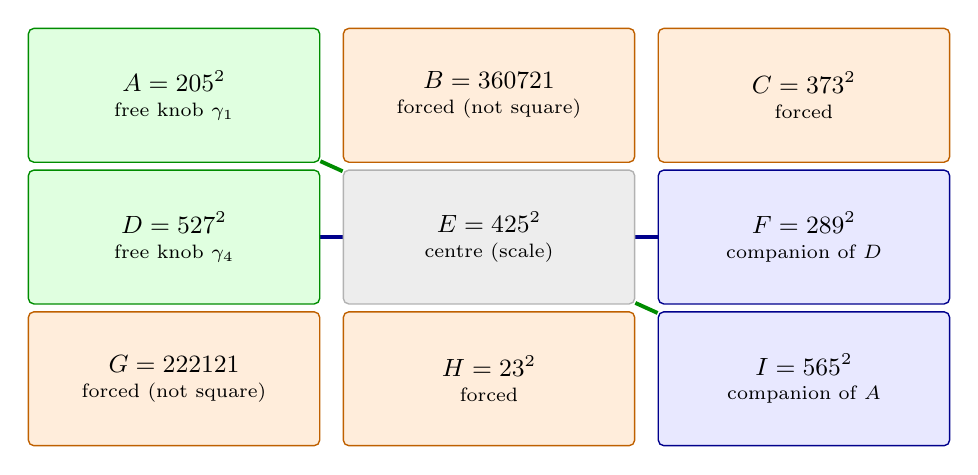
\begin{tikzpicture}[
  cell/.style={draw, minimum width=37mm, minimum height=17mm, align=center,
               line width=0.5pt, rounded corners=2pt, font=\small},
  free/.style={cell, fill=green!12,  draw=green!55!black},
  cent/.style={cell, fill=gray!14,   draw=gray!60},
  comp/.style={cell, fill=blue!9,    draw=blue!55!black},
  forc/.style={cell, fill=orange!14, draw=orange!75!black},
]
\node[free] (A) at (0,3.6)   {$A=205^{2}$\\[-2pt]\scriptsize free knob $\gamma_1$};
\node[forc] (B) at (4,3.6)   {$B=360721$\\[-2pt]\scriptsize forced (not square)};
\node[forc] (C) at (8,3.6)   {$C=373^{2}$\\[-2pt]\scriptsize forced};
\node[free] (D) at (0,1.8)   {$D=527^{2}$\\[-2pt]\scriptsize free knob $\gamma_4$};
\node[cent] (E) at (4,1.8)   {$E=425^{2}$\\[-2pt]\scriptsize centre (scale)};
\node[comp] (F) at (8,1.8)   {$F=289^{2}$\\[-2pt]\scriptsize companion of $D$};
\node[forc] (G) at (0,0)     {$G=222121$\\[-2pt]\scriptsize forced (not square)};
\node[forc] (H) at (4,0)     {$H=23^{2}$\\[-2pt]\scriptsize forced};
\node[comp] (I) at (8,0)     {$I=565^{2}$\\[-2pt]\scriptsize companion of $A$};
\begin{scope}[on background layer]
  \draw[green!55!black, line width=1.4pt] (A) -- (E) -- (I);
  \draw[blue!55!black,  line width=1.4pt] (D) -- (E) -- (F);
\end{scope}
\end{tikzpicture}
\caption{The two knobs and the six dependent cells at $k=425$. The two green cells
$A,D$ are the free choices (a $2$-parameter family in any of the three coordinate
systems); the centre $E=k^{2}$ is a scale. Choosing $A,D$ forces the two blue
companions $I=2k^{2}-A$, $F=2k^{2}-D$ and then the four orange cells
$C=A{+}D{-}k^{2}$, $G=3k^{2}{-}A{-}D$, $B=4k^{2}{-}2A{-}D$, $H=2A{+}D{-}2k^{2}$. All
eight line-sums are $3k^{2}$ automatically; the six coloured non-centre cells each
carry an independent squareness condition. Here four are met ($I,F,C,H$) and two are
not ($G,B$) --- the dependent cells that receive no remaining freedom.}
\label{fig:sixcond}
\end{figure}

\section{The elliptic curve: forced cells as a group law}\label{sec:elliptic}

Theorem~\ref{thm:synthesis} recast the problem as four right triangles on one
circle $s^{2}+d^{2}=k^{2}$ whose areas close, $A_3=A_1+A_2$, $A_4=A_1-A_2$, and
Theorem~\ref{thm:intclosure} as the additive closure of the leg-products
$\delta_i=2s_id_i$. Additive closure of areas of triangles inscribed in a fixed
circle is precisely the arithmetic of an elliptic curve --- the classical theory
of congrua. This section makes the dictionary explicit and exhibits the forced
cells of Section~\ref{sec:dof} as \emph{group-law images}: the two knobs are two
points on the curve, and the forced cells are the points the chord-and-tangent
law delivers from them.

\subsection{Spokes are points; the two knobs are two points}

\begin{definition}[Square-point]\label{def:sqpt}
Let $E$ be the elliptic curve associated (Remark after Theorem~\ref{thm:synthesis})
to area-closure on the circle $s^{2}+d^{2}=k^{2}$. A \emph{square-point} is a
rational point of $E$ corresponding to a spoke of the square: a three-term
arithmetic progression $a^{2},k^{2},b^{2}$ through the centre, equivalently a
lattice point $(s,d)$ with $a=d-s$, $b=d+s$ and offset $\delta=2sd$.
\end{definition}

\begin{proposition}[The additive closure is the group law]\label{prop:grouplaw}
Under the dictionary of Definition~\ref{def:sqpt}, the two free spokes
$\gamma_1,\gamma_2$ --- the two knobs of Theorem~\ref{thm:sixcond} --- are two
rational points $P,Q\in E$, and the two forced spokes are their group-law
combinations,
\[
  \gamma_3=\gamma_1+\gamma_2\ \longleftrightarrow\ P\oplus Q,
  \qquad
  \gamma_4=\gamma_1-\gamma_2\ \longleftrightarrow\ P\ominus Q.
\]
Thus the shift-dependency of Section~\ref{sec:dof} \emph{is} addition on $E$: once
$P$ and $Q$ are chosen the forced points carry no freedom, exactly as the forced
cells $C,G,B,H$ carry none.
\end{proposition}

\subsection{The forced cells are chord-and-reflect images}

On a Weierstrass model $y^{2}=x^{3}+ax+b$ the group law is geometric: the line
through $P$ and $Q$ meets the cubic in exactly one further point (a line meets a
cubic in three), and reflecting that point across the $x$-axis gives
$P\oplus Q$. Because the curve is degree three, this third intersection always
exists and is again rational --- the mechanism a conic (a parabola, degree two,
two intersections) does not possess. The forced spoke, hence the forced cells, is
this manufactured point: not chosen, but produced by $P$ and $Q$.

\begin{figure}[htbp]
\centering
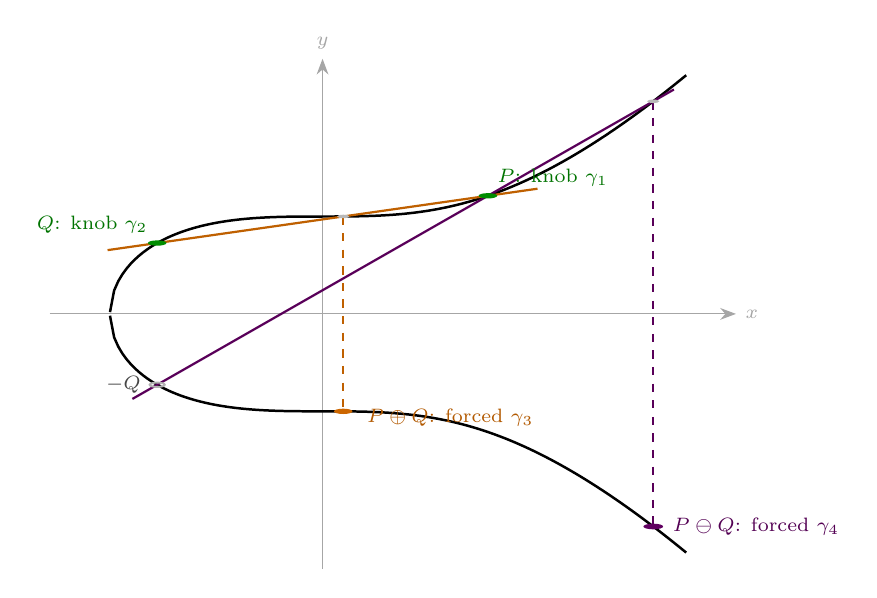
\begin{tikzpicture}[yscale=0.30, xscale=1.05, >={Stealth[length=2mm]}]
  \draw[->, gray!70] (-3.3,0) -- (5.0,0) node[right, font=\scriptsize]{$x$};
  \draw[->, gray!70] (0,-10.8) -- (0,10.8) node[above, font=\scriptsize]{$y$};
  \draw[line width=0.9pt, domain=-2.571:4.4, samples=140, variable=\x]
        plot ({\x},{sqrt(\x*\x*\x+17)});
  \draw[line width=0.9pt, domain=-2.571:4.4, samples=140, variable=\x]
        plot ({\x},{-sqrt(\x*\x*\x+17)});
  \draw[orange!75!black, line width=0.8pt] (-2.6,2.7) -- (2.6,5.3);
  \draw[orange!75!black, dashed, line width=0.7pt] (0.25,4.125) -- (0.25,-4.125);
  \draw[violet!70!black, line width=0.8pt] (-2.3,-3.6) -- (4.25,9.5);
  \draw[violet!70!black, dashed, line width=0.7pt] (4,9) -- (4,-9);
  \fill[green!55!black] (2,5) circle (3.2pt);
  \fill[green!55!black] (-2,3) circle (3.2pt);
  \draw[gray!60, line width=0.7pt] (-2,-3) circle (2.6pt);
  \fill[gray!55] (0.25,4.125) circle (2.1pt);
  \fill[gray!55] (4,9) circle (2.1pt);
  \fill[orange!80!black] (0.25,-4.125) circle (3.2pt);
  \fill[violet!75!black] (4,-9) circle (3.4pt);
  \node[font=\scriptsize, above right, green!45!black] at (2,5)   {$P$: knob $\gamma_1$};
  \node[font=\scriptsize, above left,  green!45!black] at (-2,3)  {$Q$: knob $\gamma_2$};
  \node[font=\scriptsize, left,  gray!55!black]        at (-2.08,-3) {$-Q$};
  \node[font=\scriptsize, right, orange!70!black]      at (0.42,-4.4) {$P\oplus Q$: forced $\gamma_3$};
  \node[font=\scriptsize, right, violet!65!black]      at (4.12,-9) {$P\ominus Q$: forced $\gamma_4$};
\end{tikzpicture}
\caption{Both forced cells as group-law images on the associated elliptic curve
(illustrative model $y^{2}=x^{3}+17$). The two green points $P,Q$ are the free
spokes --- the knobs $\gamma_1,\gamma_2$. The orange line through $P$ and $Q$
meets the cubic at a third point; reflecting it gives $P\oplus Q$, the forced
spoke $\gamma_3=\gamma_1+\gamma_2$ (cells $B,H$). The violet line through $P$ and
$-Q$ (the reflection of $Q$) gives $P\ominus Q$, the forced spoke
$\gamma_4=\gamma_1-\gamma_2$ (cells $C,G$). Both forced spokes are manufactured by
the group law from the two knobs; neither carries any freedom. A nine-square
magic square needs both $P\oplus Q$ and $P\ominus Q$ to be square-points at once.}
\label{fig:ecgrouplaw}
\end{figure}

\begin{remark}[Sum and difference are a matched pair]\label{rem:paralaw}
The two forced points are not independent. Their $x$-coordinates are the two roots
of a single quadratic symmetric in $P,Q$ (the sum/difference addition formulas), and
their canonical heights obey the parallelogram law
\[
  \hat h(P\oplus Q)+\hat h(P\ominus Q)=2\hat h(P)+2\hat h(Q).
\]
So $P\oplus Q$ and $P\ominus Q$ always arrive matched --- making one small forces
the other large. This mirrors the shift arithmetic
$\gamma_3+\gamma_4=2\gamma_1$, $\gamma_3-\gamma_4=2\gamma_2$: sum and difference
balanced around the knobs, exactly as each cell pair balances $2k^{2}$ around the
centre.
\end{remark}

\noindent Where the manufactured point lands is set not by the operation but by the
two knobs. Figure~\ref{fig:ecminus} isolates the subtraction
$P\ominus Q=P\oplus(-Q)$ for a choice with $Q$ on the lower branch: the chord
through $P$ and $-Q$ is nearly flat, so $P\ominus Q$ falls \emph{between} the two
square-points, in contrast to Figure~\ref{fig:ecgrouplaw}, where the same operation
threw the forced point far outside.

\begin{figure}[htbp]
\centering
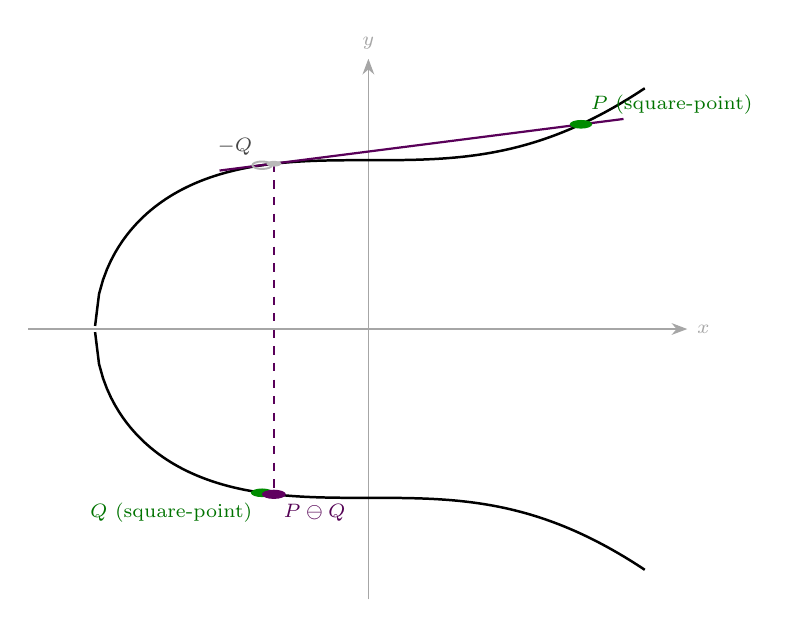
\begin{tikzpicture}[yscale=0.52, xscale=1.35, >={Stealth[length=2mm]}]
  \draw[->, gray!70] (-3.2,0) -- (3.0,0) node[right, font=\scriptsize]{$x$};
  \draw[->, gray!70] (0,-6.6) -- (0,6.6) node[above, font=\scriptsize]{$y$};
  \draw[line width=0.9pt, domain=-2.571:2.6, samples=140, variable=\x]
        plot ({\x},{sqrt(\x*\x*\x+17)});
  \draw[line width=0.9pt, domain=-2.571:2.6, samples=140, variable=\x]
        plot ({\x},{-sqrt(\x*\x*\x+17)});
  \draw[violet!70!black, line width=0.8pt] (-1.4,3.87) -- (2.4,5.13);
  \draw[violet!70!black, dashed, line width=0.7pt] (-0.889,4.037) -- (-0.889,-4.037);
  \fill[green!55!black] (2,5) circle (3pt);
  \fill[green!55!black] (-1,-4) circle (3pt);
  \draw[gray!60, line width=0.7pt] (-1,4) circle (2.6pt);
  \fill[gray!55] (-0.889,4.037) circle (2pt);
  \fill[violet!75!black] (-0.889,-4.037) circle (3.2pt);
  \node[font=\scriptsize, above right, green!45!black] at (2,5)   {$P$ (square-point)};
  \node[font=\scriptsize, below left,  green!45!black] at (-1,-4) {$Q$ (square-point)};
  \node[font=\scriptsize, above left,  gray!55!black]  at (-1,4)  {$-Q$};
  \node[font=\scriptsize, below right, violet!65!black] at (-0.889,-4.037) {$P\ominus Q$};
\end{tikzpicture}
\caption{The subtraction view, $P\ominus Q=P\oplus(-Q)$. The second square-point
$Q$ is taken on the lower branch, so its reflection $-Q$ is nearly level with $P$
and the chord $P\,\text{--}\,(-Q)$ is almost flat; its third intersection sits near
the axis and reflecting gives $P\ominus Q=(-\tfrac89,-\tfrac{109}{27})$, lying
\emph{between} the two square-points $P$ and $Q$. The operation is the same group
law as in Figure~\ref{fig:ecgrouplaw}; only the height budget of
Remark~\ref{rem:paralaw} decides whether the difference lands near the knobs or far
beyond them.}
\label{fig:ecminus}
\end{figure}

\begin{remark}[Negating a knob reflects the outputs]\label{rem:negate}
Replacing $P$ by $-P$ gives
\[
  (-P)\oplus Q=-(P\ominus Q),\qquad (-P)\ominus Q=-(P\oplus Q):
\]
both outputs reflect across the $x$-axis and the sum swaps with the difference. On
the square this is only the freedom to read each spoke from either end,
$k^{2}\mp\gamma$; negating a knob is the same square in mirrored labelling.
\end{remark}

\noindent Figure~\ref{fig:ecnegP} shows both operations from the reflected knob
$-P$ at once: the two chords through $-P$ produce $(-P)\oplus Q$ and
$(-P)\ominus Q$, the mirror images of the sum and difference of
Figure~\ref{fig:ecgrouplaw}.

\begin{figure}[htbp]
\centering
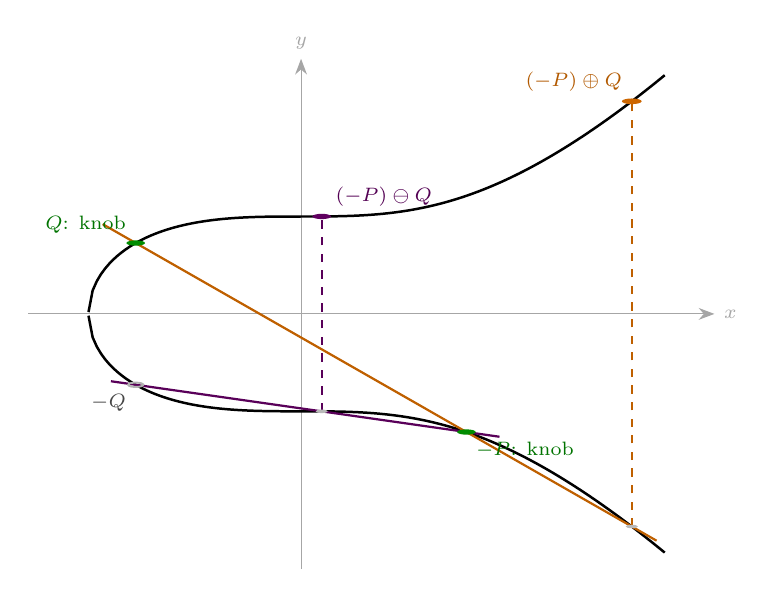
\begin{tikzpicture}[yscale=0.30, xscale=1.05, >={Stealth[length=2mm]}]
  \draw[->, gray!70] (-3.3,0) -- (5.0,0) node[right, font=\scriptsize]{$x$};
  \draw[->, gray!70] (0,-10.8) -- (0,10.8) node[above, font=\scriptsize]{$y$};
  \draw[line width=0.9pt, domain=-2.571:4.4, samples=140, variable=\x]
        plot ({\x},{sqrt(\x*\x*\x+17)});
  \draw[line width=0.9pt, domain=-2.571:4.4, samples=140, variable=\x]
        plot ({\x},{-sqrt(\x*\x*\x+17)});
  \draw[orange!75!black, line width=0.8pt] (-2.4,3.8) -- (4.3,-9.6);
  \draw[orange!75!black, dashed, line width=0.7pt] (4,-9) -- (4,9);
  \draw[violet!70!black, line width=0.8pt] (-2.3,-2.85) -- (2.4,-5.2);
  \draw[violet!70!black, dashed, line width=0.7pt] (0.25,-4.125) -- (0.25,4.125);
  \fill[green!55!black] (2,-5) circle (3.2pt);
  \fill[green!55!black] (-2,3) circle (3.2pt);
  \draw[gray!60, line width=0.7pt] (-2,-3) circle (2.6pt);
  \fill[gray!55] (4,-9) circle (2.1pt);
  \fill[gray!55] (0.25,-4.125) circle (2.1pt);
  \fill[orange!80!black] (4,9) circle (3.4pt);
  \fill[violet!75!black] (0.25,4.125) circle (3.2pt);
  \node[font=\scriptsize, below right, green!45!black] at (2,-5)  {$-P$: knob};
  \node[font=\scriptsize, above left,  green!45!black] at (-2,3)  {$Q$: knob};
  \node[font=\scriptsize, below left,  gray!55!black]   at (-2,-3) {$-Q$};
  \node[font=\scriptsize, above left,  orange!70!black] at (4,9)   {$(-P)\oplus Q$};
  \node[font=\scriptsize, above right, violet!65!black] at (0.3,4.125) {$(-P)\ominus Q$};
\end{tikzpicture}
\caption{The reflected-knob view. Using $-P$ (the reflection of $P$) with the same
$Q$, the orange chord $(-P)\,\text{--}\,Q$ gives $(-P)\oplus Q=(4,9)$ and the violet
chord $(-P)\,\text{--}\,(-Q)$ gives $(-P)\ominus Q=(\tfrac14,\tfrac{33}{8})$. By
Remark~\ref{rem:negate} these are $-(P\ominus Q)$ and $-(P\oplus Q)$: exactly the
sum and difference of Figure~\ref{fig:ecgrouplaw} reflected across the axis, with
their roles swapped. The same magic square, read from the mirrored ends of its
spokes.}
\label{fig:ecnegP}
\end{figure}

\begin{remark}[Sign $=$ branch $=$ below/above]\label{rem:signbranch}
Because $P\ominus Q=P\oplus(-Q)$, there is only one operation; the free choice is the
\emph{sign} of each point. On the curve $P$ and $-P$ are the two branches (same $x$,
opposite $y$); on the square a spoke's two cells are $k^{2}\mp\gamma$ (same gap, one
below and one above the centre). These are the same choice: the sign of a point is the
below/above side of its cell. A \emph{square-point} --- a cell that is a genuine
perfect square --- may sit on the below branch, the above branch, or both, so searching
only one sign (only below roots, or only above roots) can miss a square living on the
other. At $k=425$ every spoke carries its square below and two also above:
\[
\begin{array}{r|cc|c}
\gamma & k^{2}-\gamma & k^{2}+\gamma & \text{square on}\\\hline
138600 & 205^{2} & 565^{2} & \text{both}\\
 97104 & 289^{2} & 527^{2} & \text{both}\\
 41496 & 373^{2} & 222121 & \text{below only}\\
180096 &  23^{2} & 360721 & \text{below only}
\end{array}
\]
so a below-only search sees all four square-points while an above-only search sees only
the two both-square spokes; both nonetheless describe the same square. In general,
though, a required square-point can exist on one branch alone, so both signs must be
searched: the branch of the point, not the choice of $\oplus$ or $\ominus$, is what
locates the square. Geometrically this is the curve's reflection symmetry in the
$x$-axis, $y\mapsto-y$: the graph has two legs meeting at the real root, the two legs
are the two signs (below and above the centre), and a square-point may lie on either
leg --- so one must search both legs of the curve, never only one.
\end{remark}

\begin{remark}[The centre is the fixed point of the reflection]\label{rem:centrefixed}
The same reflection also pins the centre. The map $(x,y)\mapsto(x,-y)$ --- negation
$P\mapsto -P$ --- has fixed locus $y=0$, the axis of symmetry, where the offset
$\delta=2sd$ vanishes. Under the dictionary $\delta=0$ is the degenerate spoke
$\gamma=0$: the centre cell $k^{2}$ itself, the one cell equal to its own companion
$k^{2}\mp0$. Equivalently, in the normalised value view
(Proposition~\ref{prop:scale}) every cell is $1\pm\gamma/k^{2}$ and the antipodal
pairing becomes the reflection $x\mapsto 2-x$, whose unique fixed point is the centre
$1$. Hence $k^{2}$ is not a free parameter but the \emph{fixed point} of the
reflection --- the mean of the eight border cells
(Proposition~\ref{prop:sumfree}), normalised to $1$ and then scaled away entirely.
The two legs of the curve carry the $\pm$ spokes; the axis between them carries the
centre, pinned rather than chosen.
\end{remark}

\begin{figure}[htbp]
\centering
\begin{tikzpicture}[yscale=0.30, xscale=1.05, >={Stealth[length=2mm]}]
  \draw[->, gray!70] (-3.3,0) -- (5.0,0)
        node[right, font=\scriptsize]{$x$ (axis of reflection)};
  \draw[->, gray!70] (0,-10) -- (0,10) node[above, font=\scriptsize]{$y$};
  \draw[line width=0.9pt, domain=-2.571:4.4, samples=140, variable=\x]
        plot ({\x},{sqrt(\x*\x*\x+17)});
  \draw[line width=0.9pt, domain=-2.571:4.4, samples=140, variable=\x]
        plot ({\x},{-sqrt(\x*\x*\x+17)});
  \draw[violet!60!black, dashed, line width=0.7pt] (2,5) -- (2,-5);
  \draw[violet!60!black, dashed, line width=0.7pt] (3.3,7.28) -- (3.3,-7.28);
  \fill[green!55!black] (2,5) circle (2.8pt);
  \fill[green!55!black] (2,-5) circle (2.8pt);
  \fill[green!55!black] (3.3,7.28) circle (2.4pt);
  \fill[green!55!black] (3.3,-7.28) circle (2.4pt);
  \fill[violet!60!black] (2,0) circle (1.5pt);
  \fill[violet!60!black] (3.3,0) circle (1.5pt);
  \fill[orange!85!black] (-2.5713,0) circle (3.6pt);
  \node[font=\scriptsize, right, green!45!black] at (2.05,5)  {$P$};
  \node[font=\scriptsize, right, green!45!black] at (2.05,-5) {$-P$};
  \node[font=\scriptsize, violet!55!black] at (2.7,1.4) {$y\mapsto-y$};
  \node[font=\scriptsize, orange!70!black, right] at (-2.45,1.5)  {centre $\gamma=0$};
  \node[font=\scriptsize, orange!70!black, right] at (-2.45,-1.5) {(fixed point)};
\end{tikzpicture}
\caption{Why $k$ is fixed, not chosen. The curve is symmetric across the $x$-axis,
$(x,y)\mapsto(x,-y)$ (negation $P\mapsto-P$): every point pairs with its mirror on the
other leg (green pairs, dashed connectors), so the two legs carry the $\pm$ spokes
$k^{2}\mp\gamma$. The single point fixed by the reflection is where the curve meets the
axis, $y=0$ --- offset $\delta=0$, the degenerate spoke $\gamma=0$, i.e.\ the centre
$k^{2}$. It lies on the axis of symmetry, pinned rather than chosen; in the normalised
value view it is the fixed point $1$ of $x\mapsto2-x$ (Remark~\ref{rem:centrefixed}).
So $k$ is the reflection's fixed point, not a free parameter.}
\label{fig:centrefixed}
\end{figure}

\begin{remark}[Locating a chord's crossing by symmetry]\label{rem:trig}
Where a chord meets the mirror axis is fixed by the two heights alone. With the axis
as $y=0$, dropping perpendiculars from the endpoints $A=(x_A,y_A)$, $B=(x_B,y_B)$ makes
two similar right triangles sharing the crossing $x_0$ (equal vertical angles), so
\[
  \frac{x_0-x_A}{x_B-x_0}=\frac{|y_A|}{|y_B|},
  \qquad
  x_0=\frac{x_A\,y_B-x_B\,y_A}{y_B-y_A}.
\]
For $A=-P=(2,-5)$, $B=Q=(-2,3)$ this gives $x_0=\frac{6-10}{8}=-\tfrac12$, the run
splitting $1.5:2.5=3:5=|y_A|:|y_B|$. Through the Gaussian dictionary the heights $|y|$
are the offsets $\delta$ of the two spokes, so the crossing is a similar-triangles
average of the two amplitudes --- fixed entirely by the reflection symmetry, though
(unlike the curve's own axis-crossing, the centre $k^{2}$) it is not itself a cell.
\end{remark}

\begin{figure}[htbp]
\centering
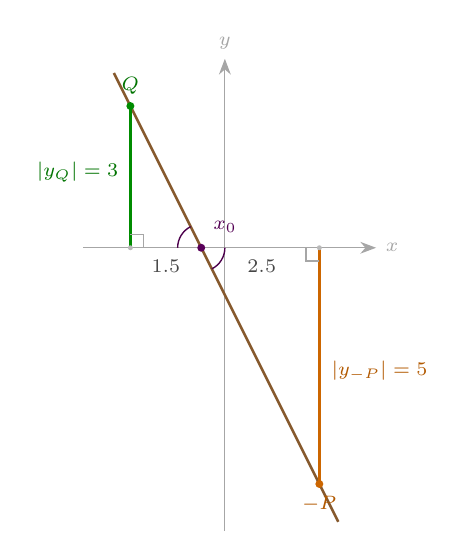
\begin{tikzpicture}[scale=0.6, >={Stealth[length=2mm]}]
  \draw[->,gray!70] (-3,0)--(3.2,0) node[right,font=\scriptsize]{$x$};
  \draw[->,gray!70] (0,-6)--(0,4) node[above,font=\scriptsize]{$y$};
  \draw[brown!70!black, line width=0.9pt] (-2.35,3.7) -- (2.4,-5.8);
  \draw[green!55!black, line width=0.9pt] (-2,3) -- (-2,0);
  \draw[orange!80!black, line width=0.9pt] (2,-5) -- (2,0);
  \draw[gray!70,line width=0.5pt] (-2,0.28)--(-1.72,0.28)--(-1.72,0);
  \draw[gray!70,line width=0.5pt] (2,-0.28)--(1.72,-0.28)--(1.72,0);
  \draw[violet!60!black,line width=0.5pt] ($(-0.5,0)+(180:0.5)$) arc(180:116.57:0.5);
  \draw[violet!60!black,line width=0.5pt] ($(-0.5,0)+(0:0.5)$) arc(0:-63.43:0.5);
  \fill[green!55!black] (-2,3) circle(2.4pt);
  \fill[orange!80!black] (2,-5) circle(2.4pt);
  \fill[violet!70!black] (-0.5,0) circle(2.4pt);
  \fill[gray!55] (-2,0) circle(1.5pt);
  \fill[gray!55] (2,0) circle(1.5pt);
  \node[font=\scriptsize, green!45!black, above]  at (-2,3.05)   {$Q$};
  \node[font=\scriptsize, orange!70!black, below]  at (2,-5.05)   {$-P$};
  \node[font=\scriptsize, green!45!black, left]    at (-2.05,1.6) {$|y_Q|=3$};
  \node[font=\scriptsize, orange!70!black, right]  at (2.05,-2.6) {$|y_{-P}|=5$};
  \node[font=\scriptsize, gray!55!black, below]    at (-1.25,-0.06) {$1.5$};
  \node[font=\scriptsize, gray!55!black, below]    at (0.78,-0.06)  {$2.5$};
  \node[font=\scriptsize, violet!65!black, above right] at (-0.45,0.12) {$x_0$};
\end{tikzpicture}
\caption{Locating the crossing by symmetry. The mirror axis is $y=0$; the heights of the
two endpoints, $|y_Q|=3$ and $|y_{-P}|=5$ (perpendiculars, right angles at their feet),
form two similar right triangles sharing the crossing $x_0$ (equal vertical angles,
marked). The run therefore splits in the ratio of the heights, $1.5:2.5=3:5$, giving
$x_0=(x_A y_B-x_B y_A)/(y_B-y_A)=-\tfrac12$ (Remark~\ref{rem:trig}). The symmetry alone
--- the two amplitudes measured from the axis --- fixes the crossing by trigonometry.}
\label{fig:trigcross}
\end{figure}

\begin{remark}[Crossing versus shift: a lever law]\label{rem:crosslever}
Write each endpoint as a shift from the centre axis: foot (horizontal position) $u_i$
and \emph{signed} shift $\sigma_i=\pm\,2s_id_i$ (positive above the centre, negative
below). The crossing of Remark~\ref{rem:trig} is then a lever balanced by the two
shifts,
\[
  x_0=\frac{u_1\sigma_2-u_2\sigma_1}{\sigma_2-\sigma_1},
  \qquad\text{equivalently}\qquad
  \sigma_2\,(x_0-u_1)=\sigma_1\,(x_0-u_2).
\]
Its position is decided by the \emph{signs} of the shifts, not their sizes: opposite
signs (one spoke above the centre, one below) place $x_0$ \emph{between} the feet;
equal signs place it \emph{outside}. This is once more the below/above rule of
Remark~\ref{rem:signbranch} --- the branch of each spoke governs the crossing --- and
the centre is the degenerate case $\sigma=0$, the fixed axis point $k^{2}$ where the
lever has no moment.
\end{remark}

\begin{figure}[htbp]
\centering
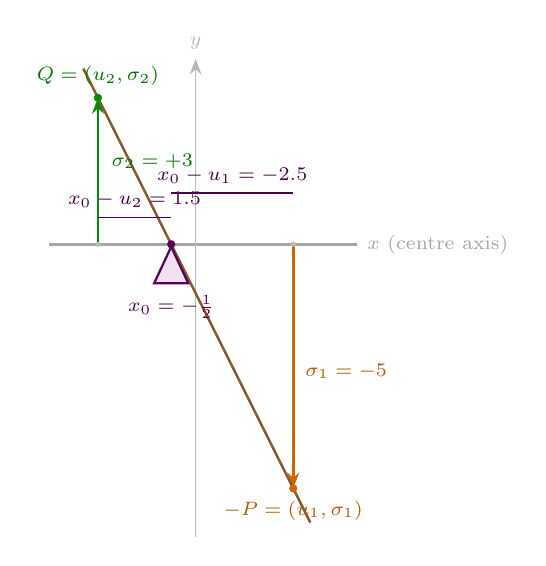
\begin{tikzpicture}[scale=0.62, >={Stealth[length=2mm]}]
  \draw[gray!70, line width=1.1pt] (-3,0)--(3.3,0)
        node[right,font=\scriptsize]{$x$ (centre axis)};
  \draw[->,gray!55] (0,-6)--(0,3.8) node[above,font=\scriptsize]{$y$};
  \draw[green!55!black, line width=1pt, ->] (-2,0)--(-2,3);
  \draw[orange!80!black, line width=1pt, ->] (2,0)--(2,-5);
  \draw[brown!70!black, line width=0.9pt] (-2.3,3.6)--(2.35,-5.7);
  \draw[violet!55!black, line width=0.5pt] (-2,0.55)--(-0.5,0.55);
  \draw[violet!55!black, line width=0.5pt] (-0.5,1.05)--(2,1.05);
  \fill[gray!55] (-2,0) circle(1.5pt);
  \fill[gray!55] (2,0) circle(1.5pt);
  \fill[green!55!black] (-2,3) circle(2.4pt);
  \fill[orange!80!black] (2,-5) circle(2.4pt);
  \fill[violet!70!black] (-0.5,0) circle(2.4pt);
  \draw[violet!65!black, line width=0.8pt, fill=violet!12]
        (-0.5,-0.05)--(-0.85,-0.8)--(-0.15,-0.8)--cycle;
  \node[font=\scriptsize, green!45!black, above]  at (-2,3.05)   {$Q=(u_2,\sigma_2)$};
  \node[font=\scriptsize, orange!70!black, below] at (2,-5.05)   {$-P=(u_1,\sigma_1)$};
  \node[font=\scriptsize, green!45!black, right]  at (-1.92,1.7) {$\sigma_2=+3$};
  \node[font=\scriptsize, orange!70!black, right] at (2.05,-2.6) {$\sigma_1=-5$};
  \node[font=\scriptsize, violet!55!black, above] at (-1.25,0.55){$x_0-u_2=1.5$};
  \node[font=\scriptsize, violet!55!black, above] at (0.75,1.05) {$x_0-u_1=-2.5$};
  \node[font=\scriptsize, violet!65!black, below] at (-0.5,-0.85){$x_0=-\tfrac12$};
\end{tikzpicture}
\caption{The lever law of Remark~\ref{rem:crosslever}. The centre axis is the beam; the
signed shifts $\sigma_2=+3$ (above, at foot $u_2=-2$) and $\sigma_1=-5$ (below, at
$u_1=2$) act as opposing moments, and the chord through the two tips crosses the axis at
the balance point $x_0=-\tfrac12$. There $\sigma_2(x_0-u_1)=\sigma_1(x_0-u_2)$, i.e.\
$3(-2.5)=(-5)(1.5)=-7.5$. Opposite signs put the fulcrum \emph{between} the feet; the
centre $k^{2}$ is the zero-moment point $\sigma=0$.}
\label{fig:lever}
\end{figure}

\begin{remark}[Two axis-anchors replace the second knob]\label{rem:axisanchors}
Two points $\{P,Q\}$ determine the curve $y^{2}=x^{3}+ax+b$: subtracting the two
membership equations gives
\[
  a=\frac{(y_P^{2}-y_Q^{2})-(x_P^{3}-x_Q^{3})}{x_P-x_Q},\qquad
  b=y_Q^{2}-x_Q^{3}-a\,x_Q .
\]
But the second knob can be traded for two points on the mirror axis,
$\{Q;\,x_0,\,x_1\}$, with no loss. The root $x_1$ (the centre) fixes the \emph{curve}:
it and $Q$ give two \emph{linear} equations in $(a,b)$,
\[
  a\,x_1+b=-x_1^{3},\qquad a\,x_Q+b=y_Q^{2}-x_Q^{3},
\]
returning $(a,b)=(0,17)$ for $Q=(-2,3),\ x_1=-\sqrt[3]{17}$. The crossing $x_0$ then
fixes the \emph{chord}: the line through $Q$ meeting the axis at $x_0$ has slope
$y_Q/(x_Q-x_0)$ and re-meets the curve at $P$. Hence
\[
  \{P,Q\}\ \cong\ \{Q;\ x_0,\ x_1\},\qquad
  x_1\rightsquigarrow\text{curve } (a,b),\quad x_0\rightsquigarrow\text{chord (hence }P).
\]
The two free degrees of freedom may be carried as two points, or as one point and its
two axis-anchors --- the centre $x_1$ and the crossing $x_0$.
\end{remark}

\begin{figure}[htbp]
\centering
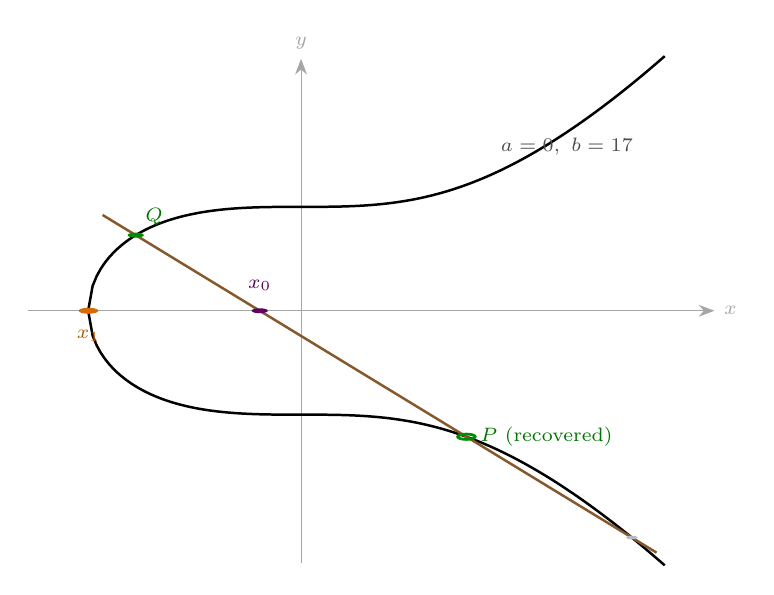
\begin{tikzpicture}[yscale=0.32, xscale=1.05, >={Stealth[length=2mm]}]
  \draw[->, gray!70] (-3.3,0) -- (5.0,0) node[right, font=\scriptsize]{$x$};
  \draw[->, gray!70] (0,-10) -- (0,10) node[above, font=\scriptsize]{$y$};
  \draw[line width=0.9pt, domain=-2.571:4.4, samples=140, variable=\x]
        plot ({\x},{sqrt(\x*\x*\x+17)});
  \draw[line width=0.9pt, domain=-2.571:4.4, samples=140, variable=\x]
        plot ({\x},{-sqrt(\x*\x*\x+17)});
  \draw[brown!70!black, line width=0.9pt] (-2.4,3.8) -- (4.3,-9.6);
  \fill[green!55!black] (-2,3) circle(2.8pt);
  \draw[green!55!black, line width=1pt] (2,-5) circle(3pt);
  \fill[gray!55] (4,-9) circle(2pt);
  \fill[orange!85!black] (-2.571,0) circle(3.4pt);
  \fill[violet!75!black] (-0.5,0) circle(2.8pt);
  \node[font=\scriptsize, green!45!black, above right] at (-2,3)     {$Q$};
  \node[font=\scriptsize, green!45!black, right]       at (2.05,-5)  {$P$ (recovered)};
  \node[font=\scriptsize, orange!70!black, below]      at (-2.571,-0.4) {$x_1$};
  \node[font=\scriptsize, violet!65!black, above]      at (-0.5,0.4) {$x_0$};
  \node[font=\scriptsize, gray!60!black, right]        at (2.3,6.5)  {$a=0,\ b=17$};
\end{tikzpicture}
\caption{Two axis-anchors replace the second knob (Remark~\ref{rem:axisanchors}). From the
one knob $Q=(-2,3)$ and the root $x_1=-\sqrt[3]{17}$ (the curve's axis-crossing, the
centre), two linear equations return the curve $a=0,\ b=17$. The crossing $x_0=-\tfrac12$
then fixes the chord through $Q$ (slope $y_Q/(x_Q-x_0)=-2$), which re-meets the curve at
the recovered point $P=(2,-5)$ (and a third point $(4,-9)$). So $\{Q;x_0,x_1\}$ carries
the same information as $\{P,Q\}$: $x_1$ the curve, $x_0$ the chord.}
\label{fig:axisanchors}
\end{figure}

\subsection{A circular relation: the curve buys no freedom}\label{sec:circular}

The axis-anchor picture must be read with care once the centre is fixed. By
Theorem~\ref{thm:threeparam} a magic square of squares is fixed by $(k,\gamma_1,\gamma_2)$,
of which $k$ is a scale (Proposition~\ref{prop:scale}); the essential freedom is the two
spokes $(\gamma_1,\gamma_2)$. On the host curve the relevant quantities are three points
on the mirror axis: the centre $x_1$ (the root, from $k$), and two that encode the spokes
--- the chord crossing $x_0$ and the abscissa $x_2=x_P$ of the recovered point. They are
\emph{not} independent axes: once the curve is fixed, any two of the spoke-quantities
determine the third, so they close in a loop rather than spread freely.

\begin{proposition}[The spoke quantities satisfy one incidence relation]\label{prop:circular}
Fix the curve (equivalently the centre $x_1=$ root of $x^3+ax+b$). For collinear curve
points $P,Q$ with third intersection $R$, the crossing $x_0$ and the abscissae
$x_2=x_P,\,x_Q$ obey the single relation
\[
  x_0^{2}=\frac{x_P\,x_Q\,x_R+b}{x_P+x_Q+x_R},
  \qquad
  x_R=\Big(\tfrac{y_Q-y_P}{x_Q-x_P}\Big)^{2}-x_P-x_Q .
\]
Hence $\{x_Q,\,x_0,\,x_2\}$ carry one constraint: choosing any two fixes the third. With
$x_1$ the fixed centre and $k$ a scale (Proposition~\ref{prop:scale}), the square keeps
only the two spoke freedoms $(\gamma_1,\gamma_2)$, linked in a closed loop rather than on
independent axes.
\end{proposition}

\noindent So $x_2$ is fixed once $x_0$, the knob $Q$, and the curve $x_1$ are fixed
(for our data $x_0=-\tfrac12,\,b=17$ give $x_0^{2}=\tfrac{(-16)+17}{4}=\tfrac14$,
returning $x_2=2$). The elliptic curve, degree three in $x$, supplies the incidence --- a
line meets it in three points --- but grants \emph{no} new degree of freedom: degree
three is what closes the loop, not what opens it. So passing to the elliptic curve buys
nothing --- the square is still \emph{two} degrees of freedom, the two spokes
$(\gamma_1,\gamma_2)$, on the curve exactly as off it, closed in the circular relation of
Figure~\ref{fig:circular}.

\begin{figure}[htbp]
\centering
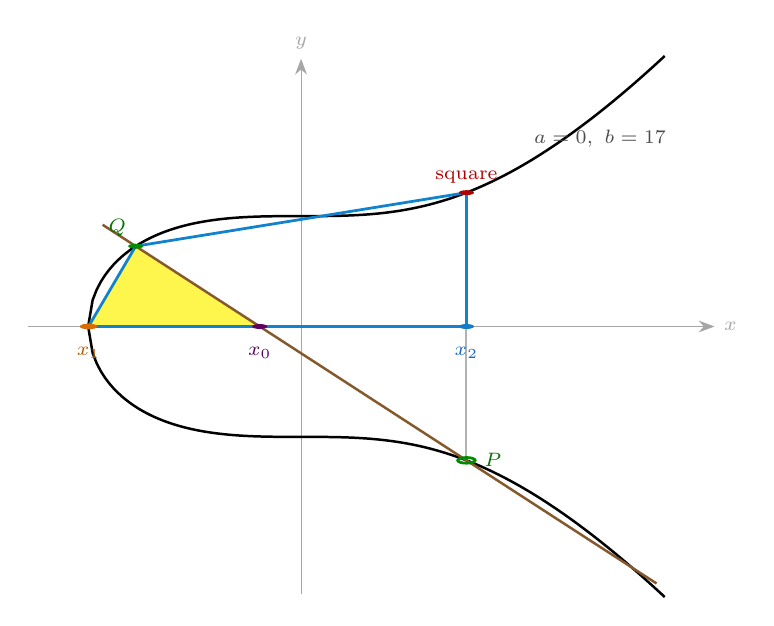
\begin{tikzpicture}[yscale=0.34, xscale=1.05, >={Stealth[length=2mm]}]
  \fill[yellow!70] (-2.571,0)--(-0.5,0)--(-2,3)--cycle;
  \draw[->, gray!70] (-3.3,0) -- (5.0,0) node[right, font=\scriptsize]{$x$};
  \draw[->, gray!70] (0,-10) -- (0,10) node[above, font=\scriptsize]{$y$};
  \draw[line width=0.9pt, domain=-2.571:4.4, samples=140, variable=\x]
        plot ({\x},{sqrt(\x*\x*\x+17)});
  \draw[line width=0.9pt, domain=-2.571:4.4, samples=140, variable=\x]
        plot ({\x},{-sqrt(\x*\x*\x+17)});
  \draw[gray!60, line width=0.7pt] (2,5)--(2,-5);
  \draw[brown!70!black, line width=0.9pt] (-2.4,3.8) -- (4.3,-9.6);
  \draw[cyan!65!blue, line width=1pt] (-2.571,0)--(-2,3)--(2,5)--(2,0)--(-0.5,0)--cycle;
  \fill[orange!85!black] (-2.571,0) circle(3pt);
  \fill[violet!75!black] (-0.5,0) circle(2.6pt);
  \fill[cyan!60!blue] (2,0) circle(2.6pt);
  \fill[green!55!black] (-2,3) circle(2.6pt);
  \fill[red!70!black] (2,5) circle(2.6pt);
  \draw[green!55!black,line width=1pt] (2,-5) circle(3pt);
  \node[font=\scriptsize, orange!70!black, below]  at (-2.571,-0.4){$x_1$};
  \node[font=\scriptsize, violet!65!black, below]  at (-0.5,-0.4)  {$x_0$};
  \node[font=\scriptsize, cyan!45!blue, below]     at (2,-0.4)     {$x_2$};
  \node[font=\scriptsize, green!45!black, above left] at (-2,3)    {$Q$};
  \node[font=\scriptsize, red!70!black, above]      at (2,5)       {square};
  \node[font=\scriptsize, green!45!black, right]    at (2.1,-5)    {$P$};
  \node[font=\scriptsize, gray!60!black, right]     at (2.7,7)     {$a=0,\ b=17$};
\end{tikzpicture}
\caption{The circular relation (Proposition~\ref{prop:circular}). The three axis
quantities $x_1$ (centre), $x_0$ (crossing), $x_2$ (recovered abscissa), together with
the knob $Q$ and the reflected ``square'' point $+P$, close into one loop (blue): fixing
the curve $x_1$ and any two of $\{Q,x_0,x_2\}$ forces the rest. The yellow triangle
$x_1x_0Q$ is one face of it. The degree-three curve provides the incidence but no extra
freedom: the square stays two degrees of freedom (the two spokes), the curve buying
nothing.}
\label{fig:circular}
\end{figure}

\subsection{Why seven and not nine}

\begin{theorem}[Existence is a rank question, not a freedom count]\label{thm:rankopen}
A $3\times3$ magic square of nine squares at centre $k^{2}$ exists iff, for some
two square-points $P,Q\in E$, both $P\oplus Q$ and $P\ominus Q$ are again
square-points (integer legs on the same circle). The two knobs place $P,Q$ freely;
the group law then determines $P\oplus Q,\,P\ominus Q$ with no freedom left, so the
question is whether $E$ \emph{carries} square-points at those two forced positions
--- a property of the rational points of $E$ (its Mordell--Weil rank), not of the
number of parameters.
\end{theorem}

\noindent This is the precise sense in which the two-parameter count of
Section~\ref{sec:dof} does not settle the problem: after the group law consumes the
freedom, existence passes to the arithmetic of $E$. For $k=425$ the chosen $P,Q$
make one of the two forced combinations a square-point (the both-square spoke
$97104$, cells $289^{2},527^{2}$) while the other is not ($\gamma_3=180096$ gives
$23^{2}$ and the non-square $360721$): four of the six dependent cells square, the
seven-square record of Theorem~\ref{thm:target}. A nine-square magic square is a
single centre whose curve carries square-points at \emph{both} forced positions
at once; none has been found, and by the boundary obstruction
(Theorem~\ref{thm:synthesis}, the forbidden apex $s=d$ at the irrational radius
$k=s\sqrt2$) the forced points are pushed toward a place the lattice does not reach.

\begin{remark}[Rank enlarges the supply, not the freedom]\label{rem:rankdof}
Rank and degrees of freedom are different quantities, and it is worth stating that they
do not trade against one another. The Mordell--Weil rank counts the independent rational
points of $E$ --- the \emph{supply} of square-point candidates; a higher rank means more
points from which to draw $P,Q$ and better odds that $P\oplus Q$ and $P\ominus Q$ fall on
square-points. But the square is still placed by exactly two choices, $P$ and $Q$, after
which the group law fixes $P\oplus Q,\,P\ominus Q$ with nothing left to adjust
(Section~\ref{sec:circular}). Hence even on a curve of large rank the problem remains
\emph{two} degrees of freedom: rank changes how \emph{likely} the two forced points are
to be square, never how \emph{many} free points there are. The wall is not a shortage of
freedom but the simultaneous squareness of two forced combinations of two free ones ---
and no amount of rank turns the two knobs into three. This is why the two-parameter count
of Section~\ref{sec:dof} and the arithmetic (rank) of Theorem~\ref{thm:rankopen} are
consistent, not competing: the geometry fixes the freedom at two, the arithmetic decides
whether those two can be met, and passing to the elliptic curve --- of whatever rank ---
buys extra candidates but never an extra knob.

Moreover the two are coupled by the circular relation of Section~\ref{sec:circular}, and
this is what \emph{caps} the value of the extra candidates. A high rank supplies more
rational points, but they help only if the forced images $P\oplus Q,\,P\ominus Q$ ---
already determined by the two free points --- happen to fall on them, \emph{closing} the
loop. One cannot place the forced points on the new candidates independently; they must
close at the end. So a large rank raises the density of possible landing sites without
loosening the closure that binds them to the two choices: more candidates, each still
obliged to close the same two-freedom loop. The geometry (closure) and the arithmetic
(supply) do not add --- they multiply against each other, and the circular relation is
their meeting point: every candidate the rank offers must still return through the loop,
so the abundance is spent on \emph{odds}, never on \emph{room}.

And the odds themselves lie \emph{inside} the two degrees of freedom, never beyond them:
every candidate the rank supplies is reached by the same two free choices, so meeting the
six squareness conditions of Theorem~\ref{thm:sixcond} stays six constraints on a
two-dimensional family --- overdetermined by four --- at every rank. Rank changes only how
densely that two-dimensional family is populated by rational points, never its dimension.
Six conditions to be fitted into two degrees of freedom is therefore the invariant wall:
the whole problem is to place six square-demands inside a two-parameter family, and no
arithmetic abundance, of any rank, enlarges the two or lowers the six.
\end{remark}

\begin{remark}[The six conditions are coupled, not independent]\label{rem:coupled}
``Six conditions in two degrees of freedom'' must not be read as six independent events.
The two free choices are $A,D$ (taken square); the six conditions then fall on the
\emph{dependent} cells, each an integer-linear form in $(k^2,A,D)$,
\[
  I=2k^2-A,\quad F=2k^2-D,\quad C=A+D-k^2,\quad G=3k^2-A-D,\quad
  B=4k^2-2A-D,\quad H=2A+D-2k^2
\]
(Theorem~\ref{thm:sixcond}). These six have Jacobian rank \emph{two} in $(A,D)$: only $I$
depends on $A$ alone and only $F$ on $D$ alone, while $C,G,B,H$ depend on both. Hence no
three of them are independent of the other three --- any triple that involves both knobs
already fixes $(A,D)$ and therefore the rest, and the relations $I+F+C=3k^2$, $C+G=2k^2$,
$B+H=2k^2$ cross every partition. None of the six can be tuned on its own --- all are locked the
instant $A,D$ are chosen --- so they are not six separate chances but one rigid system
driven by two knobs. Hence they are strongly \emph{coupled}: moving $A,D$ to make one
dependent cell a square shifts the other five as well, and generally pushes some off a
square. There is no product of six probabilities to raise independently; there are two
choices that fix all six values together, which is exactly why success is rarer than a
na\"ive independence estimate would suggest --- and why the record sticks at four of the
six (Theorem~\ref{thm:target}) rather than climbing cell by cell. The circular relation of
Section~\ref{sec:circular} \emph{is} this coupling: the last cells fight the first rather
than add to them, and each square gained costs freedom the remaining ones needed. The six
sit inside a single closed convex, the two triples interlocked rather than independent
(Figure~\ref{fig:nohexagon}); the algebraic form of the same coupling is
Figure~\ref{fig:coupling}.
\end{remark}

\begin{figure}[htbp]
\centering
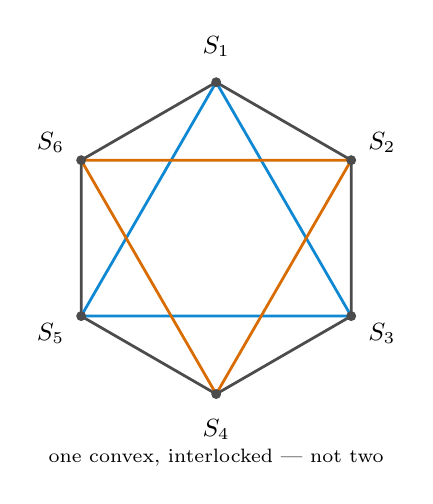
\begin{tikzpicture}[scale=0.9, font=\small]
  \foreach \a/\lab in {90/1,30/2,-30/3,-90/4,210/5,150/6}
    \coordinate (S\lab) at (\a:2.2);
  \draw[black!70, line width=1pt] (S1)--(S2)--(S3)--(S4)--(S5)--(S6)--cycle;
  \draw[cyan!70!blue, line width=1pt] (S1)--(S3)--(S5)--cycle;
  \draw[orange!85!black, line width=1pt] (S2)--(S4)--(S6)--cycle;
  \foreach \a/\lab in {90/1,30/2,-30/3,-90/4,210/5,150/6}{
    \fill[black!70] (\a:2.2) circle(2pt);
    \node at (\a:2.7) {$S_{\lab}$};
  }
  \node[black!65!black, font=\scriptsize] at (0,-3.1) {one convex, interlocked --- not two};
\end{tikzpicture}
\caption{All six lie inside \emph{one} closed convex. The six conditions are the vertices
of a single hexagon; the two inscribed triples $\{S_1,S_3,S_5\}$ (blue) and
$\{S_2,S_4,S_6\}$ (orange) \emph{interlock} and cannot be pulled apart into two independent
convex pieces. This is the coupling made visible: rank two in $(A,D)$
(Remark~\ref{rem:coupled}) means $(S_1,S_2,S_3)$ always depends on $(S_4,S_5,S_6)$, so the
six squareness demands live in a single closure, never split three-and-three into separate
ones. The algebraic form of the same fact --- all six functions of the two knobs $A,D$ ---
is Figure~\ref{fig:coupling}.}
\label{fig:nohexagon}
\end{figure}

\begin{figure}[htbp]
\centering
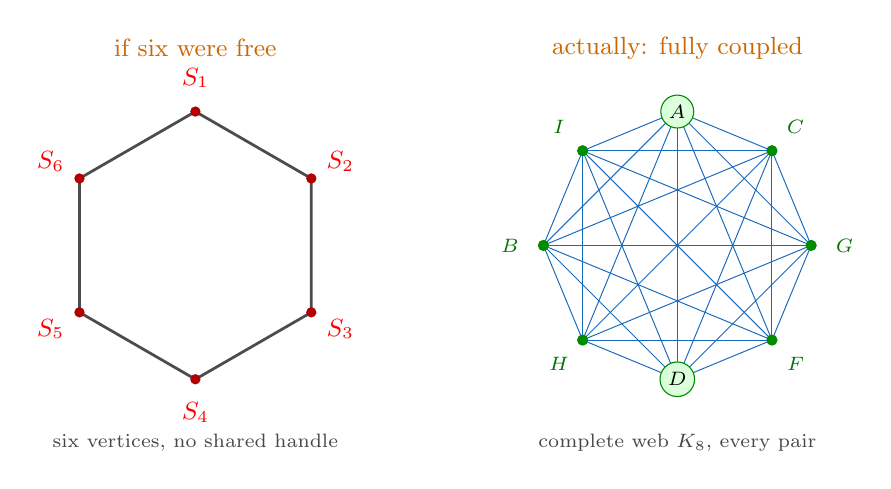
\begin{tikzpicture}[scale=0.85, font=\small]
  \begin{scope}[shift={(0,0)}]
    \foreach \a/\lab in {90/1,30/2,-30/3,-90/4,210/5,150/6}
      \coordinate (L\lab) at (\a:2);
    \draw[black!70, line width=1pt] (L1)--(L2)--(L3)--(L4)--(L5)--(L6)--cycle;
    \foreach \a/\lab in {90/1,30/2,-30/3,-90/4,210/5,150/6}{
      \fill[red!70!black] (\a:2) circle(2.2pt);
      \node[red] at (\a:2.5) {$S_{\lab}$};
    }
    \node[orange!80!black] at (0,2.95) {if six were free};
    \node[gray!55!black, font=\scriptsize] at (0,-2.95) {six vertices, no shared handle};
  \end{scope}
  \begin{scope}[shift={(7.2,0)}]
    \coordinate (A) at (90:2);  \coordinate (C) at (45:2);
    \coordinate (I) at (135:2); \coordinate (B) at (180:2);
    \coordinate (H) at (225:2); \coordinate (D) at (270:2);
    \coordinate (F) at (315:2); \coordinate (G) at (0:2);
    \foreach \u/\v in {A/C,A/I,A/B,A/H,A/D,A/G,A/F,C/I,C/B,C/H,C/D,C/F,C/G,%
                       I/B,I/H,I/F,I/G,I/D,B/H,B/D,B/F,B/G,H/D,H/F,H/G,D/F,D/G,F/G}
      \draw[cyan!45!blue, line width=0.35pt] (\u)--(\v);
    \foreach \n/\ang in {C/45,I/135,B/180,H/225,F/315,G/0}
      \fill[green!55!black] (\ang:2) circle(2.4pt);
    \node[circle,draw=green!55!black,fill=green!14,inner sep=1.5pt] at (90:2)  {\scriptsize$A$};
    \node[circle,draw=green!55!black,fill=green!14,inner sep=1.5pt] at (270:2) {\scriptsize$D$};
    \foreach \n/\ang in {C/45,I/135,B/180,H/225,F/315,G/0}
      \node[green!45!black] at (\ang:2.5) {\scriptsize$\n$};
    \node[orange!80!black] at (0,2.95) {actually: fully coupled};
    \node[gray!55!black, font=\scriptsize] at (0,-2.95) {complete web $K_8$, every pair};
  \end{scope}
\end{tikzpicture}
\caption{The six on one closed hexagon, and the full dependency web. \emph{Left:} were the
six conditions free they would be independent vertices with no shared handle. \emph{Right:}
as a coupled system the eight border cells form the \emph{complete} graph $K_8$: a generic
change of the two knobs $(A,D)$ moves \emph{all eight} cells at once, so every pair
co-varies and every node has degree seven. (Writing $F=2k^2-D$, $I=2k^2-A$ in the $(A,D)$
basis makes $F,I$ look tied to a single knob, but the row and column sums re-adjust every
cell, so $F$ and $I$ move with the rest --- the graph is fully connected, not
near-connected.) One fixes $(A,D)$ and the octagon settles the other cells through its
relations; normalised by $k^2$ the eight vertex-weights sum to $8$ (Proposition~\ref{prop:sumfree}).
This is why no three cells can be freed from the other three (Remark~\ref{rem:coupled}), and
the record settles at four (Theorem~\ref{thm:target}) rather than climbing cell by cell.}
\label{fig:coupling}
\end{figure}

\subsection{A network formulation and a bounded search}\label{sec:network}

Reading the eight border cells as the fully coupled network of Figure~\ref{fig:coupling}
turns the problem into a two-input relaxation. Fix the centre $k$ and inject one square
$A=a^2$; the single free knob $D$ then \emph{settles} every other cell through the
row/column/diagonal sums,
\[
  I=2k^2-A,\ \ F=2k^2-D,\ \ C=A+D-k^2,\ \ G=3k^2-A-D,\ \ B=4k^2-2A-D,\ \ H=2A+D-2k^2,
\]
and one never needs the raw values --- only the normalised weights $w_i=\text{cell}_i/k^2$,
which satisfy $\sum_i w_i=8$ (Proposition~\ref{prop:sumfree}). The scoring function counts
how many weights are rational squares (perfect-square cells), with the nine entries required
\emph{distinct} --- the degenerate solution (three copies each of $205^2,425^2,565^2$) is
excluded.

\begin{lstlisting}[language=Python]
from math import isqrt
def score(k, A, D):
    e = k*k
    cells = [A, 4*e-2*A-D, A+D-e, D, 2*e-D, 3*e-A-D, 2*A+D-2*e, 2*e-A]  # 8 border cells
    if any(v <= 0 for v in cells):   return -1
    if len(set(cells + [e])) != 9:   return -1               # distinct entries required
    return sum(isqrt(v)**2 == v for v in cells)              # how many are squares
\end{lstlisting}

\noindent Sweeping the free knob $D=d^2$ for the input $A=205^2$ at $k=425$ settles at
$D=527^2$ with score $6$ of $8$ (seven of nine), recovering the record. A bounded scan over
all centres and square inputs finds nothing better: for $k\le150$ the maximum is $5$ of $8$
(six of nine), and $425$ is the smallest centre reaching seven of nine; no centre examined,
here or elsewhere, exceeds it. As throughout, this is empirical --- ``none better below the
bound'' --- and not a proof: an eighth or ninth square would require the coupled network to
settle two more forced cells onto squares at once, the simultaneous landing the two-input
coupling makes so rare (Remark~\ref{rem:coupled}).

\medskip\noindent The naive sweep is $O(n^3)$ in the bound (centres times two inputs). The
objective is discrete --- squareness is not differentiable and the solutions are isolated
integer points, so gradient or backpropagation methods do not apply --- but the arithmetic
gives a clean $O(n^2)$ replacement: the companions $I,F$ are square only when $A,D$ lie in a
both-square pair $2k^2=x^2+y^2$, and those members are found in one $O(k)$ pass per centre
and then combined. This reaches $k\le5000$ in a few seconds, where the naive scan struggles
past $k=250$. The ceiling holds throughout: the best is always seven of nine, and the
centres attaining it are exactly the multiples $425m$ --- scale copies of $425$
(Proposition~\ref{prop:scale}), no primitive centre beyond $425$ appearing and nothing above
seven of nine found. Still empirical, still not a proof.

\begin{remark}[The two knobs are a corner and an edge]\label{rem:corneredge}
The two free cells are not interchangeable. In the settlement formulas $A$ carries
coefficient $2$ ($B=4k^2-2A-D$, $H=2A+D-2k^2$) while $D$ carries $1$, so $A$ occupies a
\emph{corner} of the grid and $D$ an \emph{edge}. Consequently, entering the network
(Section~\ref{sec:network}) at a given square value recovers a square's full score only if
that value can sit at the $A$-corner --- i.e.\ only if it is a corner cell of the target
square. For the record at $k=425$ the three square-valued corners each root a $7/9$
settlement, while the three square-valued edges fall short:
\begin{center}\small
\begin{tabular}{lcccccc}
\hline
root     & $205^2$ & $373^2$ & $565^2$ & $527^2$ & $289^2$ & $23^2$\\
position & corner  & corner  & corner  & edge    & edge    & edge\\
best     & $7/9$   & $7/9$   & $7/9$   & $6/9$   & $6/9$   & $4/9$\\
\hline
\end{tabular}
\end{center}
So the swap $A\leftrightarrow D$ is not a symmetry: corner and edge are distinct roles, and
rooting at an edge value drops the score. Crucially, re-rooting does not change the
\emph{algebra} --- $A$ is always the coefficient-$2$ corner and $D$ the coefficient-$1$
edge --- it only changes which \emph{value} is placed at the fixed corner. The root's
influence is therefore \emph{geometric} (a value-to-position assignment), not algebraic: a
value that is a corner cell of the target square fits the corner and keeps the score, while
an edge value forced onto the corner yields a different, lower settlement. A square looks
robust to re-rooting only when, like the record, it carries several square-valued corners.

\medskip\noindent Rooting at the corner is exactly the hypotenuse view of
Section~\ref{sec:selectk}. The corner $A$, the centre $E$, and the opposite corner $I$ form
the diagonal
\[
  A=(d-s)^2,\qquad E=k^2=s^2+d^2,\qquad I=2k^2-A=(d+s)^2,
\]
so the corner--centre--corner triple \emph{is} the Pythagorean triple $(s,d,k)$, and choosing
the corner value chooses its leg pair $s=\tfrac{\sqrt I-\sqrt A}{2}$, $d=\tfrac{\sqrt I+\sqrt A}{2}$
--- the $\tfrac{q-p}{8}\cdot4,\ \tfrac{p+q}{8}\cdot4$ recipe. For $425$, corners $205^2,565^2$
give $s=180,\ d=385$ with $180^2+385^2=425^2$. Only a value that is $(d-s)^2$ for some leg
pair of $k$ --- a genuine hypotenuse cell --- can hold the corner and keep the diagonal
all-square; an edge value belongs to the middle-row spoke (a different triple) and breaks the
diagonal when forced to the corner.
\end{remark}

\begin{figure}[htbp]
\centering
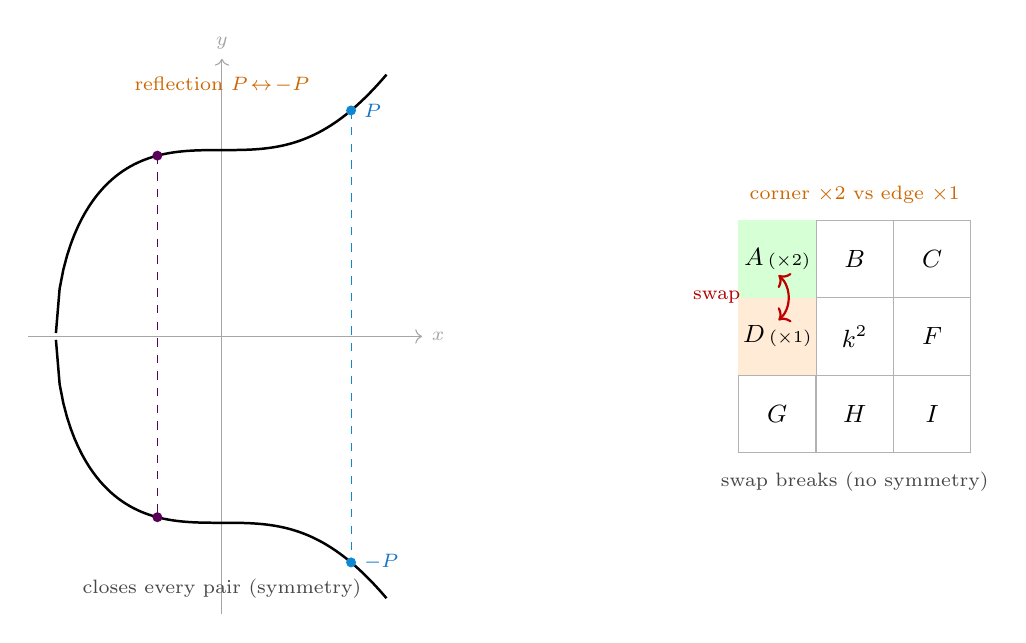
\begin{tikzpicture}[scale=0.82, font=\small]
  \begin{scope}[shift={(0,0)}]
    \draw[->,gray!70] (-3,0)--(3.1,0) node[right,font=\scriptsize]{$x$};
    \draw[->,gray!70] (0,-4.3)--(0,4.3) node[above,font=\scriptsize]{$y$};
    \draw[line width=0.9pt, domain=-2.571:2.55, samples=90, variable=\x]
          plot ({\x},{0.7*sqrt(\x*\x*\x+17)});
    \draw[line width=0.9pt, domain=-2.571:2.55, samples=90, variable=\x]
          plot ({\x},{-0.7*sqrt(\x*\x*\x+17)});
    \draw[cyan!70!blue, dashed] (2,3.5)--(2,-3.5);
    \draw[violet!70!black, dashed] (-1,2.8)--(-1,-2.8);
    \fill[cyan!70!blue] (2,3.5) circle(2.2pt);   \fill[cyan!70!blue] (2,-3.5) circle(2.2pt);
    \fill[violet!70!black] (-1,2.8) circle(2.2pt); \fill[violet!70!black] (-1,-2.8) circle(2.2pt);
    \node[font=\scriptsize,cyan!55!blue,right] at (2.05,3.5) {$P$};
    \node[font=\scriptsize,cyan!55!blue,right] at (2.05,-3.5) {$-P$};
    \node[font=\scriptsize,orange!80!black] at (0,3.9) {reflection $P\!\leftrightarrow\!-P$};
    \node[font=\scriptsize,gray!55!black] at (0,-3.9) {closes every pair (symmetry)};
  \end{scope}
  \begin{scope}[shift={(8,-1.8)}]
    \foreach \i in {0,1,2,3} \draw[gray!60] (\i*1.2,0)--(\i*1.2,3.6);
    \foreach \j in {0,1,2,3} \draw[gray!60] (0,\j*1.2)--(3.6,\j*1.2);
    \fill[green!16] (0,2.4) rectangle (1.2,3.6);
    \fill[orange!16] (0,1.2) rectangle (1.2,2.4);
    \node at (0.6,3.0) {$A\,{\scriptstyle(\times2)}$};
    \node at (1.8,3.0) {$B$}; \node at (3.0,3.0) {$C$};
    \node at (0.6,1.8) {$D\,{\scriptstyle(\times1)}$};
    \node at (1.8,1.8) {$k^2$}; \node at (3.0,1.8) {$F$};
    \node at (0.6,0.6) {$G$}; \node at (1.8,0.6) {$H$}; \node at (3.0,0.6) {$I$};
    \draw[red!75!black, <->, line width=0.8pt] (0.62,2.75) to[bend left=48] (0.62,2.05);
    \node[font=\scriptsize,red!70!black,left] at (0.18,2.4) {swap};
    \node[font=\scriptsize,orange!80!black] at (1.8,4.0) {corner $\times2$ vs edge $\times1$};
    \node[font=\scriptsize,gray!55!black] at (1.8,-0.45) {swap breaks (no symmetry)};
  \end{scope}
\end{tikzpicture}
\caption{Two layers. \emph{Left (on the curve):} the elliptic curve's reflection across the
$x$-axis, $P\leftrightarrow-P$, closes every antipodal pair (cell $+$ companion $=2k^2$) --- a
genuine symmetry that always holds, treating the diagonal pair and the middle-row pair
identically. \emph{Right (in the grid):} the two free cells sit at a corner ($A$, coefficient
$2$) and an edge ($D$, coefficient $1$); swapping them is \emph{not} a symmetry, so an edge
value forced to the corner breaks the score. The closing symmetry lives on the curve; the
breaking asymmetry lives on the grid --- different layers, which is why the swap cannot be
shown ``breaking'' on the curve itself.}
\label{fig:twolayers}
\end{figure}

\noindent One might still hope to see the swap on the curve as ``which point is doubled,''
since the corner $A$ carries coefficient $2$. But that coefficient is
\emph{convention-dependent}, not an intrinsic doubling. The four gaps of the $425$ square,
$\{41496,\,97104,\,138600,\,180096\}$, are written $\{|p|,|q|,|p{+}q|,|2p{+}q|\}$ with a
coefficient $2$ in the corner--edge labelling $(p,q)=(-138600,97104)$, and equally
$\{g_1,g_2,g_1{+}g_2,g_1{-}g_2\}$ --- with \emph{no} doubling --- in the symmetric
two-diagonal labelling $(g_1,g_2)=(138600,41496)$. The same four gaps, one labelling with a
$2$ and one without. So there is no intrinsic doubled point: the corner/edge asymmetry is a
labelling of grid positions, not a group-law doubling on the curve, which is why the honest
picture is the two-layer Figure~\ref{fig:twolayers} and not a single curve diagram.

\begin{remark}[The network closes the symmetry; squareness rides on top]\label{rem:symmarith}
The central symmetry --- opposite cells summing to $2k^2$, every line to $3k^2$ --- is not
something to be arranged but something the $K_8$ network \emph{enforces}: for \emph{any} value
placed at $A$ the coupling settles $I=2k^2-A$ and then, through $D$, all remaining cells,
always preserving the antipodal pairing and the magic sums (Section~\ref{sec:circular}).
Changing $A$ therefore never breaks the symmetry; the network re-closes it across all eight
cells. What $A$ changes is the \emph{arithmetic} layered on top --- how many cells are perfect
squares (the score) and whether $A$ holds a genuine corner/hypotenuse cell
(Remark~\ref{rem:corneredge}). So the $3\times3$ structure separates cleanly into two levels:
a central symmetry the network always closes, and a squareness condition the two free choices
can only partly meet --- the former guaranteed, the latter the open difficulty.
\end{remark}

\subsection{What selects a centre: mod 8, closure, and the hypotenuse}\label{sec:selectk}

Three things are commonly blamed for why $425$ works --- the number of square roots it
offers, its size, and its factor count. None is the operative reason; what a centre must
provide is structural.

\paragraph{Not the number of roots.} A centre may present many square inputs that each
settle to a decent score, yet they do not combine: each is one two-degree-of-freedom
settlement (Section~\ref{sec:circular}), and the favourable cells of different settlements
live in different closures. For $k=442$ five input roots reach six of nine across two
distinct squares, and none can be merged to exceed it. Abundance of roots is not progress.

\paragraph{Requirement 1: primitive mod $8$.} By Theorem~\ref{thm:mod8} and
Corollary~\ref{cor:oddk} a primitive square needs $k$ odd, so every cell is $\equiv1\pmod8$;
an even $k$ merely rescales a smaller one. The quick signature is $k^2/8$: an odd $k$ gives
fractional part $\tfrac18$ (e.g.\ $425^2/8=22578.125$), an even $k$ gives $0$ or $\tfrac12$
(e.g.\ $422^2/8=22260.5$, since $422^2\equiv4$). Only the odd centres are primitive.

\paragraph{Requirement 2: the roots must close.} Beyond mod $8$, the chosen roots must
assemble into the closed two-parameter configuration of Section~\ref{sec:circular} with the
forced cells also square. This closure --- not the supply of roots --- is decisive, and for
the full nine it is the open problem.

\paragraph{Choosing a centre: the hypotenuse rule.} The raw material for closure is the set
of \emph{both-square spokes}, and each is a Pythagorean triple. A pair of cell-roots $(p,q)$
around $k$ has legs
\[
  s=\frac{q-p}{2}\ (\text{half-difference}),\qquad d=\frac{p+q}{2}\ (\text{mean}),
  \qquad s^2+d^2=k^2 ,
\]
so $(s,d,k)$ is a right triangle and $p=d-s,\ q=d+s$. A both-square spoke exists at $k$ iff
$k$ is the \emph{hypotenuse} of an integer right triangle; a centre supplies \emph{many}
spokes iff it is a hypotenuse in many ways --- which happens exactly when $k$ carries primes
$\equiv1\pmod4$.

\paragraph{Why $425=5^2\cdot17$.} Both $5$ and $17$ are $\equiv1\pmod4$, so $425$ is a
hypotenuse seven ways; the seven triples and their both-square pairs are
\begin{center}\small
\begin{tabular}{ccc@{\qquad}ccc}
\hline
$s$ & $d$ & pair $(d\!-\!s,\,d\!+\!s)$ & $s$ & $d$ & pair\\
\hline
$297$ & $304$ & $(7,601)$   & $180$ & $385$ & $(205,565)$\\
$255$ & $340$ & $(85,595)$  & $119$ & $408$ & $(289,527)$\\
$200$ & $375$ & $(175,575)$ & $87$  & $416$ & $(329,503)$\\
$65$  & $420$ & $(355,485)$ &       &       & \\
\hline
\end{tabular}
\end{center}
The pairs $(205,565)$ and $(289,527)$ are the two both-square spokes of the record square.

\medskip\noindent\emph{Worked example (reading the legs off a pair).} Take $(p,q)=(17,25)$.
Dividing by $8$ keeps the mean over the eight border vertices, and multiplying by $4$
restores the four-above/four-below split, so the legs come out as
\[
  \frac{q-p}{8}=\frac{25-17}{8}=1,\qquad 1\cdot4=s=4;
  \qquad\qquad
  \frac{p+q}{8}=\frac{17+25}{8}=5.25,\qquad 5.25\cdot4=d=21 .
\]
Then $s^2+d^2=4^2+21^2=457$, which is \emph{not} a perfect square: $457$ is prime and
$\equiv1\pmod4$ but is not itself a hypotenuse, so $(17,25)$ seeds no spoke. A second pair
$(35,43)$ behaves the same way: $\tfrac{43-35}{8}\cdot4=4=s$ and
$\tfrac{35+43}{8}\cdot4=39=d$, whence $s^2+d^2=4^2+39^2=1537$, again not a perfect square
--- and here $43\equiv3\pmod8$ (equivalently $\equiv3\pmod4$), so the prime $43$ is itself
no hypotenuse. (The same recipe on $(205,565)$ gives $\tfrac{360}{8}\cdot4=180=s$ and
$\tfrac{770}{8}\cdot4=385=d$ with $180^2+385^2=425^2$ --- a valid spoke.)

\medskip\noindent\emph{Failing case (a prime not $\equiv1\bmod4$).} A centre built only from
primes $\equiv3\pmod4$ fails outright. Take $k=21=3\cdot7$: it is odd, so it \emph{passes}
the mod-$8$ test ($21^2/8=55.125$, cells $\equiv1\pmod8$), yet $21^2=441$ is a sum of two
squares only trivially, $441=21^2+0^2$. No leg pair $s,d>0$ solves $s^2+d^2=21^2$, so $21$ is
the hypotenuse of nothing and seeds no both-square spoke --- the search never even starts.
This is the decisive difference from $425$: passing mod $8$ (odd) is necessary but useless
without a prime $\equiv1\pmod4$ to make $k$ a hypotenuse. The intermediate case
$851=23\cdot37$ carries one such prime ($37\equiv1\pmod4$) but only one, so it is a
hypotenuse a single way --- one spoke, too few to close.

\paragraph{How many spokes: count the primes $\equiv1\pmod4$ (not $\pmod8$).} The number of
both-square spokes grows with the distinct primes $\equiv1\pmod4$ dividing $k$ (each raises
it, higher powers raise it more). Crucially it is $\equiv1\pmod4$, not $\equiv1\pmod8$:
\begin{center}\small
\begin{tabular}{rlccrc}
\hline
$k$ & factors & primes $\equiv1\ (4)$ & primes $\equiv1\ (8)$ & spokes & best\\
\hline
$5$    & $5$                & $5$        & ---   & $1$  & $0/9$\\
$25$   & $5^2$              & $5$        & ---   & $2$  & $6/9$\\
$65$   & $5\cdot13$         & $5,13$     & ---   & $4$  & $5/9$\\
$425$  & $5^2\cdot17$       & $5,17$     & $17$  & $7$  & $7/9$\\
$1105$ & $5\cdot13\cdot17$  & $5,13,17$  & $17$  & $13$ & $6/9$\\
$5525$ & $5^2\cdot13\cdot17$& $5,13,17$  & $17$  & $22$ & $7/9$\\
$2009$ & $7^2\cdot41$       & $41$       & $41$  & $1$  & $0/9$\\
\hline
\end{tabular}
\end{center}
The spoke count follows the $\equiv1\pmod4$ column, never the $\equiv1\pmod8$ one: $65$ has
four spokes with \emph{no} prime $\equiv1\pmod8$ (both $5,13\equiv5\pmod8$), while $2009$
carries the prime $41\equiv1\pmod8$ yet has only one spoke. So the productive prime $5$ ---
behind the $3\text{-}4\text{-}5$ triangle --- is $\equiv5\pmod8$, and a mod-$8$ filter would
wrongly discard it. More distinct primes $\equiv1\pmod4$ give more spokes and a better chance
to close; but more spokes is not more score ($1105$ has thirteen and reaches only $6/9$) ---
the raw material grows, the closing does not follow.

\paragraph{Count is material; closure needs a compatible pair.} A magic square uses not one
spoke but \emph{two}, placed on two lines through the centre: one on the corner diagonal
$A$--$E$--$I$ and one on the middle row $D$--$E$--$F$, both all-square
(Remark~\ref{rem:corneredge}). These two are not free to be any of the spokes: their gaps must
satisfy the $(p,q)$ relations of Theorem~\ref{thm:threeparam}, so that the induced
anti-diagonal and middle-column cells land where they must. Of the seven spokes of $425$, only
the pair $\gamma=138600$ (diagonal) and $\gamma=97104$ (middle row) closes; the rest do not fit
together. So the spoke count is only how many candidate diagonals one \emph{has}; the square
needs a \emph{compatible corner-diagonal--middle-row pair} to \emph{close}, and the count does
not guarantee one --- $1105$ (thirteen spokes) and $32045$ (forty) offer more material yet no
closing pair beyond $6/9$, while $425$ (seven) does.

\paragraph{A narrowing heuristic (empirical; one data point).} One may ask not for many
spokes but directly for the record. The tight rule $k=n^2P$ with $P=n^2-8$ prime and
$P\equiv1\pmod8$ (a square times a single prime) is far more \emph{selective} than the spoke
count: up to $3000$ it flags only $\{425,2009\}$, of which $425$ is the $7/9$ centre ---
precision $\tfrac12$, against the spoke rule which floods with $6/9$ centres. But it still
fires on $0/9$ duds ($2009$, and $5913,13673,\dots$ further out), so its precision decays;
and it misses the scale copies $850,1275,\dots$ that also reach $7/9$ (recall $\tfrac17$).
Above all, every known $\ge7/9$ centre is a multiple $425m$ of a \emph{single} primitive
square, so with one positive example no rule can be separated from a coincidence:
$25-8=17,\ k=25\cdot17$ fits $425$ exactly, but so would many descriptions of one point, and
the rule also fires on $2009$. We record it only as a narrowing filter around the known case,
not a validated predictor; the operative, theorem-backed quantity remains the count of primes
$\equiv1\pmod4$ (spokes), with closure into the record still unforced.

\paragraph{The boundary.} These are \emph{necessary} conditions --- odd $k$ (mod $8$) and
$k$ a rich hypotenuse (enough both-square spokes) --- not sufficient ones. Many hypotenuse
spokes still need not \emph{close} into a nine-square configuration, and whether they ever do
is unresolved. What is settled is the negative direction: a centre lacking primes
$\equiv1\pmod4$ has too few spokes to close at all, so neither size nor factor count helps.
It is the hypotenuse structure, not the magnitude of $k$, that matters.

\section*{Acknowledgements}

The implementation was developed and tested interactively; the verification
figures above are from exhaustive computation over the stated range.

\end{document}